% !TeX root = main.tex

\documentclass[openright,twoside,headsepline,bibliography=totoc]{scrbook}

% == Packages and some options
\usepackage{amssymb,amsmath}
\usepackage{ifxetex,ifluatex}
\usepackage{fix-cm}
\usepackage{microtype}  % better justifications, amongst others
\usepackage{longtable,booktabs}

% Make hyperref silent, it's always complaining for tokens like \beta
\usepackage{silence}

\usepackage[unicode=true,pdfa]{hyperref}
\hypersetup{breaklinks=true,
            pdfauthor={Maël Le Garrec},
            pdftitle={LHC Effective Model for Optics Corrections},
            colorlinks=true,
            citecolor=blue,
            urlcolor=blue,
            linkcolor=black,
            pdfborder={0 0 0}}
\usepackage[capitalise]{cleveref}
\usepackage[english]{babel}

% == FONTS
\usepackage{calligra}  % font for quote page
%\usepackage{libertinust1math}
\usepackage{libertine}  % font for the whole document
\usepackage[libertine]{newtxmath}
%\usepackage{lmodern}  % font based on Computer Modern for the whole doc
% ==


\usepackage{wasysym}
\usepackage{enumitem}  % to define new lists
\usepackage{tikz}  % for drawing figures by code
\usepackage{siunitx}
\usepackage{graphicx}
\usepackage{caption}
\usepackage{ragged2e}
\usepackage{atveryend}
%\usepackage{subfigure} (???)
\usepackage{subcaption}
\usepackage{pgf}  % fileformat for the flipbook
\usepackage{xcolor,soul}
\usepackage{lscape}  % landscape
\usepackage{changepage}
\usepackage[nonumberlist,acronyms,nogroupskip]{glossaries}
\usepackage{glossary-longbooktabs}
\usepackage{setspace}
\usepackage[english]{babel}
\usepackage{float}
%\usepackage[subfigure]{tocloft}
\usepackage{titletoc}
\usepackage{etoc}  % local tables of content
\usepackage{imakeidx}
\usepackage{lipsum}
\usepackage{geometry}
\usepackage[automark]{scrlayer-scrpage} % for headers and footers
\usepackage{scrhack}  % to remove some warnings
\usepackage{blindtext}
%\usepackage{unicode-math} % Setup an unicode font for regular typing and for maths  // clashes with OverBrace from nicematrix
\usepackage{amsmath}
\usepackage{mathtools}  % for some functions, like DeclarePairedDelimiter
\usepackage{svg}
\usepackage{wrapfig}
\usepackage{nicematrix}
\usepackage{arydshln}  % dashed lines in tables
\usepackage[
  height={2cm},
  topthumbmargin={auto},
  bottomthumbmargin={auto},
  eventxtindent={4mm},
  oddtxtexdent={2.5mm}]{thumbs}  % markers on the side to show the chapter
\usepackage[%
  backend=bibtex        % biber or bibtex
%,style=authoryear      % Alphabeticalsch
 ,style=numeric-comp    % numerical-compressed
 ,sorting=none          % no sorting
 ,sortcites=true        % some other example options ...
 ,block=none
 ,indexing=false
 ,citereset=none
 ,isbn=false
 ,url=true
 ,doi=true              % prints doi
 ,natbib=true           % if you need natbib functions
]{biblatex}
\AtEveryBibitem{%  % in the bibliography
    \clearlist{language}%  % remove language from citations
    \clearfield{urlyear}%  % to remove the "visited on"
    \clearfield{urlmonth}%
    \clearfield{urlday}%
    \clearfield{day}%  % only print the year
    \clearfield{month}%
    \clearfield{endday}%
    \clearfield{endmonth}%
    \clearfield{note}%  % information about the PDF, like size and number of pages
    \clearfield{pages}%  % which pages in the book
}
\AtEveryCitekey{%  % for \fullcite
    \clearlist{language}%
    \clearfield{urlyear}%
    \clearfield{urlmonth}%
    \clearfield{day}%
    \clearfield{month}%
    \clearfield{endday}%
    \clearfield{endmonth}%
    \clearfield{note}%
    \clearfield{pages}%
}
\addbibresource{library.bib}  % better than \bibliography
\addbibresource{manual-library.bib}  % manually added references
\usepackage{csquotes}  % Changes the quotestyle depending on the language, useful for bibliography

% Flipbook
\usepackage{chapters/_latex/flipbook}
% Footer with the flipbook and pagemarks
\rofoot*{% Odd pages footer aligned to right
  \flipbookframe[1][1]{../flipbook/frames/frame_}[pgf][0.2]%
    % start frame
    % speed of the animation per page
    % scale
  \parbox{30pt}{%
    \raggedleft%
    \pagemark%
  }%
}
\lefoot*{% Even pages footer aligned to left
  \parbox{30pt}{%
    \raggedright%
    \pagemark%
  }%
  \flipbookframe[1][1]{../flipbook/frames/frame_}[pgf][0.2]%
} 


% To have big numbers at the start of each chapter
%\definecolor{gray75}{gray}{0.75}
%\newcommand{\hsp}{\hspace{0pt}}
%\titleformat{\chapter}[hang]
%    {\flushright\fontseries{b}\fontsize{80}{100}\selectfont}
%    {\fontseries{b}\fontsize{100}{130}\selectfont \textcolor{gray75}\thechapter\hsp}
%    {0pt}
%    {\\ \Huge\bfseries}[]
%
%% Same but un-numbered
%\titleformat{name=\chapter, numberless}[hang]
%    {\flushright\fontseries{b}\fontsize{80}{100}\selectfont}
%    {\fontseries{b}\fontsize{100}{130}\selectfont \textcolor{gray75}\hsp}
%    {0pt}
%{\\ \Huge\bfseries}[]
%
%% And now the other titles
%\titleformat{\section}
%{\normalfont\Large\bfseries}{\thesection}{1em}{}
%\titleformat{\subsection}
%{\normalfont\large\bfseries}{\thesubsection}{1em}{}
%\titleformat{\subsubsection}
%{\normalfont\normalsize\bfseries}{\thesubsubsection}{1em}{}
%\titleformat{\paragraph}[runin]
%{\normalfont\normalsize\bfseries}{\theparagraph}{1em}{}
%\titleformat{\subparagraph}[runin]
%{\normalfont\normalsize\bfseries}{\thesubparagraph}{1em}{}



% ===========================================================================
%                            SOME OPTIONS
% ===========================================================================

% Set the geometry of the pages
% For a twoside book like this one, `left` and `right` mean respectively `inner` and `outer`
% The numbers are based on the "Canon des Ateliers", https://etnadji.fr/rsc/canon/calcul.php
% https://www.alain.les-hurtig.org/varia/empagement.html
%
% tête = top, pied = bottom, petit fond = left, grand fond = right
%
\geometry{a4paper, top=2.625cm, left=2.1cm, right=3.15cm, bottom=3.675cm, includehead, includefoot}
%\geometry{b5paper, top=2.2cm, left=1.76cm, right=2.64cm, bottom=3.08cm, includehead, includefoot} % courant
%\geometry{b5paper, top=2.935cm, left=2.348cm, right=3.522cm, bottom=4.109cm, includehead, includefoot} % luxe
%\geometry{paperheight=235mm, paperwidth=165mm,   % printhub.eu "B5" paper
%          top=20.625mm, bottom=28.875mm, left=16.5mm, right=24.75mm,
%          includehead, includefoot} % courant

% Vertical space before chapters
\RedeclareSectionCommand[beforeskip=5pt,
afterskip=2cm]{chapter}

% Factor spacing between lines
\linespread{1.1}

\numberwithin{equation}{chapter}
\numberwithin{table}{chapter}
\numberwithin{figure}{chapter}
\newcommand*\diff{\mathop{}\!\mathrm{d}}

% Set some lengths
\setlength{\parindent}{12pt}
\setlength{\parskip}{6pt plus 2pt minus 1pt}
\setlength{\emergencystretch}{3em}  % prevent overfull lines
\setcounter{secnumdepth}{2}  %  set up to which point a sub[..]subsection is numbered

\urlstyle{same}  % don't use monospace font for urls

% Make the captions closer to table, figures, etC.
%\setlength{\belowcaptionskip}{-5pt}
%\setlength{\abovecaptionskip}{-5pt}

% Define some colors
\definecolor{thumb_color}{HTML}{D9D9D9}

% LaTeX will stretch the page to fit vertically on the whole page as part of the "book" style
% This prevents it
%\raggedbottom

% ===========================================================================
%                            SOME COMMANDS
% ===========================================================================

% Create a \tightlight command for itemize environments to have the bullet points closer together
\providecommand{\tightlist}{%
  \setlength{\itemsep}{0pt}\setlength{\parskip}{0pt}}

% Command to create highlights easily in colors
\DeclareRobustCommand{\hlcyan}[1]{{\sethlcolor{cyan}\hl{#1}}}

% Display a table of contents for the current chapter
\newcommand{\chaptertoc}[1][Contents]{%
  % Set the indent so it's a bit tighter and looks better
  %\setlength{\cftsecindent}{0.2cm}
  %\setlength{\cftsubsecindent}{0.8cm}
  %\setlength{\cftsubsubsecindent}{1.4cm}

  %\etocmulticolstyle{\addsec*{#1\\\rule{\textwidth}{0.4pt}}}%
  \setcounter{tocdepth}{3}

  % Reduce the spacing between the list items
  %\addsec*{\rule{\textwidth}{0.4pt}}
  \begin{spacing}{0.1}
    \localtableofcontents%
  \end{spacing}
}

% Define a wrapper for \addthumb, to add markers on the side
\newcommand{\thumbforchapter}{\addthumb{Chapter \thechapter}{\Large{\thechapter}}{black}{thumb_color}}
% Same but with letters for the appendices
\newcommand{\thumbforappendix}{\addthumb{Chapter \thechapter}{\Large{\thechapter}}{black}{thumb_color}}

% When using align from amsmath, each line is numbered
% This allows to use align* and the manually number the last equation
\newcommand\numberthis{\addtocounter{equation}{1}\tag{\theequation}}

% Some commands to display text in color
% To do in red
\newcommand*{\todo}[1]{{\bfseries\color{red}#1}}
% To be reviewed in orange
\newcommand*{\review}[1]{{\bfseries\color{orange}#1}}
% OK in green
\newcommand*{\done}[1]{{\bfseries\color{green}#1}}

% For commands floor and ceil to be easier to type
\DeclarePairedDelimiter\ceil{\lceil}{\rceil}
\DeclarePairedDelimiter\floor{\lfloor}{\rfloor}


% Nice looking chapters
%\renewcommand*{\chapterformat}{\thechapter}
%\renewcommand*{\raggedchapter}{\raggedleft}
%\setkomafont{chapter}{\LARGE}
%\setkomafont{chapterprefix}{\Huge}
%\newcommand*{\ChapterCase}[1]{#1}
%%\newcommand*{\ChapterCase}[1]{\MakeUppercase{#1}}%  ugly
%%\newcommand*{\ChapterCase}[1]{\MakeUppercase{\textls[75]{#1}}}% better
%\newsavebox\chapternumberbox
%\renewcommand*{\chapterlinesformat}[3]{% #1 = chapter command name
%                                       % #2 = number (or empty)
%                                       % #3 = text
%  \rule[-\dp\strutbox]{\linewidth}{.4pt}%
%  \sbox\chapternumberbox
%  {%
%    \makebox[0pt][l]{%
%      \hspace{-\linewidth}\hspace{.5em}%
%      \colorbox{black}{%
%        \parbox[c][1.5em][c]{1.5em}{%
%          \centering
%          \textcolor{white}{%
%            \usekomafont{chapterprefix}{%
%              \strut #2%
%            }%
%          }%
%          \par
%        }%
%      }%
%    }%
%  }%
%  \IfArgIsEmpty{#2}{%
%    \vphantom{\usebox\chapternumberbox}%
%  }{\usebox\chapternumberbox}%
%  \par
%  \ChapterCase{\strut\ignorespaces #3}%
%  \rule[.5em]{\linewidth}{.4pt}\par
%}

% =====================
%        Fonts
% =====================
% Font for the main title, chapter and sections titles
\newfontfamily{\chapterfont}{Tex Gyre Adventor}
\newfontfamily{\subtitlefont}{Tex Gyre Adventor}
% fontsize for the overall chapter's definition, sets the line reference size, etc.
\setkomafont{chapter}{\LARGE}
% fontsize for the number in the box
\setkomafont{chapterprefix}{\Huge}
% fonts for the sections, subsections etc
\setkomafont{section}{\chapterfont\Large\bfseries}
\setkomafont{subsection}{\chapterfont\large\bfseries}
\setkomafont{subsubsection}{\chapterfont\normalsize\bfseries}
\setkomafont{paragraph}{\chapterfont\small\bfseries}
\setkomafont{pagenumber}{\normalfont\chapterfont\small}
% fonts for the TOC
\setkomafont{disposition}{\normalfont\chapterfont}
\RedeclareSectionCommands[
  tocentryformat=\usekomafont{disposition}\bfseries,
  tocpagenumberformat=\usekomafont{disposition}\bfseries
]{chapter,section,subsection,subsubsection}
\RedeclareSectionCommands[
  tocentryformat=\usekomafont{disposition},
  tocpagenumberformat=\usekomafont{disposition}
]{section,subsection,subsubsection,paragraph,subparagraph}
\RedeclareSectionCommands[
  tocentryformat=\usekomafont{disposition},
  tocpagenumberformat=\usekomafont{disposition}
]{paragraph,subparagraph}
% Remove the dots and put the number right next to the text
% Not for chapters
\RedeclareSectionCommands[
  toclinefill=\hspace{1em}/\hspace{1em},  % set the distance between the text and page number
  tocpagenumberbox=\raggedleft,  % align the page number left, to have the same space before and after the /
  tocraggedpagenumber=true,  % unforce the pagenumber to be justified right
]{section,subsection,subsubsection,paragraph,subparagraph}




% ============================
%    Nice looking chapters
% ============================
\renewcommand*{\chapterformat}{\thechapter}
\renewcommand*{\raggedchapter}{\raggedleft}
\newcommand*{\ChapterCase}[1]{#1}
\newsavebox\chapternumberbox
\renewcommand*{\chapterlinesformat}[3]{% #1 = chapter command name
                                       % #2 = number (or empty)
                                       % #3 = text
  \begin{minipage}{\textwidth}
  % Line                                       
  \vspace{1pt}\rule{\linewidth}{1pt}% First rule
  \vspace{-18pt} % Small vertical space between the rules
  \rule{\linewidth}{1pt}% Second rule
  %\rule[-\dp\strutbox]{\linewidth}{.4pt}%
  %
  % Create the box
  \sbox\chapternumberbox
  {%
    \makebox[0pt][l]{%
      \hspace{-\linewidth}\hspace{2em}% spacing of the box from the left
      %
      \colorbox{black}{%
        \parbox[c][1.5em][c]{1.5em}{%
          \centering
          \textcolor{white}{%
            \usekomafont{chapterprefix}{%
              \vspace{-0.2em}%
              \strut #2%
            }%
          }%
          \par
        }%
      }%
    }%
  }%
  % And now place it, if the chapter is numbered
  \IfArgIsEmpty{#2}{%
    \vphantom{\usebox\chapternumberbox}%
  }{%
    \usebox\chapternumberbox%
    \par
  }%
  \vspace{0.5em}
  % Display the chapter's title
  %\hspace{2em}
  \begin{flushright}%
    \parbox{0.85\textwidth}{%
      \raggedright% deactivate wrapping, align to the left
      %\raggedleft% deactivate wrapping, align to the right
      \ChapterCase{%
          \strut\ignorespaces\chapterfont\fontsize{30pt}{30pt}\selectfont\bfseries #3%
      }%
    }%
  \end{flushright}%
  \par
  % Line
  \vspace{.5em}
  \rule[.5em]{\linewidth}{1.2pt}
  \par
  \end{minipage}
}

% Glossary stuff
\newglossary*{equipment}{Equipment}
\newglossary*{beam}{Beam}
\loadglsentries{glossary}
\makeglossaries
\makeindex

\date{}

% ===========================================================================

\begin{document}

%\setmainfont{CMU Serif}
%\setmathfont{TeX Gyre Termes Math}

%\makeatletter
%    \def\clap#1{\hbox to 0pt{\hss #1\hss}}%
%    \def\ligne#1{%
%        \hbox to \hsize{%
%            \vbox{\centering #1}}}%
%    \def\haut#1#2#3{%
%        \hbox to \hsize{%
%            \rlap{\vtop{\raggedright #1}}%
%            \hss
%            \clap{\vtop{\centering #2}}%
%            \hss
%            \llap{\vtop{\raggedleft #3}}}}%
%    \def\bas#1#2#3{%
%        \hbox to \hsize{%
%            \rlap{\vbox{\raggedright #1}}%
%            \hss
%            \clap{\vbox{\centering #2}}%
%            \hss
%            \llap{\vbox{\raggedleft #3}}}}%
%    \def\maketitle{%
%        \thispagestyle{empty}\vbox to \vsize{%
%            \haut{}{\@blurb}{}
%            \vfill
%            \vspace{1cm}
%            \begin{flushleft}
%                \usefont{OT1}{ptm}{m}{n}
%                \huge \@title
%            \end{flushleft}
%            \par
%            \hrule height 4pt
%            \par
%            \begin{flushright}
%                \normalsize \@author
%                \par
%            \end{flushright}
%            \vspace{1cm}
%            \vfill
%            \vfill
%            \bas{}{\@location, \@date}{}
%        }%
%        \cleardoublepage
%    }
%    \def\date#1{\def\@date{#1}}
%    \def\author#1{\def\@author{#1}}
%    \def\title#1{\def\@title{#1}}
%    \def\location#1{\def\@location{#1}}
%    \def\blurb#1{\def\@blurb{#1}}
%    \date{\today}
%    \location{}\blurb{}
%\makeatother

\begin{titlepage}
    \makeatletter
    \def\subtitle#1{\def\@subtitle{#1}}
    \def\maketitle{%
        % Redefine the geometry of the page
        % That's the same of the rest of the document, without the includehead and footer
        % Right and left are also the same
        %\newgeometry{paperheight=235mm, paperwidth=165mm,
        %      top=20.625mm, bottom=28.875mm, left=16.5mm, right=16.5mm}
        \thispagestyle{empty} % remove numbering
        % 3 lines
        \noindent\rule[0.5em]{\textwidth}{1.5pt}\vspace{-22pt}
        \noindent\rule[0.5em]{\textwidth}{1.5pt}\vspace{-22pt}
        \noindent\rule[0.5em]{\textwidth}{1.5pt}
        \vspace{0.5cm}
        % Title
        \chapterfont\fontsize{33pt}{30pt}\selectfont%
        \begin{flushright}%
            \bfseries
            \MakeUppercase{
                \@title
            }%
        \end{flushright}
        % Small text
        \vspace{.1em}
        \subtitlefont\fontsize{11pt}{15pt}\selectfont%
        \begin{flushright}%
            Measurements and corrections of high-order non-linear optics
        \end{flushright}
        % Big vertical space
        \vfill
        % Author
        \chapterfont\fontsize{15pt}{0pt}\selectfont%
        \bfseries\noindent\scshape\@author
        % 2 rules
        \par
        \vspace{0.7em}
        \noindent\rule[0.5em]{\textwidth}{1.5pt}\vspace{-20pt}
        \noindent\rule[0.5em]{\textwidth}{1.5pt}
    }
    \makeatother
    
    \title{LHC Effective Model for Optics Corrections}
    \subtitle{Measurements and corrections of high-order non-linear optics}
    \author{Maël Le Garrec}
    
    \clearpage\maketitle
    \restoregeometry
\end{titlepage}


% % % % % ====================== % % % % %
%                 Plan 
% % % % % ====================== % % % % %
\chapter*{Temporary Plan}

\begin{itemize}
    \tightlist
    \item b5 studies
    \begin{itemize}
        \item DA simulations
        \begin{itemize}
            \item Knobs created via resp matrix
            \item Knobs tested via MADX with rdt tunes
            \item Same knob re-tested with OP tunes
            \item How is DA computed?
        \end{itemize}
    \end{itemize}
\end{itemize}


% ===========================================================================
%                  Quote
% ===========================================================================
\clearpage


\newcommand{\thesisquote}[2]{
  \thispagestyle{empty}
  \null\vfill
  \newlength\longest

  \settowidth\longest{\Huge text text text text text text text text ;}
  {
    \centering
    \parbox{\longest}{%
      \raggedright{\Huge%
      \calligra #1.\par\bigskip
      }   
      \raggedleft\large\MakeUppercase{#2}\par%
    }
  }

  \vfill\vfill
}

\thesisquote{Check yourself before you Shrek yourself}{Ice Cube ft. Shrek}
%\thesisquote{Failure is always an option}{Adam Savage}
%\thesisquote{All models are wrong, some are useful}{George Box}
%\thesisquote{Harder you fall, higher you bounce and maybe even into orbit}{worir4}
%\thesisquote{I have not failed. I've just found\\ 10,000 ways that won't work}{Thomas A. Edison}

\clearpage


% ===========================================================================
%                  Acknowledgements
% ===========================================================================
% ===========================================================================
%                  Acknowledgements
% ===========================================================================
\chapter*{Acknowledgements}  % Have the chapter un-numbered, but still showing up in the contents
\addcontentsline{toc}{chapter}{Acknowledgements}

\lipsum[2-4]





% ===========================================================================
%                  Table of Contents
% ===========================================================================
\setcounter{tocdepth}{3}
\addcontentsline{toc}{chapter}{Contents}
\tableofcontents



% ==== Chapters
\chapter{Introduction}
\thumbforchapter{}
\chaptertoc{}

% === Section
\section{\review{Motivations}} 

The motivation for this PhD research arises from the necessity to address higher-order
non-linearities in the Large Hadron Collider (LHC). Nonlinear corrections are essential for the
stable operation of circular colliders like the LHC, as they play a critical role in suppressing
resonances, improving dynamic aperture, and enhancing beam lifetime. As the LHC continues to push
the boundaries of its operational parameters, the influence of higher-order magnetic field errors,
particularly those beyond octupoles, becomes increasingly significant, leading to potential
degradation in performance.

One specific challenge highlighted during the LHC's Run 2 is the observed discrepancy at injection
energy between the measured third-order chromaticity $Q'''$ and the predictions made by existing
models. The magnetic measurements of the LHC's magnets, conducted during its construction phase,
have served as the foundation for simulations, beam steering, and nonlinear correction computations.
However, this discrepancy suggests the presence of previously unaccounted-for field errors that are
not captured by the initial magnetic measurements. Identifying and addressing these unknown sources
of higher-order magnetic errors is crucial for improving the LHC's operational parameters,
particularly during beam injection, to ensure optimal performance and stability.

To tackle these challenges, this research is driven by the need to develop and refine methods for
measuring and characterizing higher-order non-linearities and understanding their impacts on beam
dynamics. A key motivation is also to explore and improve techniques for measuring and
characterizing higher-order magnetic fields, such as dodecapolar fields. These efforts are crucial
for accurately modeling the complex interactions within the LHC and for implementing effective
correction strategies that enhance the collider's performance. By advancing the understanding of
these higher-order effects, this research aims to contribute to the continued success of the LHC and
inform the design of future accelerators.

% === Section
\section{\review{Thesis Outline}}

The thesis starts by giving the motivations for this thesis work, as well as its outline, in
\cref{chapter:introduction}. Key concepts of accelerator physics are presented in
\cref{chapter:background}. The CERN accelerator complex and the LHC are then detailed. Measurement
and correction techniques are presented in \cref{chapter:optics_meas}.

The first results chapter, \cref{chapter:skew_octupole_fields} examines the skew octupolar fields
which have been shown to limit the dynamic aperture, especially during beam excitation with the
AC-Dipole. A response matrix method was developed to correct skew octupolar Resonance Driving Terms
(RDTs) at top energy. The study also explores the influence of Landau octupoles on skew octupolar
RDTs at injection energy, revealing the importance of accurate coupling modeling in predicting these
effects.

The second chapter, \cref{chapter:decapoles}, delves into the decapolar fields at injection energy,
addressing discrepancies between measurements and model predictions of third-order chromaticity.
Through a series of novel measurements and simulations, including the introduction of chromatic
amplitude detuning, the research identifies the decay of the decapolar component in the main dipoles
as a key factor in these discrepancies. Corrective strategies were developed for decapolar RDTs,
leading to measurable improvements in beam lifetime and stability.

The third chapter, \cref{chapter:high_order_fields}, focuses on the measurement and analysis of
dodecapolar and decatetrapolar fields, using an tailored post-processing technique. The study
successfully measures higher-order chromaticity terms and dodecapolar RDTs, demonstrating their
significant contribution to the overall field errors in the LHC. The findings underscore the need
for further investigation into these higher-order fields and their impact on beam dynamics to
optimize the LHC's performance.

The final chapter, \cref{chapter:superkekb}, which serves as a supplementary section, explores the
application of optics measurement techniques employed at CERN to the SuperKEKB rings (HER and LER)
at KEK in Tsukuba, Japan. This study is the outcome of a one-month secondment as part of the EAJADE
collaboration.

Finally, conclusions for these studies are drawn in \cref{chapter:conclusions}.

% === Section
% =================================
%      Particle Accelerators
% =================================
\section{\review{Particle Accelerators}}

Particle accelerators are a fairly recent development, driven by the particle physics
field~\cite{bryant_brief_1994}. The first accelerators, at the beginning of the 20th century, were
able to accelerate particles up to an energies of a few MeV via electric fields.

The Cockroft Walton generator was indeed powerful enough to split for the first time an atom in
1932~\cite{poole_cockcrofts_2007}, less than a 100 years ago. Its design used capacitors and diodes
to double the voltage at each stage, its main limitation being thus the breakdown voltage of the
capacitors. The Van de Graaff generator, created around the same years, was able to accelerate
particles up to tens of MeV. They are still in use today~\cite{lebois_rapport_2020} due to their
capability of producing a large variety of ion beams with energies ranging from hundreds of KeV to
hundreds of MeV in the \textit{Tandem} form~\cite{hinterberger_electrostatic_2006}.

Radiofrequency generators with alternating electric fields and drift tubes were first created by 
Rolf Wideröe in the late 1920s and are the beginning of the modern accelerator
technology~\cite{vretenar_radio_2011}.  Rapidly evolving, the accelerator particles went from a few
keV in linear accelerators to now TeV in circular accelerators, called synchrotrons.

While single beam synchrotrons can be used for fixed target experiments, only a fraction of the
energy is available on impact. Dual beam machines were more suitable for high energy physics
experiments. The first hadron collider, the ISR, was thus built at CERN in 1971 with an energy
of 62GeV, taking its beam from the Proton Synchrotron (PS)~\cite{philip_cerns_2011}. Several
colliders have been built in the past and several are now either in construction or their design
being studied.

Particle accelerators still nowadays are rapidly evolving. New acceleration and focusing techniques
are being developed while making the machines smaller. It is an exciting time for all fields that
might benefit from energetic particles, be it fundamental research, medical, industrial or security.


% =================================
%              CERN
% =================================

% --------------------------------
%          CERN Complex
% --------------------------------
\subsection{\review{The CERN Complex}}

CERN is a large laboratory, located on the border of France and Switzerland, near Geneva. Although
well known for the discoveries in particle physics, studies are also conducted amongst others on
medical applications, biology, radiation hardness or material science.
Several accelerators take place in the accelerator complex, as illustrated in
\cref{fig:introduction:cern_complex}. A large number of fixed target experiments exist, whose
beams are delivered by various accelerators depending on their needs. Those experiments are often
renewed~\footnote{Up to date information can be found on
\href{https://home.cern/science/experiments}{https://home.cern/science/experiments}.}.

The largest part of the CERN accelerator complex is the LHC. The LINAC4, PSB, PS and SPS
accelerators serve as pre-injectors to the LHC in priority from their other experiments.

\begin{figure}[!htb]
    \centering
    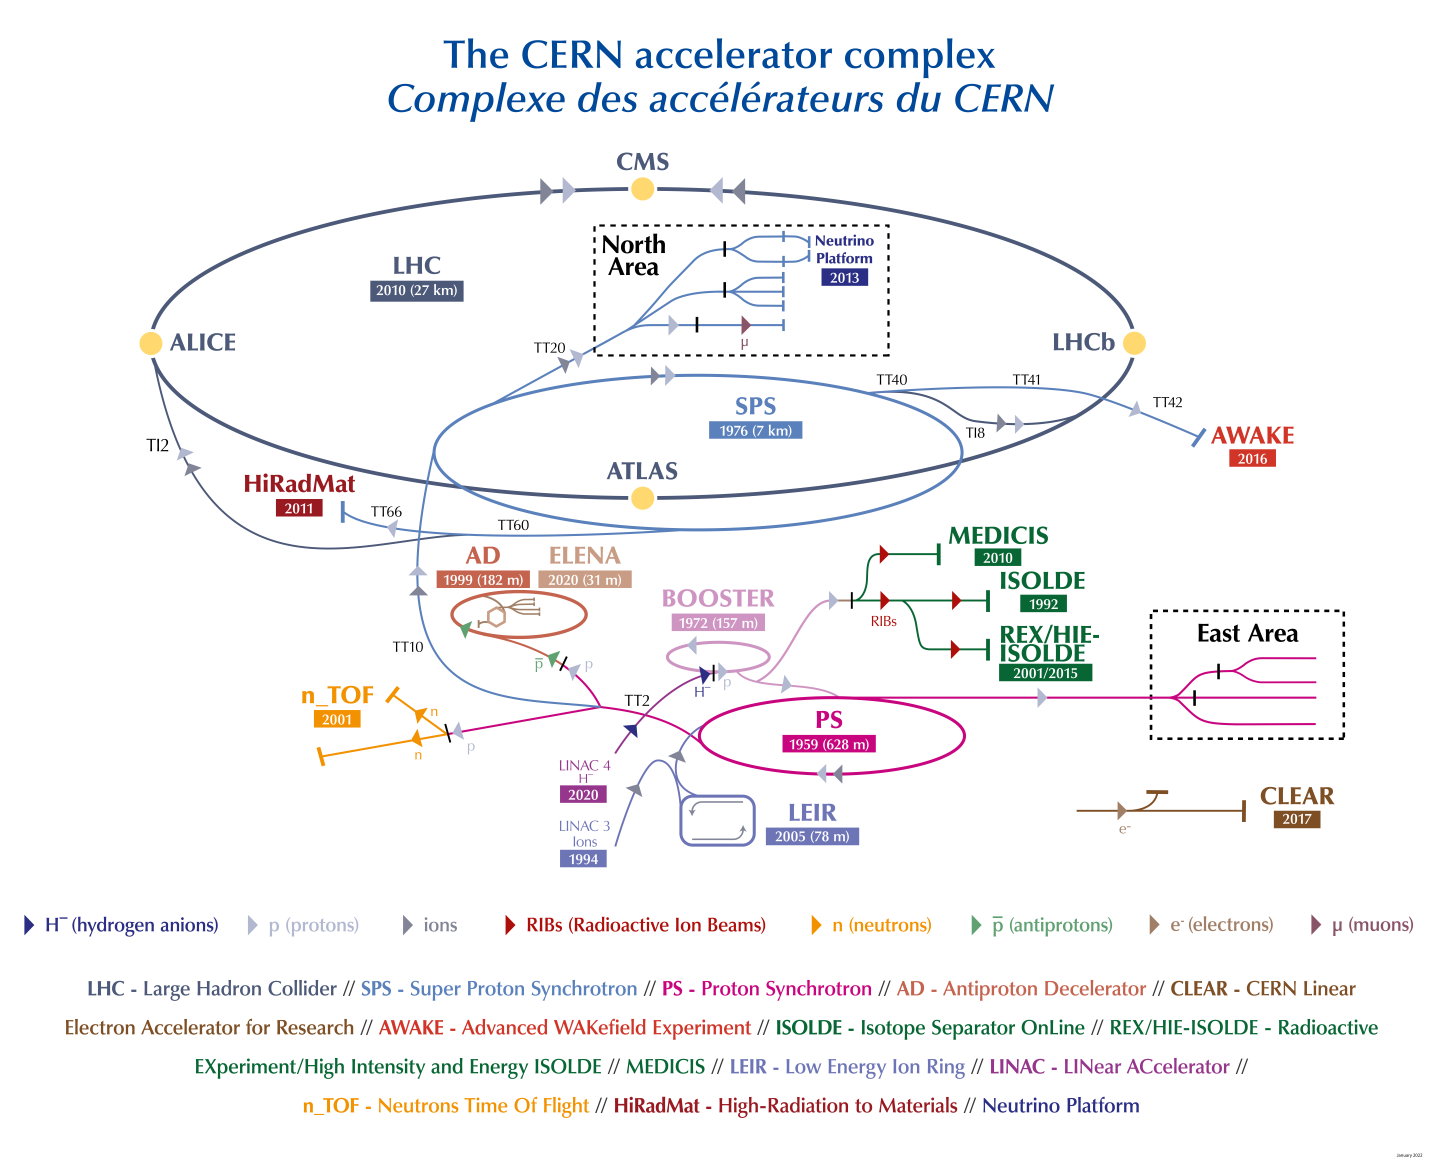
\includegraphics[width=1\textwidth]{images/cern_complex.png}
    \caption{Schematic illustration of the accelerator complex at CERN. Most accelerators are both
    used as injectors for the LHC or to provide beams to fixed target
    experiments~\cite{noauthor_cern_2022}.}
    \label{fig:introduction:cern_complex}
\end{figure}


% --------------------------------
%              LHC
% --------------------------------
\subsection{\review{The Large Hadron Collider}}

The Large Hadron Collider (LHC), is a circular particle accelerator primarily designed to collide
protons for fundamental particle physics research. It can, occasionally over the year, also collide
ions such as oxygen or lead for specifics studies. At the time of writing, in 2024, it holds several
records, such as being the largest and most powerful accelerator in the world, being near 27km long.
The LHC is composed of two beams pipes, being able to accelerate two particle beams from an
injection energy of $450$GeV to an energy of $6,800$GeV, before colliding them in four detectors:
ATLAS, CMS, Alice and LCHb.

Well publicized, the LHC is often depicted via its superconducting dipole magnets, housed in a blue
cryostat, aimed at cooling the coils. \cref{fig:3d_cut_dipole} shows a 3D cut of such magnets. The
LHC is in majority composed of those \textit{main} dipoles, as it holds $1,232$ of them, being each
about 14 meters long. Superconducting materials like Niobium-Titanium (NbTi) are utilized, as
conventional materials such as copper would melt under the current strain. There are indeed around
$12,000$ amperes supplied to generate the magnetic fields necessary for bending the trajectory of
the particles.
Those particles travel at nearly the speed of light (more precisely, $99.99999905\%$ of it),
effectively going around the tunnel about $11,200$ times per second.

\begin{figure}[!htb]
    \centering
    \includegraphics[width=0.8\textwidth]{chapters/01_Introduction/images/lhc_3D_cut.png}
    \caption{3D cut of a main LHC dipole~\cite{noauthor_cern_nodate}. Both beam pipes can be seen
    surrounded by the coils, strongly clamped by the yokes.}
    \label{fig:3d_cut_dipole}
\end{figure}


% -------------------------------
%   Straight Sections and Arcs
\subsubsection{Straight Sections and Arcs}

The LHC is not a perfect circle. It is indeed composed of four \textit{straight} sections, called
the \textit{Interaction Regions} (IPs) where detectors or specific instrumentation are placed. Connecting
those sections, the \textit{arcs} are where the majority of the magnets and their correctors are
located along with some instrument like beam position monitors.
\cref{fig:introduction:lhc_irs} shows the arcs as well as the purpose of each straight section,
housing either specific instrumentation or detectors.

\begin{figure}[!htb]
    \centering
    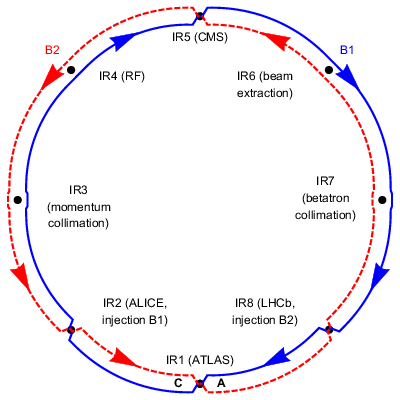
\includegraphics[width=0.5\textwidth]{./images/irs.png}
    \caption{Schematic of the LHC layout.}
    \label{fig:introduction:lhc_irs}
\end{figure}


% -------------------------------
%          Arc Cells
\subsubsection{Arc Cells}

Each arc is made up of 23 cells. Magnets are organized in a standard FoDo structure
(see \ref{section:courant_snyder}), as shows \cref{fig:introduction:lhc_arc_cell}.
\textit{Dipoles} are responsible for bending the trajectory of the particles. Their associated
correctors, the orbit correctors, mitigate any possible drift in path.
\textit{Quadrupoles} are used to control the beam size along the ring. Their effect is focusing in
one plane and defocusing in the other. Their associated correctors control the oscillations of the
beam (see tune, \ref{section:courant_snyder}) and possible field imperfections.
\textit{Sextupoles} correct chromaticity, being a misfocus from quadrupoles due to particles having
a different momentum than the reference particle.
\textit{Octupoles} are used to stabilize the beam by introducing Landau
Damping~\cite{gareyte_landau_1997}. The associated correctors correct higher order chromaticity
effects as well as amplitude dependant tune shifts.
\textit{Decapoles} correctors aim at correcting a even higher chromaticity order.

\begin{figure}[H]
    \centering
    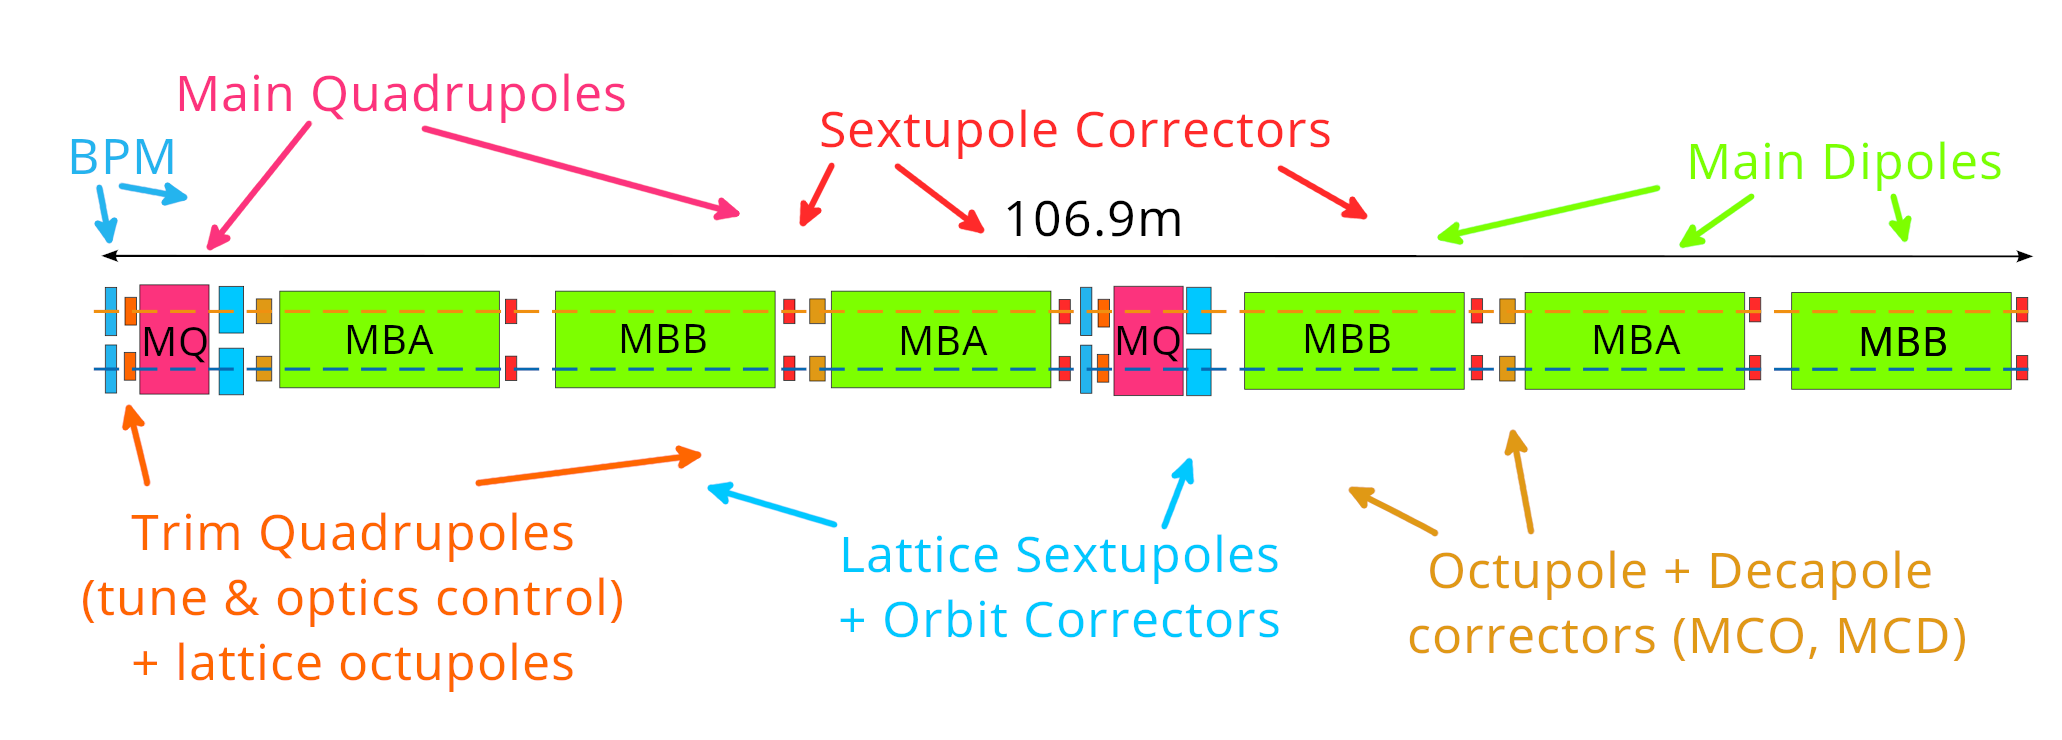
\includegraphics[width=1\textwidth]{./images/lhc_cell.png}
    \caption{Schematic of an LHC Arc cell~\cite{bruning_lhc_2004}.}
    \label{fig:introduction:lhc_arc_cell}
\end{figure}



% -------------------------------
%            Cycles
\subsubsection{\review{Cycles}}

During the operation of the LHC, the machine goes through several states. Those states of the
machine~\cite{wenniger_lhc_2019} have been defined for specific scenarios.

A common example is the operational cycle of the LHC, shown in \cref{fig:cern_complex:cycle}. The
magnets are first pre-cycled~\cite{bottura_pre-cycles_2010} without any beam circulating, to get
them back to a reproducible state. Their current is then increased to accept particles at the 
injection energy of 450GeV. In order to assess the good working condition of the machine, a probe
bunch of reduced intensity is first injected. The number of bunches and their intensity is then
ramped up to attain the desired scheme needed for collisions. This scheme varies throughout the year
depending on the demands of the experiments. The number of bunches and intensity can also be lowered
to keep the machine safe. A common scheme in 2024 is to inject about 2350 bunches with around
$10^{11}$ particles each for collisions.
Optics measurements, due to their destructive nature, typically use between one and three
\textit{pilot} bunches at a lower intensity of $10^{10}$.

The magnets current is them ramped along with the voltage injected in the RF system, to accelerate
particles to an energy of 6.8TeV. While doing so, the beam is squeezed in a first pass at the
Interaction Points. A second pass is done after the ramp is over, to reach a $\beta* = 30cm$ at the
ATLAS and CMS experiments to achieve a small beam size. Crossing-angles are then introduced to make
the beams colliding.

\begin{figure}[!htb]
    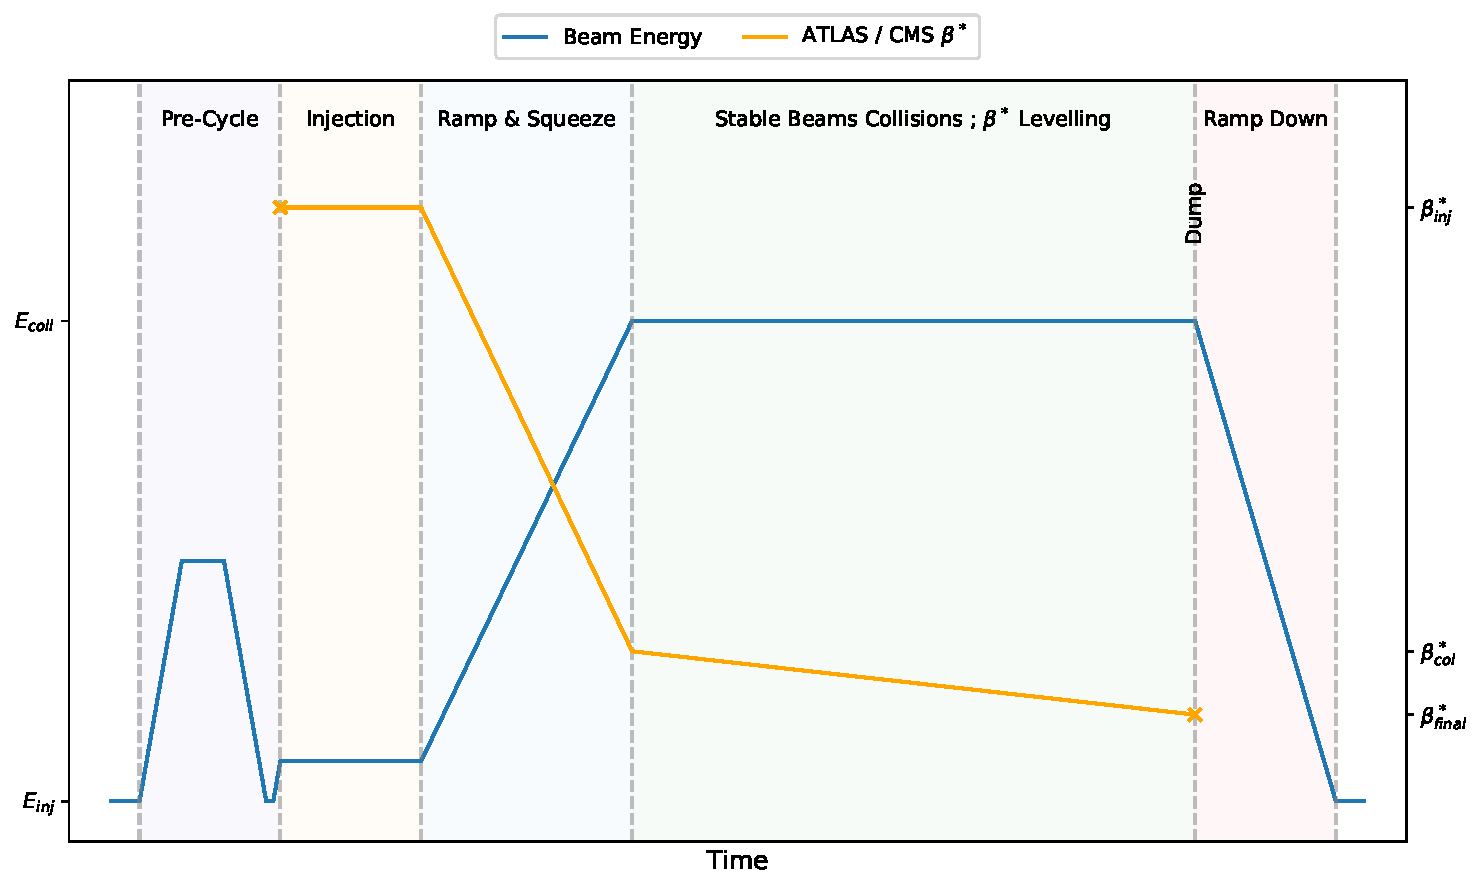
\includegraphics[width=\textwidth]{./images/lhc_cycle.pdf}
    \caption{Simplified illustration of a standard LHC cycle. Courtesy of Félix
    Soubelet~\cite{felix_soubelet_local_2023}.}
    \label{fig:cern_complex:cycle}
\end{figure}


% -------------------------------
%   Harmonics and Field Errors
\subsubsection{\review{Magnetic Fields}}

The magnetic fields of the LHC are created via the coils of the magnets. Real-life magnets never
have a single field as one would like. Instead, so called \textit{allowed harmonics} exist due to
the geometry of the coil. As such, the main dipoles of the LHC can exhibit fields similar to
sextupoles, decapoles, decatetrapoles and so on~\cite{deniau_magnetic_2009}. Manufacturing
imperfections also add fields errors outside of the scope of the allowed ones. Dipoles are indeed
found to generate octupolar field errors.

During the design of the LHC, the main dipoles have been identified to generate significant field
errors. Magnetic measurements of those various fields were thus taken and magnetic tables built
based on real-life magnets nowadays installed in the machine. Those magnetic tables, computed for
each LHC configuration by \textit{WISE}~\cite{p_hagen_wise_2006} are used by simulation softwares.
Predictions of field errors and compensating strength for the correctors is computed by the Field
Description for the LHC (\textit{FiDeL}, \cite{noauthor_fidel_2021}). FiDeL is used in the LHC
control system in operation to steer the beams.

%\begin{figure}[H]
    %\centering
    %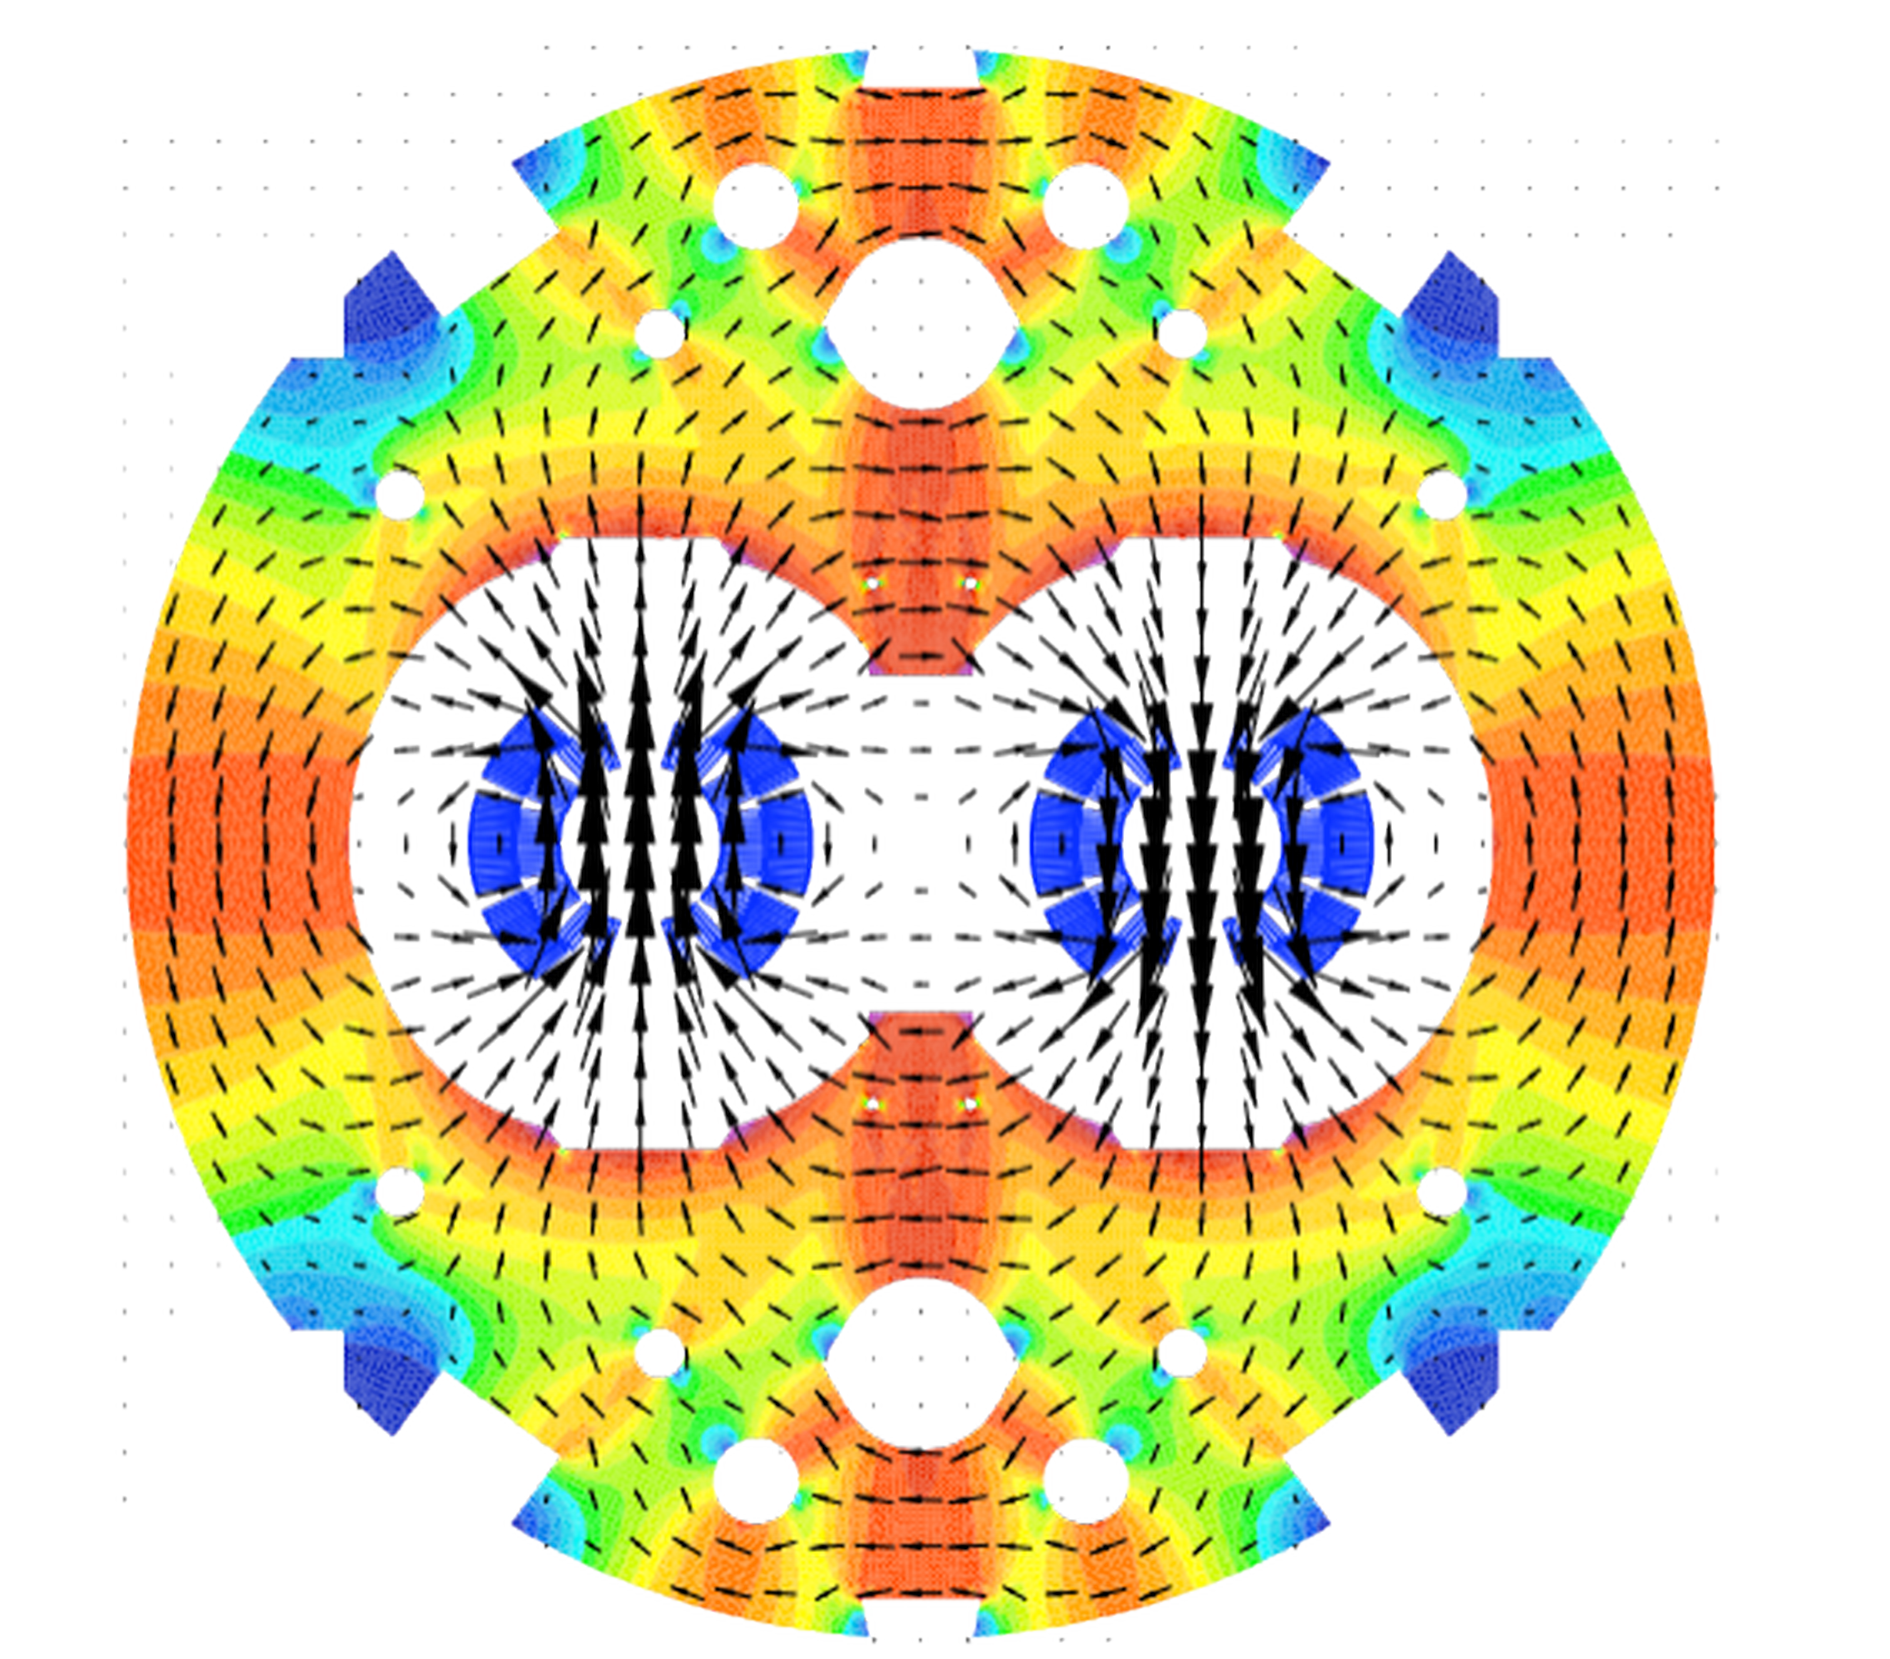
\includegraphics[width=0.5\textwidth]{./images/main_dipole_fields.png}
    %\caption{Magnetic field in a dipole magnet~\cite{deniau_magnetic_2009}.}
    %\label{fig:decapoles:magnetic_field_dipole}
%\end{figure}


% == Software
\section{\review{Tools and Softwares}}

In order to perform the measurements, analysis and simulations presented in this thesis, various
tools and softwares have been developed, used and contributed to.

Optics simulations have been done mainly in MAD-X~\cite{deniau_mad-x_nodate} and PTC.
MAD-NG~\cite{deniau_mad-ng_2020} and
Xsuite~\cite{g_iadarola_xsuite_nodate} have also been explored for specific tasks such as free RDT
simulations and GPU tracking.

Analysis of chromaticity measurements are done via a newly developed graphical
interface~\cite{m_le_garrec_non-linear_2022} written in Python. This tool makes cleaning of the raw
signal data, its analysis and results export more reliable and easier.

Overall, analysis of turn-by-turn measurements is supported by a large panel of libraries written by
the OMC team in Python and Java. Contributions have mainly been made to extended the following
packages:


\begin{itemize}
    \item \textbf{Beta-Beat GUI}~\cite{omc-team_beta-beat_2008}, Graphical interface for turn-by-turn measurements visualization and
    analysis.
    \item \textbf{OMC3}~\cite{omc-team_omc3_2021}, Main optics analysis and corrections software.
    \item \textbf{Beta-Beat.src}~\cite{omc-team_beta-beatsrc_2018}, Old analysis software, now
    replaced by OMC3.
    \item \textbf{pylhc.github.io}~\cite{omc-team_omc_2020}, Website of the OMC team with package
    documentation, examples and useful resources.
\end{itemize}

% === Concepts of Accelerator Physics
\chapter{Concepts of Accelerator Physics}
\thumbforchapter{}
\chaptertoc{}


\begin{enumerate}
    \color{red}
    \item Fields
    \begin{enumerate}
        \item Multipole Expansion
        \item Field normalization
        \item European convention
    \end{enumerate}
    \item Hamiltonian
    \item Coordinates
    \begin{enumerate}
        \item Courant Snyder, twiss parameters an phase space
        \item Linear Maps
        \item Non-Linear maps
        \item Normal Form \& RDT \& resonance diagram
    \end{enumerate}
    \item Linear optics: dispersion, coupling, momentum compaction
    \item Chromaticity

    \begin{enumerate}
        \item Combined effect of multipoles
        \item Amplitude Detuning
        \item Chromtic Amplitude Detuning
        \item Dynamic Aperture
    \end{enumerate}
    \item Luminosity
\end{enumerate}
\chapter{Optics Measurements and Corrections}
\thumbforchapter{}
\chaptertoc{}


\section{\review{Beam Instrumentation}}


% ============================================
%          Beam Position Monitors
% ============================================
\subsection{\review{Beam Position Monitors}}

Beam Position Monitors (BPMs) are one of the most utilized and essential elements of beam 
diagnostics in particle accelerators. In the LHC, most of the BPMs are dual plane, and thus composed
of four electrodes, distributed as two per plane. The BPM system consists of over than 550 BPMs pear
beam, positioned along the ring, in the arcs and the IPs. The most common type, the
\textit{curved-button}, shown in \cref{fig:beam_instrumentation_bpm_button}, is typically placed
near quadrupoles~\cite{wendt_bpm_2020}.

\begin{figure}[!htb]
    \centering
    \begin{subfigure}[b]{0.45\textwidth}
        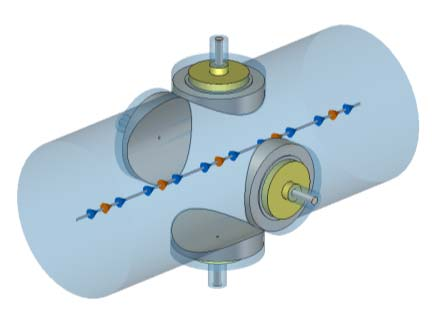
\includegraphics[width=\textwidth]{images/lhc_bpm_button.jpg}
        \caption{Button \textit{"BPM"} type BPM of the LHC~\cite{wendt_bpm_2020}.}
        \label{fig:beam_instrumentation_bpm_button}
    \end{subfigure}
    \hfill
    \begin{subfigure}[b]{0.45\textwidth}
        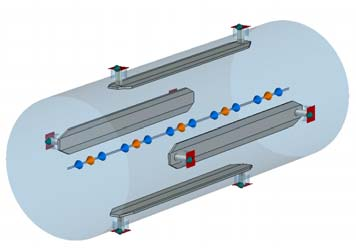
\includegraphics[width=\textwidth]{images/lhc_bpm_stripline.jpg}
        \caption{Stripline \textit{"BPMSW"} type BPM of the LHC~\cite{wendt_bpm_2020}.}
        \label{fig:beam_instrumentation_bpm_stripline}
    \end{subfigure}
\end{figure}

Other pickups such as the \textit{stripline}, shown in
\cref{fig:beam_instrumentation_bpm_stripline}, albeit more complex and expensive, offer a better
signal to noise ratio and are capable of identifying the direction of the
beam~\cite{wendt_bpm_2020}. Such features are essential for the LHC, were both beams travel through
the same aperture at the IPs.\\ 
%The BPM response is not linear with the beam position, which requires a post-processing not
%systematically implemented in accelerators beam diagnostics systems. LHC's BPMs have been simulated
%and polynomials fitted to minimize this response error~\cite{a_nosych_geometrical_2014}.


 
% ============================================
%                Collimators
% ============================================
\FloatBarrier
\subsection{\review{Collimators}}

Collimators are a crucial part of the LHC. Their purpose is to protect the machine against beam
losses and clean the outer parts of the beam~\cite{redaelli_lhc_2011}. The energy of the beams in
the LHC is high enough to not only quench the magnets, but to also damage the elements. At
injection energy, with a low intensity pilot bunch, the consequences of a loss are less severe.

%During Run 3, in 2022, a new collimator sequence was introduced, making a safe exploitation
%of the machine possible with more retracted collimators. This made measurements with higher kick
%amplitudes and larger orbit offsets, and thus momentum offsets, possible.


% ============================================
%             Beam Loss Monitors
% ============================================
\subsection{\review{Beam Loss Monitors}}

Beam Loss Monitors are detectors mounted on various elements of the accelerator, such as magnets or
collimators, to detect abnormal losses of particles. They play a crucial role in the protection of
the machine, triggering a dump when losses exceed the threshold set for their respective element. 
BLMs use ionization chambers, working on the same principle as simple Geiger counters: a tube filled
with gas, in presence of a high voltage~\cite{schmidt_machine_2014}. A picture of BLMs mounted on
the LHC is given in \cref{fig:beam_instrumentation:blm1}.

Dashboards in the control room are regularly used to monitor the losses along the ring when
performing optics measurements, as those prove to often be destructive. An example of such a
dashboard is given in \cref{fig:beam_instrumentation:blm2}.

\begin{figure}[H]
    \centering
    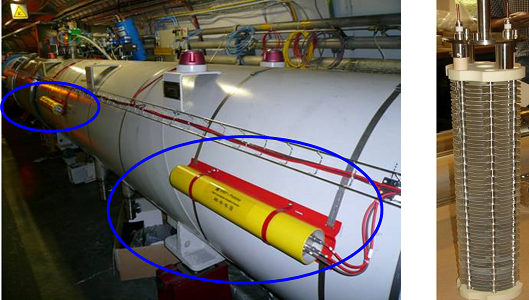
\includegraphics[width=0.6\textwidth]{images/blm.png}
    \caption{Beam Loss Monitors (BLM), in yellow, on the LHC~\cite{schmidt_machine_2014}.}
    \label{fig:beam_instrumentation:blm1}
\end{figure}

\begin{figure}[H]
    \centering
    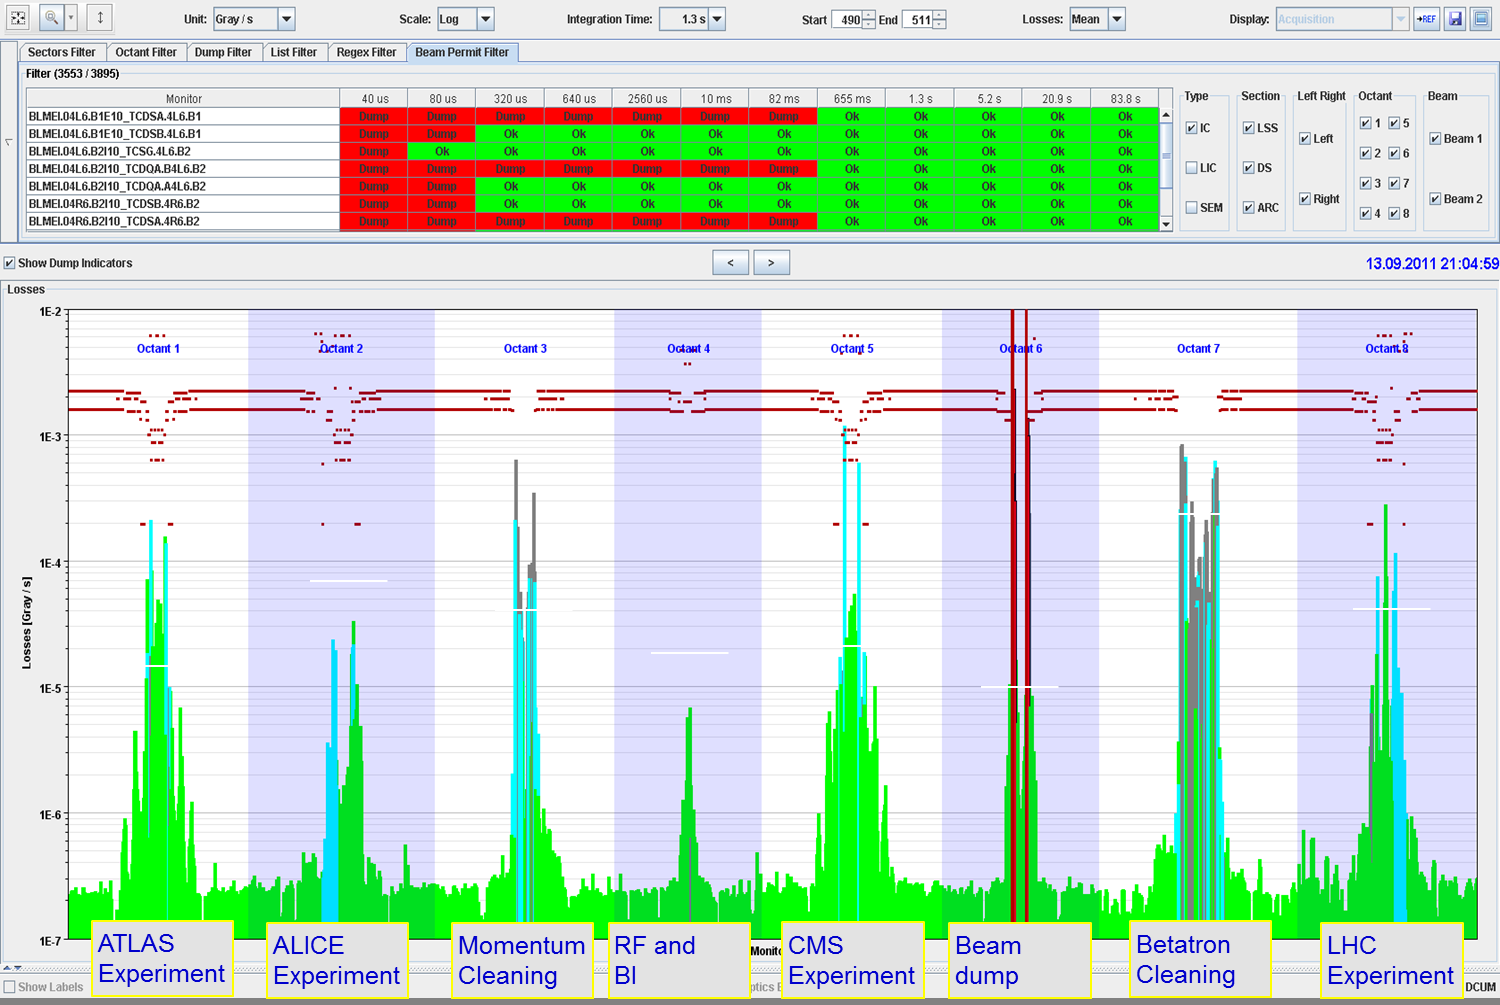
\includegraphics[width=0.6\textwidth]{images/blm2.png}
    \caption{Graphical interface used in the CERN Control Cernter (CCC) for instantaneous losses in
    the LHC~\cite{schmidt_machine_2014}. Different parts of the accelerator have varying dump
    thresholds.}
    \label{fig:beam_instrumentation:blm2}
\end{figure}


% ============================================
%                   BCT
% ============================================
\subsection{\review{Beam Current Transformer}}

The Beam Current Transformer (BCT) is a device used to measure the intensity of a particle beam by
detecting the current induced by the moving charge of the beam as it passes through the coil of the
BCT. The beam effectively acts as a primary coil and induces a current in the secondary coil of the
transformer.
The BCTs are designed to be able to measure intensities from pilots bunches of 8µA to total beams of
more than 860mA~\cite{odier_dcct_2009}. During optics measurements, beam intensity is often closely
monitored to ensure data quality, as certain observables may not be detectable at low intensities.

% ============================================
%                   BBQ
% ============================================
\subsection{\review{BBQ System}}

The Base-Band Tune (BBQ) system in the LHC is designed to measure the beam's tune via its
turn-by-turn signal. It operates by detecting and analyzing the signals of diode
peak-detectors~\cite{boccardi_first_2009,gasior_high_2005}. The system further implements processing
hardware and software, transmitting the acquired data to the control and logging systems.  The
system can operate with no explicit excitation, relying on the residual beam oscillations, or by
using tune kickers or frequency sweeps~\cite{boccardi_first_2009}.


% ============================================
%                 AC-Dipole
% ============================================
\subsection{\review{AC-Dipole}}

The AC dipole of the LHC is a crucial component for optics studies. Its primary function is to
excite the beam into large coherent oscillation, achieved by applying a sinusoidally oscillating
dipole field~\cite{miyamoto_parametrization_2008}. By ramping up and down adiabatically the
amplitude, large coherent oscillations can be produced without any decoherence or emittance growth.
\Cref{fig:ac_dipole} shows an example of a simulation made with an AC-Dipole. Exciting the beam to
large amplitudes make the study of linear optics, such as beta-beating easier, and that of non
linear optics such as resonances possible.

\begin{figure}
    \center
    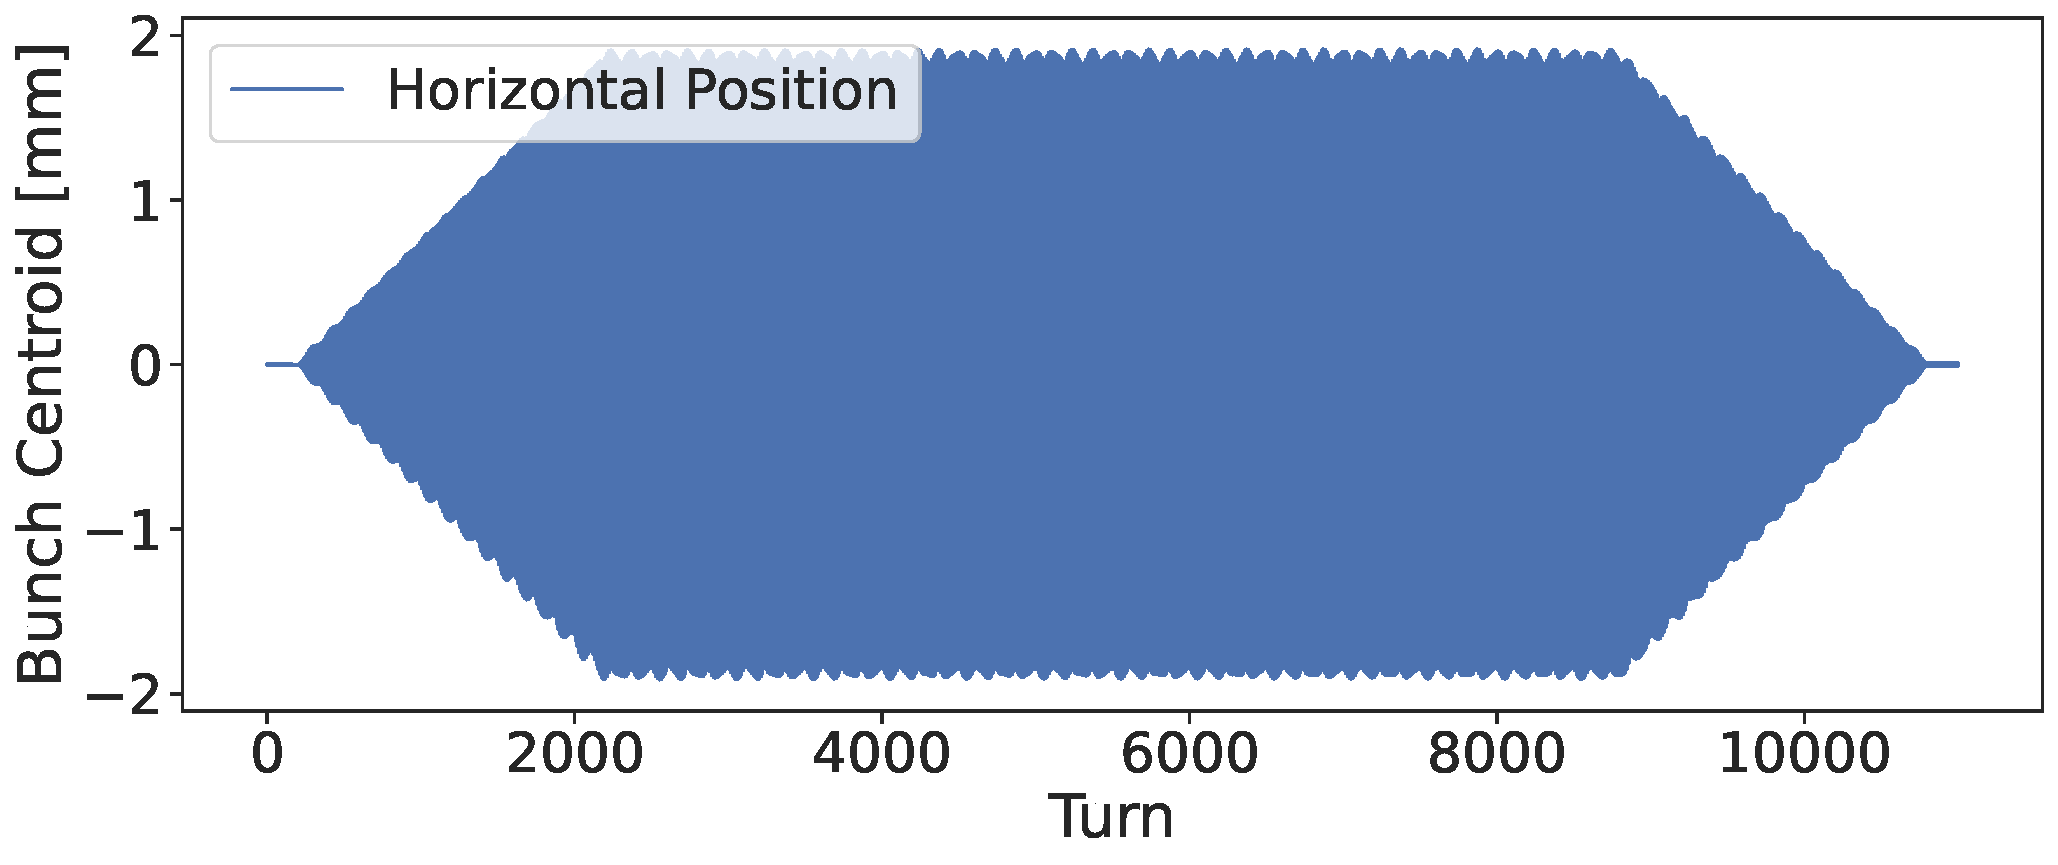
\includegraphics[width=0.85\textwidth]{./images/ac_dipole_tbt.pdf}
    \caption{Simulated turn by turn data with an AC-Dipole first ramping up then down.} 
    \label{fig:ac_dipole}
\end{figure}

The AC-Dipole is set to oscillate at a frequency $Q_d$, different from the natural tune of the
machine $Q$ and thus introduces systematic effects that needs to be compensated during the optics
analysis. The transverse position of a particle under the influence of the AC-Dipole, at turn number
$n$ and observation point $s$, is given
by~\cite{serrano_lhc_2010,tomas_normal_2002,white_direct_2013}:

\begin{equation}
z(s, n) = \frac{BL}{4\pi\rho\delta_z} \cdot \sqrt{\beta_z(s) \beta_{z,0}} \cdot \cos \left( 2 \pi Q_{d,z}n + \phi_z(s) + \phi_{z,0}\right),
\label{eq:ac_dipole}
\end{equation}

where $B$ is the amplitude of the oscillating magnetic field, $L$ the length of the AC-Dipole,
$B\rho$ the magnetic rigidity, $\delta$ the difference between $Q_d$ and $Q$, $\beta$ and $\beta_0$
the beta function at the observed point and the AC-Dipole, $\phi$ and $\phi_0$ the phase advance at
the observed point and of the AC-Dipole.
% ===============================
%        Optics Measurements
% ===============================

\subsection{Turn by Turn}





% ================================================= 
%                   Chromaticity
\subsection{Chromaticity}

% --- Procedure ---
\subsubsection{Procedure}

Chromaticity measurements are typically performed by varying the RF frequency to induce a change of momentum offset $\delta$, while measuring the tune.
The momentum offset $\delta$ being related to the RF frequency and the momentum compaction factor $\alpha_c$:

\begin{equation}
    \delta = - \frac{1}{\alpha_c} \cdot \frac{\Delta f_{RF}}{f_{RF,nominal}}
    \label{eq:dpp_rf}
\end{equation}

Frequency steps of 20Hz every 30 secondes are typically taken to compromise between number of data points, precision of the tune estimate, and duration of the measurement.
Once beam losses, registered by the Beam Loss Monitors (BLM), are deemed too high, the frequency is reverted back to its nominal value in larger steps. The same procedure is then re-applied in the negative. Figure \ref{fig:measurements:rf_scan} shows a typical RF scan performed to measure chromaticity in the LHC.

\begin{figure}[H]
    \centering
    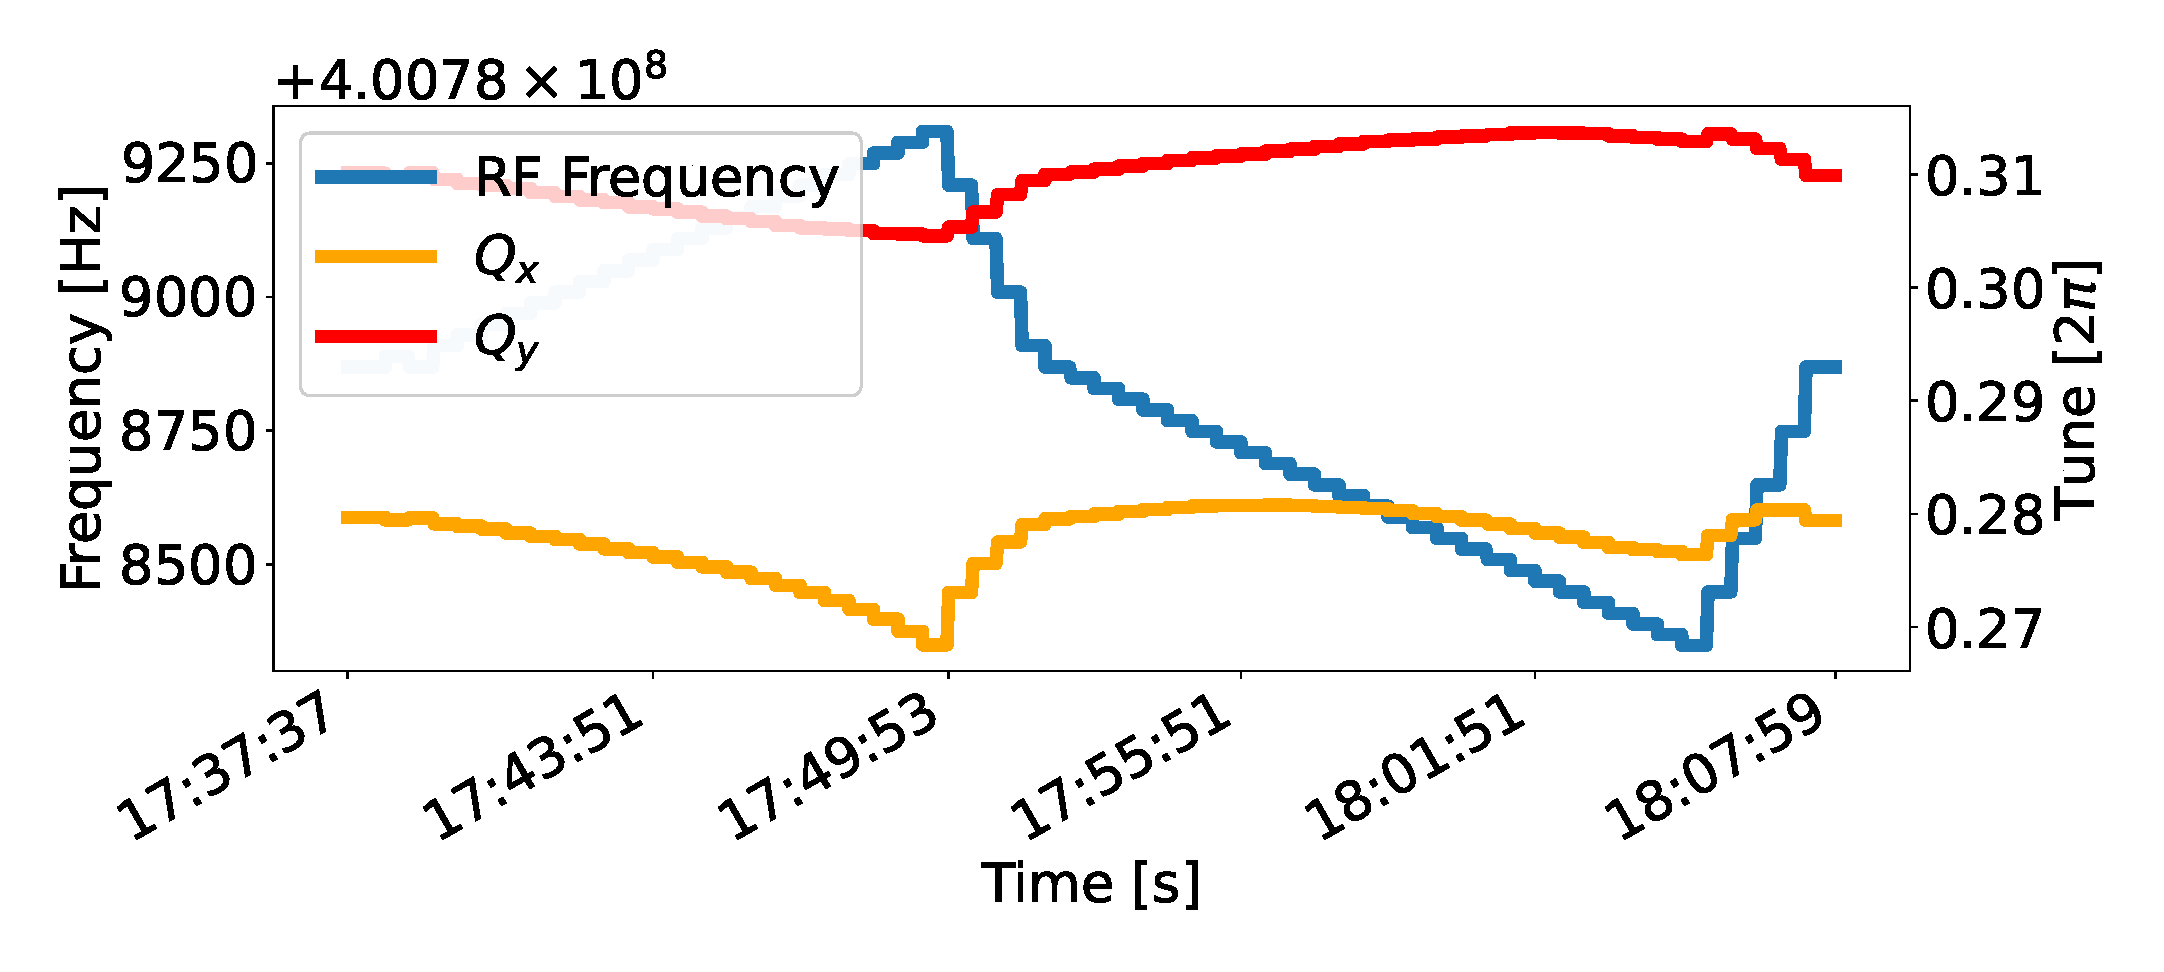
\includegraphics[width=1\textwidth]{images/rf_scan.pdf}
    \caption{Observation of the tune dependence on momentum offset, created by a shift of RF frequency}
    \label{fig:measurements:rf_scan}
\end{figure}




% --- Analysis and Fit ---
\subsubsection{Analysis}

\section{Correction Principles}


% ===============================
%        Response Matrix
% ===============================
\subsection{\review{Response Matrix}}

A response matrix is a linear equation system that describes the change of an observable for a set of individual multipole strengths. By taking the pseudo-inverse of this matrix and multiplying it to the measured observables, a set of corrector strengths if obtained that can replicate the measured value. Taking the opposite sign then gives a correction.
This technique is routinely used to correct, amongst others, \beta-beating as well as Resonance Driving Terms. In situations where measurements are taken at each BPM for a particular observable, the corresponding response matrix ends up containing over 500 values per corrector, for a single beam.

Individual MAD-X simulations are run with a single multipole powered at a time. The resulting parameter values (e.g. \beta-beating) are then compared to those obtained from a simulation without any powering, allowing to determine the specific impact of each multipole.

A response matrix is thus created following eq.\ref{eq:resp_matrix}, for a matrix of observables $O$, a reference matrix of observables without any corrector $O_R$ and a fixed multipole strength $k$. Given measured data $M$, the set of correctors needed to compensate the values can be obtained by taking the pseudo-inverse of the matrix in eq.\ref{eq:resp_matrix_inverted}.

\begin{equation}
  R = \left(O - O_R \right) \cdot \frac{1}{k}
  \label{eq:resp_matrix}
\end{equation}

\begin{equation}
  \begin{bmatrix}
    k_1 \\
    \vdots \\
    k_n \\
  \end{bmatrix}
  = -(R^{+} \cdot M)
  \label{eq:resp_matrix_inverted}
\end{equation}
 
Response matrices are very versatile and can combine several observables to be corrected by the same multipoles. One example, detailed later in this thesis, is the third order chromaticity and the resonance driving term $f_{1004}$, both contributed to by decapoles.

\subsubsection{Example}

In this example, simulations are run with MAD-X PTC to correct the third chromaticity in the LHC.
$Q'''$ is taken from \verb|ptc_normal| for each beam and axis, with \verb|MCDs|, decapole correctors, powered with a fixed strength one at a time. A scaling factor is applied to get the change of chromaticity for one unit of $K_5$.
8 correctors are used, which strengths are denoted $k_1$ through $k_8$.
Transposes are only used to make the equations easier to display.\\
The values in Tab.\ref{table:resp_matrix_example} are corrected via 
Eq.~\eqref{eq:resp_matrix_inverse_example} after having built the response matrix in Eq.~\eqref{eq:resp_matrix_example}.

\begin{table}[H]
  \center
  \begin{tabular}{c c c}
      Observable & Value \\
      \hline
      $Q'''_x$ & -666111 \\
      $Q'''_y$ &  121557 \\
  \end{tabular}
  \caption{Example chromaticity values to correct via a response matrix}
  \label{table:resp_matrix_example}
\end{table}

% ====
\vspace{0.4cm}
\begin{equation}
  R
  %
  =
  %
  \left(
    %{\text{Individual} \atop \text{simulations}}
    {\genfrac{}{}{0pt}{0}{\text{Individual}}{\text{simulations}}}
    \left\{
      \begin{bNiceMatrix}
       -155899  &  122004 \\  
       -254584  &  138368 \\
       -122715  &  106709 \\
       -218597  &  110686 \\
       -134140  &  106463 \\
       -245791  &  118951 \\
       -147035  &  116544 \\
       -219537  &  112317 \\
        \CodeAfter
        \OverBrace{1-1}{1-1}{Q'''_x}[yshift=2mm]
        \OverBrace{1-2}{1-2}{Q'''_y}[yshift=2mm]
      \end{bNiceMatrix}^T
    \right.
    -
    \left.
    \begin{bNiceMatrix}
       5135 \\
       8470 \\
      \CodeAfter
      \OverBrace{1-1}{1-1}{\scriptstyle \text{Reference}}[yshift=2mm]
    \end{bNiceMatrix}
    \right\}
    {\genfrac{}{}{0pt}{0}{Q'''_x}{Q'''_y}}
  \right)
  %
  \cdot
  %
  \underbrace{\frac{1}{-1000}}_{\text{Corrector strength}}
  \label{eq:resp_matrix_example}
\end{equation}
\vspace{0.5cm}


% Inverting the response matrix
\begin{equation}
    \begin{matrix}
      k_1 \\
      k_2 \\
      k_3 \\
      k_4 \\
      k_5 \\
      k_6 \\
      k_7 \\
      k_8 \\
    \end{matrix}
  \left\{
  \begin{pmatrix}
     -1235 \\
      1032   \\  
     -1394  \\ 
      1449   \\ 
     -1043  \\ 
      1864   \\ 
     -1187  \\ 
      1369   \\ 
  \end{pmatrix}
  \right.
  %
  =
  %
  -R^{+} 
  %
  \cdot
  %
  \left.
  \begin{pNiceMatrix}
      -666111 \\
      121557 \\
  \end{pNiceMatrix}
  \right\}
  %{\text{Measured} \atop \text{values}}
  {\genfrac{}{}{0pt}{0}{\text{Measured}}{\text{values}}}
  \label{eq:resp_matrix_inverse_example}
\end{equation}





% ===============================
%    Chromaticity Global Trim
% ===============================
\subsection{\review{Global Trims for Chromaticity}}

% ~~~~~~~~~~~~~~~~~~~~~~~~~~~~~
% The script for the linearity can be found in
% /afs/cern.ch/work/m/mlegarr2/public/jupyter/chromaticity/simulations/linearity_dq3_mcd

As per the placement of the MCO and MCD spool piece correctors in the LHC 
layout~\cite{maclean_commissioning_2016-1}, $\beta$-functions at their location are slightly
different from arc to arc. This slight imbalance leads theoretically to the possibility of
correcting the horizontal and vertical axes of the second and third order chromaticity
independently, via a response matrix approach. In practice, the required strength to do so would
exceed those of the design of the correctors.

Another way to correct the chromaticity is via a global uniform trim, where every available
corrector is powered to the same strength.  Simulations are run with \verb|ptc_normal| via MADX-PTC
to obtain the response in chromaticity for a given strength. Chromaticity being linear with
multipole strength, an affine function can be determined for each axis. Figure
\ref{fig:corrections-dq3_versus_k5} shows a simulation with several MCD strengths, highlighting this
linear relation between $Q'''$ and $K_5$, while
Equation~\eqref{eq:corrections:chromaticity_affine_function_ptc} shows an example of such functions computed
at injection energy for the 2022 optics.

\begin{figure}[H]
  \centering
  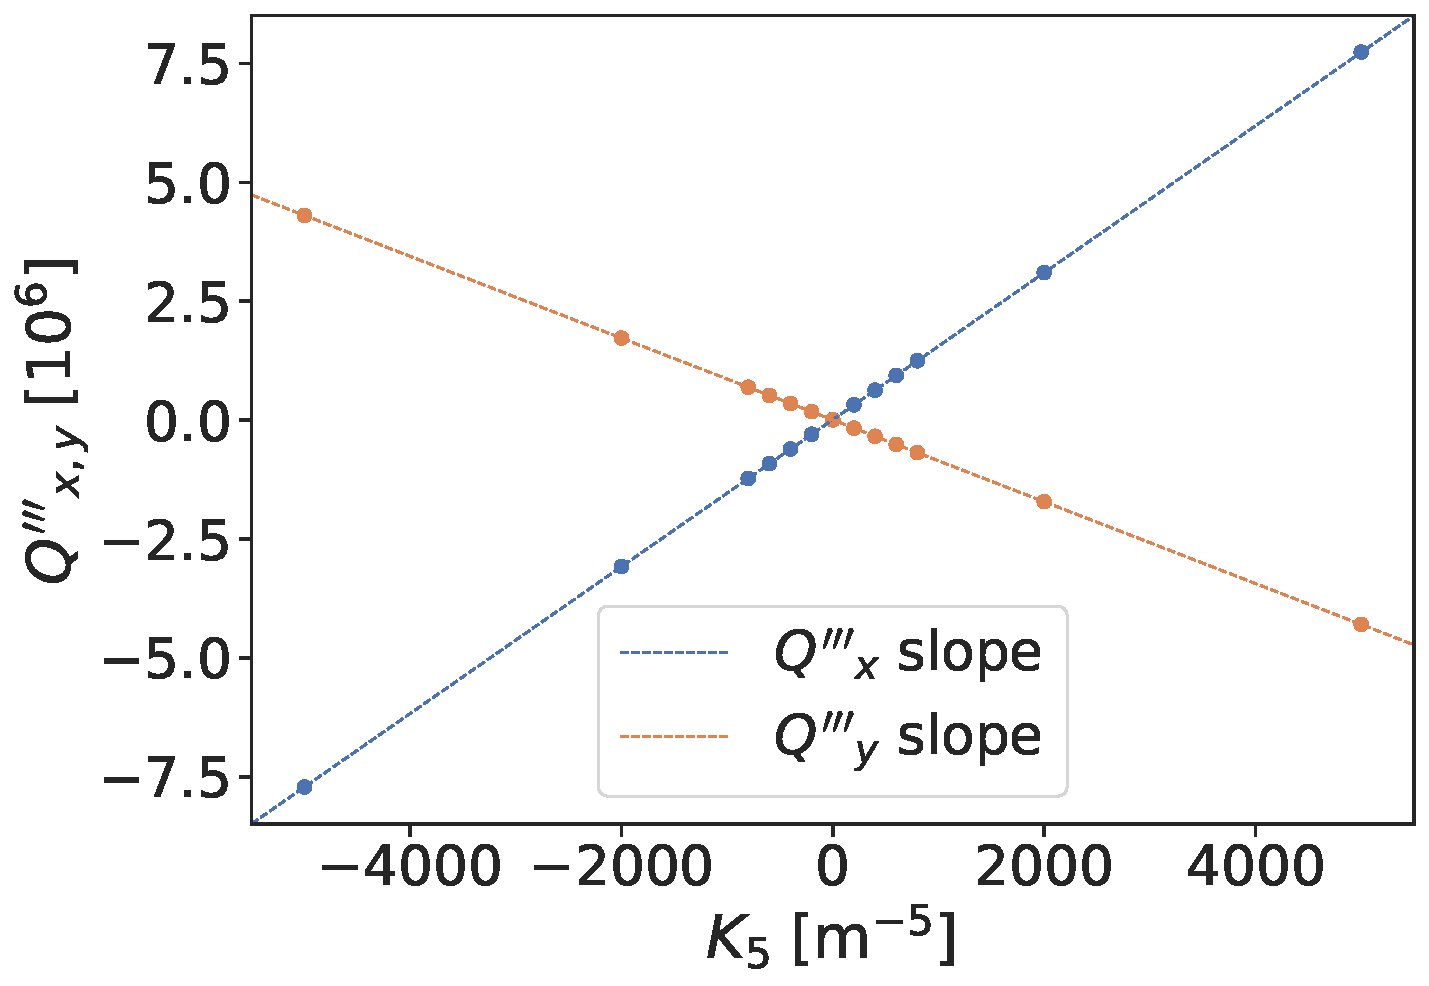
\includegraphics[width=0.6\textwidth]{images/dq3_k5.pdf}
  \caption{Linear relation between the third order chromaticity and decapole corrector strengths,
           simulated with MADX-PTC.}
  \label{fig:corrections-dq3_versus_k5}
\end{figure}

\begin{equation}
  \begin{aligned}
    &Q'''_x = 1533 \cdot \Delta K_5 + 6680 \\
    &Q'''_y = -860 \cdot \Delta K_5 + 5647
  \end{aligned}
  \label{eq:corrections:chromaticity_affine_function_ptc}
\end{equation}

Only the linear part is relevant, as the offset is generated by other multipoles and field errors.
It is thus constant for a configuration where only the relevant spool pieces are used.

Corrections involve minimizing both axes, typically where $Q'''_x$ meets $Q'''_y$:

\begin{equation}
  \Delta K_5 = -\frac{(Q'''_x - Q'''_y)}{\text{slope}_{Q'''_x} - \text{slope}_{Q'''_y}}
  \label{eq:corrections:chromaticity_global_correction}
\end{equation}
% ====


% ===========================================================================
%                  Theory
% ===========================================================================
\chapter[Theory]{Theory}

\hypertarget{units}{%
\section{Units}\label{units}}

\begin{itemize}
\item
  Joules: \[1 J = 1 N \cdot m = 1 kg \cdot m^2 \cdot s^{-2}\]
\item
  Electronvolt:

  \begin{itemize}
  \tightlist
  \item
    \(eV = e \cdot V\)

    \begin{itemize}
    \tightlist
    \item
      e: elementary charge
    \item
      V: volt
    \end{itemize}
  \item
    \(1 eV = 1.602176634 \cdot 10^{-19} J\)
  \end{itemize}
\item
  Momentum:

  \begin{itemize}
  \tightlist
  \item
    \(p\) in \(kg.m.s^{-1}\)
  \item
    \(p\) in \(eV.c^{-1}\): \(J \cdot c^{-1} = kg.m.s^{-1}\)
  \end{itemize}
\item
  Tesla \[T = \frac{V \cdot s}{m}\]
\end{itemize}

\newpage

\hypertarget{definitions}{%
\section{Definitions}\label{definitions}}

\hypertarget{some-math-definitions}{%
\subsection{Some Math Definitions}\label{some-math-definitions}}

\begin{itemize}
\item
  Harmonic Oscillator \[F = -kx\] \[x'' = -\frac{k}{m}x \]
\item
  Magnetic rigidity, used for dipoles: \[B\rho = \frac{p}{q}\]

  \begin{itemize}
  \item
    B: magnetic field {[}\(T\){]}
  \item
    \(\rho\): radius of curvature of the orbit {[}\(m\){]}
  \item
    p: momentum {[}\(eV/c\){]}
  \item
    q: particle charge {[}\(e\){]}
  \item
    Can be expressed as \[B \rho = 3.3356 p\] if \(p\) is in GeV/c
  \end{itemize}
\item
  Magnets orders
\end{itemize}

\begin{center}
  \begin{tabular}{lllllll}
  Magnet Letter          & B & Q & S & O & D & T \\
  Number of Poles        & 2 & 4 & 6 & 8 & 10 & 12 \\
  a (skew) designation   & 1 & 2 & 3 & 4 & 5 & 6 \\
  b (normal) designation & 1 & 2 & 3 & 4 & 5 & 6 \\
  K designation          & 1 & 2 & 3 & 4 & 5 & 6 \\
  MADX-K                 & 0 & 1 & 2 & 3 & 4 & 5 \\
  \end{tabular}
\end{center}

\begin{itemize}
\item
  Magnet Strength:
  \begin{equation}K_{n} = \frac{q}{P} (n-1)!B_n\label{eq:magnet_strength}\end{equation}

  \begin{itemize}
  \item
    The unit is given by:

    \begin{itemize}
    \tightlist
    \item
      k1: dipole: \(m^{-1}\)
    \item
      k2: quadrupole: \(m^{-2}\)
    \item
      k3: sextupole: \(m^{-3}\)
    \item
      k4: octupole: \(m^{-4}\)
    \item
      k5: decapole: \(m^{-5}\)
    \item
      k6: dodecapole: \(m^{-6}\)
    \end{itemize}
  \item
    If interested in the \emph{integrated} strength, multiply by
    \emph{m}
  \end{itemize}
\item
  Dispersion is given via:
  \begin{equation}D = \frac{\Delta x}{\delta}\end{equation}
\item
  The relative momentum offset is defined via the reference momentum and
  the momentum
  \begin{equation}\delta = \frac{\Delta P}{P_0} = \frac{P - P_0}{P_0}\label{eq:dpp}\end{equation}
\item
  Relation between the action and the single particle emittance:
  \href{https://journals.aps.org/prab/pdf/10.1103/PhysRevSTAB.17.081002}{Non
  Linear Observables} (eq. 2):
  \begin{equation}2J_{x,y} = \epsilon_{x,y}\end{equation}
\item
  The tune is defined as the derivative of the Hamiltonian relative to
  the action.
  \begin{equation}Q_{x,y} = \frac{\partial \left< H \right>}{\partial J_{x,y}}\end{equation}
\item
  The tune can also be defined as:
  \begin{equation}Q_{x,y} = \frac{1}{2 \pi} \oint \frac{1}{\beta_{x,y}(s)} \,ds\end{equation}
\item
  The phase advance in the \(x\) plane, between two elements \(w\) and
  \(j\), in the accelerator is given by
  \href{https://arxiv.org/abs/1711.06589}{AnalyticFormulasFranchi}:
\end{itemize}

\begin{equation}
\begin{cases} 
  \Delta \phi_{x,wj} = \left(\phi_{x,j} - \phi_{x,w} \right)              & \mbox{if } \phi_{x,j} > \phi_{x,w}, \\
  \Delta \phi_{x,wj} = \left(\phi_{x,j} - \phi_{x,w} \right) + 2 \pi Q_x  & \mbox{if } \phi_{x,j} < \phi_{x,w}.
\end{cases}
\end{equation}

\newpage

\hypertarget{glossary}{%
\subsection{Glossary}\label{glossary}}

\renewcommand{\glossarysection}[2][]{}
\renewcommand*{\glspostdescription}{\vspace{-8pt}}
\glsnoexpandfields

\hypertarget{equipment}{%
\subsubsection{Equipment}\label{equipment}}

\glsaddall
\vspace{-6\parskip}
\printglossary[type=equipment]

\hypertarget{beam}{%
\subsubsection{Beam}\label{beam}}

\glsaddall
\vspace{-6\parskip}
\printglossary[type=beam]

\newpage

\hypertarget{maths}{%
\section{Maths}\label{maths}}

\hypertarget{taylor-series}{%
\subsection{Taylor Series}\label{taylor-series}}

The Taylor series of a multivariable function at the point
\((a_1, \cdots, a_d)\) is defined as:

\begin{equation}\begin{aligned}
  f(x_1, \cdots, x_d) = &f(a_1, \cdots, a_d) \\
                &+ \frac{1}{1!} \sum_{j=1}^{d} \frac{\partial f(a_1, \cdots, a_d)}{\partial x_j} (x_j - a_j) \\
                &+ \frac{1}{2!}\sum_{j=1}^{d}\sum_{k=1}^{d} \frac{\partial^2 f(a_1, \cdots, a_d)}{\partial x_j\partial x_k} (x_j - a_j) (x_k - a_k) \\
                &+ \frac{1}{3!}\sum_{j=1}^{d}\sum_{k=1}^{d}\sum_{l=1}^{d} \frac{\partial^3 f(a_1, \cdots, a_d)}{\partial x_j\partial x_k\partial x_l} (x_j - a_j) (x_k - a_k) (x_l - a_l)\\
                &+ \cdots
\end{aligned}\label{eq:taylor}\end{equation}

\hypertarget{non-linear-transfer-maps}{%
\subsection{Non-Linear Transfer Maps}\label{non-linear-transfer-maps}}

For linear dynamics, linear transfer maps can be used to describe a
particle's position from the elements in the lattice and the particle's
current position. In the non linear case, such a formalism can't be
used. Instead, the Lie operator is used.

\hypertarget{lie-operator}{%
\subsubsection{Lie Operator}\label{lie-operator}}

Resources found in
\href{https://mlegarre.web.cern.ch/mlegarre/Courses/Meghan_RDTpresentation.pdf}{Meghan
McAteer's talk} and Wolski's book.

The Lie operator is defined as:

\[
\colon f \colon = \sum^n_{i=1} \left(\frac{\partial f}{\partial x_i} \frac{\partial}{\partial p_i} 
                           - \frac{\partial f}{\partial p_i} \frac{\partial}{\partial x_i}
                      \right)
\]

With \emph{i} the index of a dimension. So \(x_1\) would be \(x\) and
\(x_2\), \(y\).

The exponential Lie operator \(e^{:f:}\) acting on a function \(g\):

\begin{equation}e^{:f:}g = g + [f, g] + \frac{1}{2} [f, [f, g]] + \cdots\label{eq:Lie}\end{equation}

This is from the usual power series of an exponential:

\[e^{:f:} = \sum^{\infty}_{m=0} \frac{:f:^m}{m!}\]

Where \([f, g]\) is a poisson bracket, still somehow used for historical
reasons:

\begin{equation}[f, g] = \colon f \colon g
\label{eq:poisson_bracket}\end{equation}

Thus, the particle with coordinates \(\vec{x}\) passing through an
element can be mapped using the Hamiltonian of the element (Wolski, eq.
9.6):

\begin{equation}\vec{x}_f = e^{-\Delta s:H:} \vec{x}_0\label{eq:position_non_linear}\end{equation}

For a \emph{thin} lens, we can directly multiply by the length of the
magnet:

\begin{equation}\vec{x}_f = e^{-L:H:} \vec{x}_0\label{eq:position_non_linear_thin}\end{equation}

By combining \cref{eq:Lie} and \cref{eq:position_non_linear}, we obtain:

\begin{equation}
\begin{aligned}
\left[H, \vec{x}_0\right] =& \frac{\partial H}{\partial x} \frac{\partial \vec{x}_0}{\partial p_x} 
                                    -\frac{\partial H}{\partial p_x} \frac{\partial \vec{x}_0}{\partial x} \\
                           &\frac{\partial H}{\partial y} \frac{\partial \vec{x}_0}{\partial p_y} 
                                    -\frac{\partial H}{\partial p_y} \frac{\partial \vec{x}_0}{\partial y}
\end{aligned}
\label{eq:bracket_hamiltonian}\end{equation}

Thus giving us the complete equation:

\begin{equation}
\begin{aligned}
\vec{x}_f &= e^{:H:}\vec{x}_0 \\
          &= \vec{x}_0 + \left[H, \vec{x}_0\right] \\
          &= \begin{pmatrix} x \\ p_x \\ y \\ p_y\end{pmatrix}_0
             + \begin{pmatrix} -\frac{\partial H}{\partial p_x} \\ 
                               \frac{\partial H}{\partial x} \\
                               -\frac{\partial H}{\partial p_y} \\
                               \frac{\partial H}{\partial y}
               \end{pmatrix} \\
\begin{pmatrix} x \\ 
                p_{x} \\
                y \\
                p_{y} 
\end{pmatrix}_f
          &=  \begin{pmatrix} x_0 - \dfrac{\partial H}{\partial p_x} \\ 
                               p_{x0} +\dfrac{\partial H}{\partial x} \\
                               y_0 - \dfrac{\partial H}{\partial p_y} \\
                               p_{y0} +\dfrac{\partial H}{\partial y}
               \end{pmatrix}
\end{aligned}
\label{eq:non_linear_map}\end{equation}

This non linear transfer map is a general map without coupling.

\hypertarget{multipole-expansion}{%
\subsection{Multipole Expansion}\label{multipole-expansion}}

This is the Hamiltonian for a magnetic element with normal strength
component \emph{K} and skew component \emph{J}:

\begin{equation}H = \Re \left[\sum_{n>1} \left( K_{n} + iJ_{n} \right) \frac{(x+iy)^n}{n!} \right]\label{eq:hamiltonian}\end{equation}

This equation is an expansion of the magnetic field into its multipole
components. If we're only interested in one component, the sum can be
dropped and \(n\) set to the desired multipole.

Remark: When writing terms like \(K_1\) it is assumed it is \(K_1(s)\).
Is is important later for the chromaticity where the average is a
circular integral over s.

It follows that the normal and skew fields are:

\begin{equation}\mathcal{N}_n = \frac{1}{n!}K_n \Re \left[(x+iy)^n\right]\end{equation}
\begin{equation}\mathcal{I}_n = -\frac{1}{n!}J_n \Im \left[(x+iy)^n\right]\end{equation}

\hypertarget{quadrupole}{%
\subsubsection{Quadrupole}\label{quadrupole}}

\begin{equation}\mathcal{N_2}(x, y) = \frac{1}{2} K_2 (x^2 - y^2)\end{equation}

\hypertarget{sextupole}{%
\subsubsection{Sextupole}\label{sextupole}}

\begin{equation}\mathcal{N_3}(x, y) = \frac{1}{6} K_3 (x^3 - 3xy^2)\end{equation}

\hypertarget{octupole}{%
\subsubsection{Octupole}\label{octupole}}

\begin{equation}\mathcal{N_4}(x, y) = \frac{1}{24} K_4 (x^4 - 6x^2y^2 + y^4)\end{equation}

\hypertarget{decapole}{%
\subsubsection{Decapole}\label{decapole}}

\begin{equation}\mathcal{N_5}(x, y) = \frac{1}{120} K_5 (x^5 - 10x^3y^2 + 5xy^4)\end{equation}

\hypertarget{dodecapole}{%
\subsubsection{Dodecapole}\label{dodecapole}}

\begin{equation}\mathcal{N_6}(x, y) = \frac{1}{720} K_6 (x^6 - 15x^4y^2 + 15x^2y^4 - y^6)\end{equation}

\hypertarget{multinomial-expansion}{%
\subsection{Multinomial Expansion}\label{multinomial-expansion}}

For any positive integer \emph{m} and non-negative integer \emph{n}, the
multinomial expansion describes the expansion of a sum raised to the
power \emph{n}.

\begin{equation}
(x_1 + x_2 + \cdots + x_m)^n = \sum_{k_1 + k_2 + k_3 + \cdots + k_m = n} 
                               \frac{n!}{k_1!k_2!\cdots k_m!}
                               x_1^{k_1}x_2^{k_2}x_1^{k_2} \cdots x_m^{k_m}
\label{eq:multinomial_expansion}\end{equation}

It should be noted that the sum \(k_1 + k_2 + \cdots + k_m\) is
\emph{equal} to \(n\). This avoids unwanted terms in the expansion.
Another form of writing the multinomial expansion is with the Kronecker
delta, notice that here the sum is \emph{less than or equal} to \(n\):

\begin{equation}\delta_{i,j} = 
\begin{cases} 
  0 & \mbox{if } i \neq j, \\
  1 & \mbox{if } i = j.
\end{cases}
\label{eq:kronecker}\end{equation}

\begin{equation}
(x_1 + x_2 + \cdots + x_m)^n = \sum_{k_1 + k_2 + k_3 + \cdots + k_m \leq n} \delta_{j + k + l + m,n}
                               \frac{n!}{k_1!k_2!\cdots k_m!}
                               x_1^{k_1}x_2^{k_2}x_1^{k_2} \cdots x_m^{k_m}
\label{eq:multinomial_expansion_kronecker}\end{equation}

\hypertarget{example}{%
\subsubsection{Example}\label{example}}

\begin{equation}
\begin{aligned}
(a + b + c + d)^n &= \sum_{j + k + l + m = n} 
                      \frac{n!}{j!k!l!m!}
                      a^j b^k c^l d^m  \\
                  &= \sum_{j + k + l + m \leq n} 
                      \delta_{j + k + l + m,n}
                      \frac{n!}{j!k!l!m!}
                      a^j b^k c^l d^m  \\
                  &= \sum^n_{j=0}\sum^n_{k=0}\sum^n_{l=0}\sum^n_{m=0}
                      \delta_{j + k + l + m,n}
                      \frac{n!}{j!k!l!m!} 
                      a^j b^k c^l d^m
\end{aligned}
\end{equation}

This expansion is particularly useful for Resonance Driving Terms (RDTs)
to isolate specific resonances.

\newpage

\hypertarget{non-linear-transfer-maps-1}{%
\section{Non-Linear Transfer Maps}\label{non-linear-transfer-maps-1}}

This section details the transfer maps for each multipole. The used
transfer map is the non linear map defined by \cref{eq:non_linear_map}.

\hypertarget{quadrupole-1}{%
\subsection{Quadrupole}\label{quadrupole-1}}

The main normal field of a quadrupole is defined by:

\begin{equation}
\begin{aligned}
  H &= \frac{1}{2} K_2 (x^2 - y^2) \\
    &= \frac{1}{2} \frac{q}{P} B_2 (x^2 - y^2)
\end{aligned}
\end{equation}

We can now differentiate the Hamiltonian to find the needed terms:

\begin{equation}
\begin{aligned}
\frac{\partial H}{\partial x} &= \frac{q}{P_0} B_2 x &; \quad \frac{\partial H}{\partial y} &= -\frac{q}{P_0} B_2 y \\
\frac{\partial H}{\partial p_x} &= 0                 &; \quad \frac{\partial H}{\partial p_y} &= 0
\end{aligned}
\end{equation}

We then get the equation for a thin quadrupole we're familiar with.
Please note the addition of the term \(-L\) into the power series of the
exponential, which leads to reversed signs:

\begin{equation}\begin{aligned}
\begin{pmatrix}
x \\ p_x \\ y \\ p_y
\end{pmatrix}_f
& =
\begin{pmatrix}
x_0 \\
p_{x0} - \dfrac{q}{P_0} L B_2 x_0 \\
y_0 \\
p_{y0} + \dfrac{q}{P_0} L B_2 y_0 \\
\end{pmatrix}\\
& =
\begin{pmatrix}
x \\ p_x \\ y \\ p_y
\end{pmatrix}_0
-\frac{q}{P_0}LB_2
\begin{pmatrix}
0 \\ x_0 \\ 0 \\ y_0
\end{pmatrix}\\
& =
\begin{pmatrix}
1 & 0 & 0 & 0 \\ -\dfrac{q}{P_0}LB_2 & 1 & 0 & 0 \\ 0 & 0 & 1 & 0 \\ 0 & 0 & \dfrac{q}{P_0}LB_2 & 1
\end{pmatrix}
\begin{pmatrix}
x \\ p_x \\ y \\ p_y
\end{pmatrix}_0
\end{aligned}\end{equation}

\hypertarget{sextupole-1}{%
\subsection{Sextupole}\label{sextupole-1}}

The main normal field of a sextupole is defined by:

\begin{equation}
\begin{aligned}
  H &= \frac{1}{6} K_3 (x^3 - 3xy^2) \\
    &= \frac{1}{3} \frac{q}{p} B_3 (x^3 - 3 xy^2)
\end{aligned}
\end{equation}

We can now differentiate the Hamiltonian to find the needed terms:

\begin{equation}
\begin{aligned}
\frac{\partial H}{\partial x} &= \frac{q}{P_0} B_3 (x^2 - y^2) &; \quad \frac{\partial H}{\partial y} &= -2 \frac{q}{P_0} B_3 x y \\
\frac{\partial H}{\partial p_x} &= 0                 &; \quad \frac{\partial H}{\partial p_y} &= 0
\end{aligned}
\end{equation}

We then get:

\begin{equation}
\begin{pmatrix}
x \\ p_x \\ y \\ p_y
\end{pmatrix}_f
=
\begin{pmatrix}
x_0 \\
p_{x0} - \dfrac{q}{P_0} L B_3 (x_0^2 - y_0^2) \\
y_0 \\
p_{y0} + 2\dfrac{q}{P_0} L B_3 x_0 y_0 \\
\end{pmatrix}
\end{equation}

\newpage

\hypertarget{chromaticity}{%
\section{Chromaticity}\label{chromaticity}}

The chromaticity is the change of tune relative to the relative offset
momentum. It is thus given by Eq.(5.5) of
\href{https://cds.cern.ch/record/1951379/files/Thesis-2014-Ewen}{Ewen's
Thesis}:

\[Q'_{x,y} = \frac{\partial Q_{x,y}}{\partial \delta} = \frac{1}{2\pi}\left< \frac{\partial² H}{\partial J_{x,y}\partial \delta}\right>\]

For a single element, we can compute $\Delta Q'$:
\begin{equation}\Delta Q_{x,y}' = \frac{1}{2\pi} \int_L \frac{\partial^2 \left< H \right>}{\partial J_{x,y} \partial \delta} \diff s\label{eq:chroma}\end{equation}

By doing a Taylor Expansion on \(Q(\delta)\), we get:

\begin{equation} Q (\delta) = Q_0 + Q' \delta + \frac{1}{2!} Q'' \delta^2 + \frac{1}{3!} Q''' \delta^3 ... \label{eq:tune_chroma}\end{equation}

\newpage

\hypertarget{quadrupole-2}{%
\subsection{Quadrupole}\label{quadrupole-2}}

Full expression of the Hamiltonian for the magnet given by eq.
\ref{eq:hamiltonian} :
\begin{equation}H_2(x,y) = \frac{1}{2} K_2 (x^2 - y^2) - J_2 xy\label{eq:hamiltonian_quadrupole}\end{equation}

Magnets usually only have a main field and aren't skewed. We can keep
only the main normal field:
\begin{equation}\mathcal{N}_2(x,y) = \frac{1}{2} K_2 (x^2 - y^2)\label{eq:main_hamiltonian_quadrupole}\end{equation}

In a region of zero dispersion, we can write
\(x \rightarrow x + \Delta x \Longleftrightarrow x \rightarrow x + \eta \delta\)
with \(\eta\) being the dispersion and \(\delta\) the relative momentum
offset \(\delta p / p_0\). This bring us to:
\begin{equation}\mathcal{N}_2 (x,y) = \frac{1}{2} K_2 ((x + \eta \delta)^2 - y^2)\label{eq:hamiltonian_quadrupole_dpp}\end{equation}

By operating a variable change to the angle coordinates
(\(x = \sqrt{2 J_x \beta_x} \cos \phi_x\) and
\(y = \sqrt{2 J_y \beta_y} \cos \phi_y\)):
\begin{equation}\mathcal{N}_2 (x,y) = \frac{1}{2} K_2 \left[\left(\sqrt{2 J_x \beta_x} \cos \phi_x + \eta \delta\right)^2 - \left(\sqrt{2 J_y \beta_y} \cos \phi_y\right)^2\right]\label{eq:hamiltonian_quadrupole_angle}\end{equation}

We can then now differentiate relative the relative momentum offset
\(\delta\):
\begin{equation}\frac{\partial \mathcal{N_2}}{\partial \delta} =  \frac{1}{2} K_2 \left(\sqrt{2 J_x \beta_x} \cos \phi_x \eta + 2 \eta \delta\right)\label{eq:n2_dpp}\end{equation}

Differientiating relative to the action:
\begin{equation}\frac{\partial \mathcal{N_2}}{\partial J_x \partial \delta} =  \frac{1}{2} K_2 \left (\frac{2 \beta_x}{2 \sqrt{2 J_x \beta_x}} \cos \phi_x \eta \right) \end{equation}
\begin{equation}\frac{\partial \mathcal{N_2}}{\partial J_y \partial \delta} = 0\end{equation}

Averaging over the phase variables gives:
\begin{equation}\left< \frac{\partial \mathcal{N_2}}{\partial J_{x,y} \partial \delta} \right> = 0\end{equation}

From this approach, we can see we don't have any chromaticity induced by
quadrupoles. This is because we assumed the quadropole strength,
\(K_2\), was constant and not momentum dependant.

To find chromaticity from the \(K\) strength we need to change \(K\) and
express \(P\) as \(P_0(1 + \delta)\), combining eq.
\ref{eq:magnet_strength} and eq. \ref{eq:dpp}:
\begin{equation}K_n = \frac{q}{P_0} \frac{1}{1 + \delta} (n - 1)! B_n\label{eq:k_dpp}\end{equation}

Going back to eq. \ref{eq:hamiltonian_quadrupole_angle}, averaging it
and substituting \ref{eq:k_dpp}:
\begin{equation}\frac{\partial \left< \mathcal{N_2} \right>}{\partial J_x} = \frac{1}{2} \frac{q}{P_0} (1 - \delta) B_2 \beta_x\end{equation}
\begin{equation}\frac{\partial \left< \mathcal{N_2} \right>}{\partial J_y} = - \frac{1}{2} \frac{q}{P_0} (1 - \delta) B_2 \beta_y\end{equation}

Now that \(\delta\) is in the equation, we can differentiate by it:
\begin{equation}\frac{\partial^2 \left< \mathcal{N_2} \right>}{\partial J_x \partial \delta}  = - \frac{1}{2} \frac{q}{P_0} B_2 \beta_x\end{equation}
\begin{equation}\frac{\partial^2 \left< \mathcal{N_2} \right>}{\partial J_x \partial \delta}  = \frac{1}{2} \frac{q}{P_0} B_2 \beta_x\end{equation}

We can now get the chromaticity \(Q'\): \begin{equation}\begin{aligned}
\Delta Q'_x &= \frac{1}{2\pi} \int_L \frac{\partial^2 \left< \mathcal{N_2} \right> }{\partial J_x \partial \delta} \diff s \\
  & = - \frac{1}{4 \pi} \frac{q}{P_0} B_2 L \beta_x
\end{aligned}\end{equation}

\begin{equation}\begin{aligned}
\Delta Q'_y &= \frac{1}{2\pi} \int_L \frac{\partial^2 \left< \mathcal{N_2} \right>}{\partial J_y \partial \delta} \diff s \\
  & = \frac{1}{4 \pi} \frac{q}{P_0} B_2 L \beta_y
\end{aligned}\end{equation}

\newpage

\hypertarget{sextupole-2}{%
\subsection{Sextupole}\label{sextupole-2}}

Full expression of the Hamiltonian for the magnet given by eq.
\ref{eq:hamiltonian} :
\begin{equation}\mathcal{H_3}(x, y) = \frac{3 K_{2} \left(x^{2} - y^{2}\right)}{6} + \frac{K_{3} \left(x^{3} - 3 x y^{2}\right)}{6} - J_{2} x y - \frac{J_{3} \left(3 x^{2}y - y^{3}\right)}{6}\end{equation}

Main normal field:
\begin{equation}\mathcal{N_3}(x, y) = \frac{K_{3} \left(x^{3} - 3 xy^{2}\right)}{6}\end{equation}

With a displacement in x:
\begin{equation}\mathcal{N_3}(x + \Delta x, y) = \frac{K_{3} \left((x + \eta \delta)^{3} - 3 (x + \eta \delta)y^{2}\right)}{6}\end{equation}

Expanding:
\begin{equation}\mathcal{N_3}(x + \Delta x, y) = \frac{K_{3} \left(x^3 + 3 x^2 \eta \delta + 3 x \eta^2 \delta^2 + \eta^3 \delta^3 - 3xy^2 - 3 \eta \delta y^2 \right)}{6}\end{equation}

Changing variables:

\begin{equation}\begin{aligned}
  \mathcal{N_3}(x + \Delta x, y) = \frac{1}{6} K_3 \biggl[&
       \left(\sqrt{2 J_x \beta_x} \cos \phi_x\right)^3 \\
  &    + 3 \left(\sqrt{2 J_x \beta_x} \cos \phi_x\right)^2 \eta \delta \\
  &    + 3 \left(\sqrt{2 J_x \beta_x} \cos \phi_x\right) \eta^2 \delta^2 \\
  &    + \eta^3 \delta^3 \\
  &    - 3 \left(\sqrt{2 J_x \beta_x} \cos \phi_x \right) \left(\sqrt{2 J_y \beta_y} \cos \phi_y \right)^2 \\
  &    - 3 \eta \delta (\sqrt{2 J_y \beta_y} \cos \phi_y)^2 \biggl]
\end{aligned}\end{equation}

It is faster and easier here to average over the phase variables before
differentiating. Any odd cosine can be removed since its average is 0:
\begin{equation}\begin{aligned}
  \left< \mathcal{N_3}(x + \Delta x, y) \right> = \frac{1}{6} K_3 &\biggl(
       3 J_x \beta_x \eta \delta \\
  &    + \eta^3 \delta^3 \\
  &    - 3 \eta \delta J_y \beta_y \biggl)
\end{aligned}\end{equation}

\vspace{.5cm}

Differentiating relative to the action:

\begin{equation}\begin{aligned}
\frac{\partial \left< \mathcal{N_3} \right>}{\partial J_x} &= \frac{1}{2} K_3 \beta_x \eta \delta \\
\frac{\partial \left< \mathcal{N_3} \right>}{\partial J_y} &= - \frac{1}{2} K_3 \beta_y \eta \delta
\end{aligned}\end{equation}

The chromaticity is then: \begin{equation}\begin{aligned}
\Delta Q'_x &= \frac{1}{2\pi} \int_L \frac{\partial^2 \left< \mathcal{N_3} \right>}{\partial J_x \partial \delta} \diff s \quad; \quad \Delta Q'_y &&= \frac{1}{2\pi} \int_L \frac{\partial^2 \left< \mathcal{N_3} \right>}{\partial J_y \partial \delta} \diff s \\
&= \frac{1}{2 \pi} L \frac{1}{2} K_3 \beta_x \eta  &&= - \frac{1}{2 \pi} L \frac{1}{2} K_3 \beta_y \eta \\
&= \frac{1}{4 \pi}  K_3 L \beta_x \eta &&= - \frac{1}{4 \pi}  K_3 L \beta_y \eta
\end{aligned}\end{equation}

\hypertarget{octupole-1}{%
\subsection{Octupole}\label{octupole-1}}

The main field of an octupole is:

\begin{equation}\mathcal{N}_4(x, y) = \frac{1}{24} K_4 (x^4 - 6x^2y^2 + y^4)\end{equation}

With a displacement in x:

\begin{equation}\begin{aligned}
\mathcal{N}_4(x + \Delta x, y) &= \frac{1}{24} K_4 \bigl[(x + \eta \delta)^4 - 6(x + \eta \delta)^2y^2 + y^4 ] \\
  &\;\begin{aligned}= \frac{1}{24} K_4 &[(x^4 + 4x^3 \eta \delta + 6 x^2 \eta^2 \delta^2 + 4x \eta^2 \delta^2 + \eta^4 \delta^4)\\
 & - 6 y^2 (x^2 + 2x \eta \delta + \eta^2 \delta^2)\\
 & + y^4\bigr]
 \end{aligned}
\end{aligned}\label{eq:hamiltonian_displacement_octupole}\end{equation}

Differentiate relative to \(\delta\): \begin{equation}
\begin{aligned}
\frac{\partial \mathcal{N}_4}{\partial \delta} = \frac{1}{24} K_4 [& 4x^3 \eta + 12 x^2 \eta^2 \delta + 8 x \eta^2 \delta + 4 \eta^4 \delta^3 & \\
& - 6 y^2 (2x \eta + 2 \eta^2 \delta) ]
\end{aligned}
\label{eq:hamiltonian_octupole_delta}\end{equation}

Differentiate \emph{again} relative to \(\delta\):
\begin{equation}\frac{\partial \mathcal{N}_4}{\partial^2 \delta} = \frac{1}{24} K_4 \left( 12 x^2 \eta^2 + 8 x \eta^2+ 12 \eta^4 \delta^2 - 12 y^2 \eta^2  \right)\end{equation}

Changing variables: \begin{equation}\begin{aligned}
\frac{\partial^2 \mathcal{N}_4}{\partial^2 \delta} &\;\begin{aligned}
                                                   = \frac{1}{24} K_4 \biggl[12 \left(\sqrt{2J_x\beta_x}\cos\phi_x\right)^2 \eta^2
                                                   \end{aligned}\\
                                                   &\;\begin{aligned}
                                                   \phantom{  = \frac{1}{24} K_4 \biggl[}&+ 8 \left(\sqrt{2J_x\beta_x}\cos\phi_x\right) \eta^2\\
                                                                                         &+ 12 \eta^4 \delta^2 \\
                                                                                         &- 12 \left(\sqrt{2J_y\beta_y}\cos\phi_y\right)^2 \eta^2  \biggr] \\
                                                   \end{aligned}\\
&= \frac{1}{24} K_4 \left( 24 J_x \beta_x \cos^2 \phi_x \eta^2 + 8 \sqrt{2J_x\beta_x} \cos\phi_x \eta^2 + 12 \eta^4\delta^2 - 24 J_y\beta_y \cos^2\phi_y\eta^2\right)
\end{aligned}\end{equation}

Averaging over the phase variables to get rid of the cosines:
\begin{equation}\frac{\partial^2 \left<\mathcal{N}_4\right>}{\partial^2 \delta} = \frac{1}{24} K_4 \left( 12 J_x \beta_x \eta^2 + 12 \eta^4\delta^2 - 12 J_y\beta_y \eta^2\right)\end{equation}

Differentiating by the action: \begin{equation}\begin{aligned}
\frac{\partial^3 \left<\mathcal{N}_4\right>}{\partial^2 \delta \partial J_x} &= \frac{1}{24} K_4 \left( 12 \beta_x \eta^2 \right) \\
\frac{\partial^3 \left<\mathcal{N}_4\right>}{\partial^2 \delta \partial J_y} &= \frac{1}{24} K_4 \left(- 12 \beta_y \eta^2\right)
\end{aligned}\end{equation}

We can now get the chromaticity \(Q''\): \begin{equation}\begin{aligned}
\Delta Q''_x &= \frac{1}{2\pi} \int_L \frac{\partial^3 \left< \mathcal{N_4} \right>}{\partial J_x \partial^2 \delta} \diff s \quad; \quad \Delta Q''_y &&= \frac{1}{2\pi} \int_L \frac{\partial^3 \left< \mathcal{N_4} \right>}{\partial J_y \partial^2 \delta} \diff s \\
&= \frac{1}{2 \pi} L \frac{1}{2} K_4 \beta_x \eta^2  &&= - \frac{1}{2 \pi} L \frac{1}{2} K_4 \beta_y \eta^2 \\
&= \frac{1}{4 \pi}  K_4 L \beta_x \eta^2 &&= - \frac{1}{4 \pi}  K_4 L \beta_y \eta^2
\end{aligned}\end{equation}

\hypertarget{decapole-1}{%
\subsection{Decapole}\label{decapole-1}}

The main normal field of a decapole:
\begin{equation}\mathcal{N_5}(x, y) = \frac{1}{120} K_{5} \left(x^5 - 10 x^3y^2 + 5xy^4 \right)\end{equation}

With a displacement in x:
\begin{equation}\mathcal{N_5}(x, y) = \frac{1}{120} K_{5} \biggl[(x+\eta\delta)^5 - 10 (x+\eta\delta)^3y^2 + 5(x+\eta\delta)y^4 \biggr]\end{equation}

Expanding: \begin{equation}\begin{aligned}
\mathcal{N_5}(x, y) = \frac{1}{120} K_{5} \biggl[&
  \eta^5\delta^5 + 5\eta^4\delta^4x + 10\eta^3\delta^3x^2 + 10\eta^2\delta^2 x^3 + 5\eta\delta x^4 + x^5 \\
  & -10y^2 (\eta^3\delta^3 + 3\eta^2\delta^2x + 3\eta\delta x^2 + x^3)\\
  & +5y^4 (x + \eta\delta) \biggr]
\end{aligned}\label{eq:decapole_expanded}\end{equation}

Directly differentiating by \(\delta\) 3 times:
\begin{equation}\frac{\partial^3 \mathcal{N_5}}{\partial^3 \delta} = \frac{1}{120} K_5 \left( 60\eta^5\delta^2 + 120 \eta^4\delta x + 60\eta^3x^2 - 60y^2\eta^3\right)\end{equation}

Changing variable: \begin{equation}\begin{aligned}
\frac{\partial^3 \mathcal{N_5}}{\partial^3 \delta} = \frac{1}{120} K_5 \biggl(& 60\eta^5\delta^2 + 120 \eta^4\delta \sqrt{2J_x\beta_x}\cos\phi_x\\
    &+ 120\eta^3 J_x\beta_x\cos^2\phi_x - 120\eta^3 J_y\beta_y\cos^2\phi_y\biggr)
\end{aligned}\end{equation}

Averaging over the phase variables to get rid of the cosines:
\begin{equation}\frac{\partial^3 \left<\mathcal{N_5}\right>}{\partial^3 \delta} = \frac{1}{120} K_5 \left( 60\eta^5\delta^2
  + 60\eta^3 J_x\beta_x- 60\eta^3 J_y\beta_y\right)\end{equation}

Differentiating by the action: \begin{equation}\begin{aligned}
\frac{\partial^4 \left<\mathcal{N}_5\right>}{\partial^3 \delta \partial J_x} &= \frac{1}{120} K_5 \left( 60 \eta^3 \beta_x \right) \\
\frac{\partial^4 \left<\mathcal{N}_5\right>}{\partial^3 \delta \partial J_y} &= \frac{1}{120} K_5 \left(- 60 \eta^3 \beta_y \right)
\end{aligned}\end{equation}

We can now get the chromaticity \(Q'''\):
\begin{equation}\begin{aligned}
\Delta Q'''_x &= \frac{1}{2\pi} \int_L \frac{\partial^4 \left< \mathcal{N_5} \right>}{\partial J_x \partial^3 \delta} \diff s \quad; \quad \Delta Q'''_y &&= \frac{1}{2\pi} \int_L \frac{\partial^4 \left< \mathcal{N_5} \right>}{\partial J_y \partial^3 \delta} \diff s \\
&= \frac{1}{2 \pi} L \frac{1}{2} K_5 \beta_x \eta^3  &&= - \frac{1}{2 \pi} L \frac{1}{2} K_5 \beta_y \eta^3 \\
&= \frac{1}{4 \pi}  K_5 L \beta_x \eta^3 &&= - \frac{1}{4 \pi}  K_5 L \beta_y \eta^3
\end{aligned}\end{equation}

\hypertarget{dodecapole-1}{%
\subsection{Dodecapole}\label{dodecapole-1}}

Similarly to previous calculations, we can derive that decapoles (b6)
act on \(Q^{(4)}\):

\begin{equation}\begin{aligned}
\Delta Q^{(4)}_x &= \frac{1}{4\pi} K_6 L \beta_x \eta^4 \quad; \quad \Delta Q^{(4)}_y &&= -\frac{1}{4\pi} K_6 L \beta_y \eta^4
\end{aligned}\end{equation}

The decapoles in the LHC are located near the IPs, in a dispersion
suppressed zone, meaning that those decapoles can't act on \(Q^{(4)}\).
The chromaticity of this order, and higher up can't be corrected.

\hypertarget{tetradecapole}{%
\subsection{Tetradecapole}\label{tetradecapole}}

As before, we can derive that tetradecapole fields (b7) act on
\(Q^{(5)}\):

\begin{equation}\begin{aligned}
\Delta Q^{(5)}_x &= \frac{1}{4\pi} K_7 L \beta_x \eta^5 \quad; \quad \Delta Q^{(5)}_y &&= -\frac{1}{4\pi} K_7 L \beta_y \eta^5
\end{aligned}\end{equation}

Magnets of this order don't exist in the LHC. The fields though exist
via higher order fields of the other magnets.

\newpage

\hypertarget{amplitude-detuning}{%
\section{Amplitude Detuning}\label{amplitude-detuning}}

\colorbox{yellow}{Add octupole and dodecapoles formulas, along with an AC-Dipole}

Amplitude Detuning is the change of tune due to the change of the beam's
action \(\epsilon_{x,y} = 2J_{x,y}\).

Recap, the tune is:
\begin{equation}Q_{x,y} = \frac{1}{2 \pi} \frac{\partial \left< H \right>}{\partial J_{x,y}}\end{equation}

The amplitude detuning is given via a taylor expansion
(\cref{eq:taylor}) on the action dependent tune, via Ewen's talk
\href{https://indico.cern.ch/event/456856/contributions/1968808/attachments/1196949/1739919/2015-12-01_long-range-beam-beam.v2.pdf}{Amplitude
Detuning Measurements}:

\begin{equation}
\begin{aligned}
Q_z(\epsilon_x, \epsilon_y) = Q_{z0} &+ \left(\frac{\partial Q_z}{\partial \epsilon_x} \epsilon_x
                                                + \frac{\partial Q_z}{\partial \epsilon_y} \epsilon_y
                                                \right) \\
                                     &+ \frac{1}{2!} \left(\frac{\partial^2Q_z}{\partial \epsilon_x^2}\epsilon_x^2 
                                                          + 2 \frac{\partial^2Q_z}{\partial \epsilon_x \partial \epsilon_y}\epsilon_x \epsilon_y
                                                          + \frac{\partial^2Q_z}{\partial \epsilon_y^2}\epsilon_y^2\right) \\
                                     &+\frac{1}{3!}\biggl(\frac{\partial^{3} Q_z}{\partial \epsilon_{x}^{3}} \epsilon_{x}^{3}
                                          + 3 \frac{\partial^{3} Q_z}{\partial \epsilon_{y}\partial \epsilon_{x}^{2}} \epsilon_{x}^{2} \epsilon_{y} 
                                          + 3 \frac{\partial^{3} Q_z}{\partial \epsilon_{y}^{2}\partial \epsilon_{x}} \epsilon_{x} \epsilon_{y}^{2} 
                                          +  \frac{\partial^{3} Q_z}{\partial \epsilon_{y}^{3}} \epsilon_{y}^{3}
                                       \biggr) \\
\end{aligned}
\end{equation}

\newpage

\hypertarget{chromatic-amplitude-detuning}{%
\section{Chromatic Amplitude
Detuning}\label{chromatic-amplitude-detuning}}

Recap, the tune is:
\[Q_{x,y} = \frac{1}{2 \pi} \left< \frac{\partial H }{\partial J_{x,y}} \right>\]

Chromatic amplitude detuning is the change of tune relative to a change
of amplitude \emph{and} momentum. The tune then depends on
\(\epsilon_x, \epsilon_y, \delta\).\\
By doing a Taylor expansion (\cref{eq:taylor}), we can write the tune
as:

\begin{equation}
\begin{aligned}
Q_z(\epsilon_x, \epsilon_y, \delta) = Q_{z0} &+ \left[\frac{\partial Q_z}{\partial \epsilon_x} \epsilon_x
                                                 + \frac{\partial Q_z}{\partial \epsilon_y} \epsilon_y
                                                 + \colorbox{yellow!50}{$\displaystyle \frac{\partial Q_z}{\partial \delta}$} \delta
                                                \right] \\
                                             &+ \frac{1}{2!} \biggl[\frac{\partial^2Q_z}{\partial \epsilon_x^2}\epsilon_x^2 
                                                 + \frac{\partial^2Q_z}{\partial \epsilon_y^2}\epsilon_y^2
                                                 + \colorbox{yellow!50}{$\displaystyle \frac{\partial^2 Q_z}{\partial \delta^2}$} \delta^2  \\
                                             &\;\begin{aligned}
                                             \phantom{+ \frac{1}{2!} \biggl[}
                                               &+ 2 \frac{\partial^2Q_z}{\partial \epsilon_x \partial \epsilon_y}\epsilon_x \epsilon_y
                                                  + 2 \frac{\partial^2Q_z}{\partial \epsilon_x \partial \delta}\epsilon_x \delta
                                                  + 2 \frac{\partial^2Q_z}{\partial \delta \partial \epsilon_y} \delta \epsilon_y
                                             \biggr] \\
                                             \end{aligned} \\
                                             &+ \frac{1}{3!}
                                             \biggl[
                                                  \colorbox{yellow!50}{$\displaystyle \frac{\partial^3 Q_z}{\partial \delta^3}$}\delta^{3}
                                                  + \frac{\partial^{3} Q_z}{\partial \epsilon_{x}^{3}}  \epsilon_{x}^{3} 
                                                  + \frac{\partial^{3} Q_z}{\partial \epsilon_{y}^{3}}  \epsilon_{y}^{3} \\
                                             &\;\begin{aligned}
                                             \phantom{+ \frac{1}{3!} \biggl[} 
                                               &+ 3 \frac{\partial^{3} Q_z}{\partial \epsilon_{x}\partial \delta^{2}} \delta^{2} \epsilon_{x} 
                                                + 3  \frac{\partial^{3} Q_z}{\partial \epsilon_{y}\partial \delta^{2}}  \delta^{2} \epsilon_{y}
                                                + 3 \frac{\partial^{3} Q_z}{\partial \epsilon_{x}^{2}\partial \delta}  \delta \epsilon_{x}^{2} \\
                                               &+ 3 \frac{\partial^{3} Q_z}{\partial \epsilon_{y}^{2}\partial \delta} \delta \epsilon_{y}^{2}  
                                                + 3  \frac{\partial^{3} Q_z}{\partial \epsilon_{y}\partial \epsilon_{x}^{2}} \epsilon_{x}^{2} \epsilon_{y} 
                                                + 3 \frac{\partial^{3} Q_z}{\partial \epsilon_{y}^{2}\partial \epsilon_{x}} \epsilon_{x} \epsilon_{y}^{2} \\
                                               &+ 6 \frac{\partial^{3} Q_z}{\partial \epsilon_{y}\partial  \epsilon_{x}\partial \delta} \delta \epsilon_{x} \epsilon_{y} 
                                             \biggr]\\
                                             \end{aligned}
\end{aligned}
\end{equation}

We recognise the terms in yellow, seen before: the chromaticities
\(Q'\), \(Q''\), and \(Q'''\). It has been shown that only octupoles and
dodecapoles contribute to the amplitude detuning. The \emph{Chromatic}
Amplitude Detuning though also adds chromatic terms, we then have to
consider more multipoles.

\newpage

\hypertarget{sextupole-3}{%
\subsection{Sextupole}\label{sextupole-3}}

The change of tune induced by a sextupole is:

\begin{equation}Q_x = \frac{1}{4\pi} K_3 \beta_x \eta \delta L\end{equation}
\begin{equation}Q_y = - \frac{1}{4\pi} K_3 \beta_y \eta \delta L\end{equation}

We can now get the terms we're interested in:

\begin{equation}\begin{aligned}
\frac{\partial Q_x}{\partial J_x} = 0 \quad;&& \frac{\partial Q_x}{\partial J_y} = 0 \quad;&& \frac{\partial Q_x}{\partial \delta} = \frac{1}{4\pi}K_3\beta_x\eta L = Q_x'\\
\frac{\partial Q_y}{\partial J_x} = 0 \quad;&& \frac{\partial Q_y}{\partial J_y} = 0 \quad;&& \frac{\partial Q_y}{\partial \delta} = -\frac{1}{4\pi}K_3\beta_y\eta L = Q_y'\\
\end{aligned}\end{equation}

Contribution to the Chromatic Amplitude Detuning:

\begin{equation}
\begin{aligned}
Q_z(\epsilon_x, \epsilon_y, \delta) = \color{gray}Q_{z0} &+ \color{gray}\left[\frac{\partial Q_z}{\partial \epsilon_x} \epsilon_x
                                                 + \frac{\partial Q_z}{\partial \epsilon_y} \epsilon_y
                                                 + \textcolor{orange}{\frac{\partial Q_z}{\partial \delta} \delta}
                                                \right] \\
                                             &\color{gray}
                                             + \frac{1}{2!} \biggl[\frac{\partial^2Q_z}{\partial \epsilon_x^2}\epsilon_x^2 
                                                 + \frac{\partial^2Q_z}{\partial \epsilon_y^2}\epsilon_y^2
                                                 + \frac{\partial^2 Q_z}{\partial \delta^2} \delta^2  \\
                                             &\;\begin{aligned}
                                             \phantom{+ \frac{1}{2!} \biggl[}
                                               & \color{gray}
                                               + 2 \frac{\partial^2Q_z}{\partial \epsilon_x \partial \epsilon_y}\epsilon_x \epsilon_y
                                                  + 2 \frac{\partial^2Q_z}{\partial \epsilon_x \partial \delta}\epsilon_x \delta
                                                  + 2 \frac{\partial^2Q_z}{\partial \delta \partial \epsilon_y} \delta \epsilon_y
                                             \biggr] \\
                                             \end{aligned} \\
                                             &\color{gray}+ \frac{1}{3!}
                                             \biggl[
                                                  \frac{\partial^3 Q_z}{\partial \delta^3} \delta^{3}
                                                  + \frac{\partial^{3} Q_z}{\partial \epsilon_{x}^{3}}  \epsilon_{x}^{3} 
                                                  + \frac{\partial^{3} Q_z}{\partial \epsilon_{y}^{3}}  \epsilon_{y}^{3} \\
                                             &\;\begin{aligned}
                                             \phantom{+ \frac{1}{3!} \biggl[} 
                                               &\color{gray}
                                               + 3 \frac{\partial^{3} Q_z}{\partial \epsilon_{x}\partial \delta^{2}} \delta^{2} \epsilon_{x} 
                                                + 3  \frac{\partial^{3} Q_z}{\partial \epsilon_{y}\partial \delta^{2}}  \delta^{2} \epsilon_{y}
                                                + 3 \frac{\partial^{3} Q_z}{\partial \epsilon_{x}^{2}\partial \delta}  \delta \epsilon_{x}^{2} \\
                                               &\color{gray}
                                               + 3 \frac{\partial^{3} Q_z}{\partial \epsilon_{y}^{2}\partial \delta} \delta \epsilon_{y}^{2}  
                                                + 3  \frac{\partial^{3} Q_z}{\partial \epsilon_{y}\partial \epsilon_{x}^{2}} \epsilon_{x}^{2} \epsilon_{y} 
                                                + 3 \frac{\partial^{3} Q_z}{\partial \epsilon_{y}^{2}\partial \epsilon_{x}} \epsilon_{x} \epsilon_{y}^{2} \\
                                               &\color{gray}
                                               + 6 \frac{\partial^{3} Q_z}{\partial \epsilon_{y}\partial  \epsilon_{x}\partial \delta} \delta \epsilon_{x} \epsilon_{y} 
                                             \biggr]\\
                                             \end{aligned}
\end{aligned}
\end{equation}

\newpage

\hypertarget{octupole-2}{%
\subsection{Octupole}\label{octupole-2}}

From the hamiltonian of a normal octupole, with a displacement in \(x\)
(\cref{eq:hamiltonian_displacement_octupole}), we can change the
variable (\(x = \sqrt{2 J_x \beta_x} \cos \phi_x\) and
\(y = \sqrt{2 J_y \beta_y} \cos \phi_y\)):

\begin{equation}
\begin{aligned}
\mathcal{N}_4 = \frac{1}{24} K_4 \biggl[& \left(\sqrt{2J_x\beta_x} cos\phi_x\right)^4 \\
                                        & +4 \left(\sqrt{2 J_x \beta_x} \cos \phi_x\right)^3 \eta \delta \\
                                        & +6 \left(\sqrt{2 J_x \beta_x} \cos \phi_x\right)^2 \eta^2 \delta^2 \\
                                        & +4 \left(\sqrt{2 J_x \beta_x} \cos \phi_x\right) \eta^2 \delta \\
                                        & +\eta^4 \delta^4 \\
                                        & -6 \left(\sqrt{2 J_x \beta_x} \cos \phi_x\right)^2 \left(\sqrt{2 J_y \beta_y}\cos \phi_y\right)^2\\
                                        & -6 \left(\sqrt{2 J_y \beta_y} \cos \phi_y\right)^2 \cdot 2 \left(\sqrt{2 J_x \beta_x}\cos \phi_x\right) \eta \delta \\
                                        & -6 \left(\sqrt{2 J_y \beta_y} \cos \phi_y\right)^2 \eta^2 \delta^2 \\
                                        & + \left(\sqrt{2 J_y \beta_y} \cos \phi_y\right)^4
                                  \biggr]\\
\end{aligned}
\end{equation}

We can now average over the phase variables: \begin{equation}
\begin{aligned}
\left< \mathcal{N}_4 \right> = \frac{1}{24} K_4 \biggl[& \frac{3}{2} J_x^2\beta_x^2 \\
                                                       & +6 J_x \beta_x \eta^2 \delta^2 \\
                                                       & +\eta^4 \delta^4 \\
                                                       & -6 J_x \beta_x J_y \beta_y\\
                                                       & -6 J_y \beta_y \eta^2 \delta^2 \\
                                                       & + \frac{3}{2} J_y^2 \beta_y^2
                                                 \biggr]\\
\end{aligned}
\end{equation}

The tunes then are:

\begin{equation}\begin{aligned}
Q_x = \frac{1}{2\pi} \frac{\partial \left< \mathcal{N_4} \right>}{\partial J_x} &= \frac{1}{48\pi} K_4 \biggl[3 J_x \beta_x^2
                                                                                                             +6 \beta_x \eta^2 \delta^2
                                                                                                             -6 \beta_x J_y  \beta_y 
                                                                                                      \biggr]\\
Q_y = \frac{1}{2\pi} \frac{\partial \left< \mathcal{N_4} \right>}{\partial J_y} &= \frac{1}{48\pi} K_4 \biggl[-6 J_x \beta_x \beta_y
                                                                                                             -6 \beta_y \eta^2 \delta^2
                                                                                                             +3 J_y \beta_y^2
                                                                                                      \biggr]
\end{aligned}\end{equation}

\begin{equation}\begin{aligned}
  \frac{\partial Q_x}{\partial J_x} =& \frac{1}{16\pi} K_4 \beta_x^2 &&;\quad 
  \frac{\partial Q_x}{\partial J_y} =& -\frac{1}{8\pi} K_4 \beta_x\beta_y &&;\quad
  \frac{\partial^2 Q_x}{\partial \delta^2} =& \frac{1}{4\pi} K_4 \beta_x \eta^2  = Q_x''
\\
  \frac{\partial Q_y}{\partial J_x} =& -\frac{1}{8\pi} K_4 \beta_x \beta_y &&;\quad
  \frac{\partial Q_y}{\partial J_y} =& \frac{1}{16\pi} K_4 \beta_y^2 &&;\quad
  \frac{\partial^2 Q_y}{\partial \delta^2} =& -\frac{1}{4\pi} K_4 \beta_y \eta^2  = Q_y''
\\
\end{aligned}\end{equation}

Contribution to the Chromatic Amplitude Detuning:

\begin{equation}
\begin{aligned}
Q_z(\epsilon_x, \epsilon_y, \delta) = \color{gray}Q_{z0} &\color{gray}+
                                                \textcolor{orange}{\biggl[}
                                                   \textcolor{orange}{\frac{\partial Q_z}{\partial \epsilon_x} \epsilon_x}
                                                 + \textcolor{orange}{\frac{\partial Q_z}{\partial \epsilon_y} \epsilon_y}
                                                 + \frac{\partial Q_z}{\partial \delta} \delta
                                                \textcolor{orange}{\biggr]} \\
                                             &\color{gray}
                                             + \textcolor{orange}{\frac{1}{2!} \biggl[}
                                                   \frac{\partial^2Q_z}{\partial \epsilon_x^2}\epsilon_x^2 
                                                 + \frac{\partial^2Q_z}{\partial \epsilon_y^2}\epsilon_y^2
                                                 + \textcolor{orange}{\frac{\partial^2 Q_z}{\partial \delta^2} \delta^2}  \\
                                             &\;\begin{aligned}
                                             \phantom{+ \frac{1}{2!} \biggl[}
                                               & \color{gray}
                                               + 2 \frac{\partial^2Q_z}{\partial \epsilon_x \partial \epsilon_y}\epsilon_x \epsilon_y
                                                  + 2 \frac{\partial^2Q_z}{\partial \epsilon_x \partial \delta}\epsilon_x \delta
                                                  + 2 \frac{\partial^2Q_z}{\partial \delta \partial \epsilon_y} \delta \epsilon_y
                                             \textcolor{orange}{\biggr]} \\
                                             \end{aligned} \\
                                             &\color{gray}+ \frac{1}{3!}
                                             \biggl[
                                                  \frac{\partial^3 Q_z}{\partial \delta^3} \delta^{3}
                                                  + \frac{\partial^{3} Q_z}{\partial \epsilon_{x}^{3}}  \epsilon_{x}^{3} 
                                                  + \frac{\partial^{3} Q_z}{\partial \epsilon_{y}^{3}}  \epsilon_{y}^{3} \\
                                             &\;\begin{aligned}
                                             \phantom{+ \frac{1}{3!} \biggl[} 
                                               &\color{gray}
                                               + 3 \frac{\partial^{3} Q_z}{\partial \epsilon_{x}\partial \delta^{2}} \delta^{2} \epsilon_{x} 
                                                + 3  \frac{\partial^{3} Q_z}{\partial \epsilon_{y}\partial \delta^{2}}  \delta^{2} \epsilon_{y}
                                                + 3 \frac{\partial^{3} Q_z}{\partial \epsilon_{x}^{2}\partial \delta}  \delta \epsilon_{x}^{2} \\
                                               &\color{gray}
                                               + 3 \frac{\partial^{3} Q_z}{\partial \epsilon_{y}^{2}\partial \delta} \delta \epsilon_{y}^{2}  
                                                + 3  \frac{\partial^{3} Q_z}{\partial \epsilon_{y}\partial \epsilon_{x}^{2}} \epsilon_{x}^{2} \epsilon_{y} 
                                                + 3 \frac{\partial^{3} Q_z}{\partial \epsilon_{y}^{2}\partial \epsilon_{x}} \epsilon_{x} \epsilon_{y}^{2} \\
                                               &\color{gray}
                                               + 6 \frac{\partial^{3} Q_z}{\partial \epsilon_{y}\partial  \epsilon_{x}\partial \delta} \delta \epsilon_{x} \epsilon_{y} 
                                             \biggr]\\
                                             \end{aligned}
\end{aligned}
\end{equation}

\newpage

\hypertarget{decapole-2}{%
\subsection{Decapole}\label{decapole-2}}

The normal field of a decapole has been calculated in
\cref{eq:decapole_expanded}:

\[\begin{aligned}
\mathcal{N_5}(x, y) = \frac{1}{120} K_{5} \biggl[&
  \eta^5\delta^5 + 5\eta^4\delta^4x + 10\eta^3\delta^3x^2 + 10\eta^2\delta^2 x^3 + 5\eta\delta x^4 + x^5 \\
  & -10y^2 (\eta^3\delta^3 + 3\eta^2\delta^2x + 3\eta\delta x^2 + x^3)\\
  & +5y^4 (x + \eta\delta) \biggr]
\end{aligned}\]

Changing variables (\(x \rightarrow \sqrt{2 J_x \beta_x} \cos\phi_x\);
\(y \rightarrow \sqrt{2 J_y \beta_y} \cos\phi_y\)):

\begin{equation}\begin{aligned}
\mathcal{N_5}(x, y) = \frac{1}{120} K_{5} 
  \biggl[&
        \eta^5\delta^5 + 5\eta^4\delta^4\left(\sqrt{2 J_x \beta_x} \cos \phi_x\right) \\
        &+ 10\eta^3\delta^3\left(\sqrt{2 J_x \beta_x} \cos \phi_x\right)^2 + 10\eta^2\delta^2 \left(\sqrt{2 J_x \beta_x} \cos \phi_x\right)^3 \\
        &+ 5\eta\delta \left(\sqrt{2 J_x \beta_x} \cos \phi_x\right)^4 + \left(\sqrt{2 J_x \beta_x} \cos \phi_x\right)^5 \\
        &- 10\left(\sqrt{2 J_y \beta_y} \cos \phi_y\right)^2 \biggl[(\eta^3\delta^3 + 3\eta^2\delta^2\left(\sqrt{2 J_x \beta_x} \cos \phi_x\right) \\
        &\phantom{- 10\left(\sqrt{2 J_y \beta_y} \cos \phi_y\right)^2 \biggl[}+ 3\eta\delta \left(\sqrt{2 J_x \beta_x} \cos \phi_x\right)^2 + \left(\sqrt{2 J_x \beta_x} \cos \phi_x\right)^3\biggr]\\
        & +5\left(\sqrt{2 J_y \beta_y} \cos \phi_y\right)^4 \left(\left(\sqrt{2 J_x \beta_x} \cos \phi_x\right) + \eta\delta\right) 
  \biggr]
\end{aligned}\end{equation}

Averaging over the phase variables: \begin{equation}\begin{aligned}
\mathcal{N_5}(x, y) = \frac{1}{120} K_{5} 
  \biggl[
         & \eta^5\delta^5 
          + 10 \eta^3 \delta^3 J_x \beta_x \\
         & + \frac{15}{2} \eta \delta J_x^2 \beta_x^2
          - 10 J_y \beta_y \eta^3 \delta^3 \\
         & - 30 J_y \beta_y \eta \delta J_x \beta_x 
          + \frac{15}{2} J_y^2 \beta_y^2 \eta \delta
  \biggr]
\end{aligned}\end{equation}

The tunes then are:

\begin{equation}\begin{aligned}
Q_x = \frac{1}{2\pi} \frac{\partial \left< \mathcal{N_5} \right>}{\partial J_x} &= \frac{1}{240\pi} K_5 \biggl[10 \eta^3 \delta^3 \beta_x
                                                                                                               + 15 \eta \delta J_x \beta_x^2
                                                                                                               - 30 J_y \beta_y \beta_x \eta \delta
                                                                                                      \biggr]\\
Q_y = \frac{1}{2\pi} \frac{\partial \left< \mathcal{N_5} \right>}{\partial J_y} &= \frac{1}{240\pi} K_5 \biggl[-10 \eta^3 \delta^3 \beta_y
                                                                                                               + 15 \eta \delta J_y \beta_y^2
                                                                                                               -30 J_x \beta_y \beta_x \eta \delta
                                                                                                      \biggr]
\end{aligned}\end{equation}

We can now calculate our chromatic amplitude detuning terms:

\begin{equation}\begin{aligned}
  \frac{\partial^2 Q_x}{\partial J_x \partial \delta} =& \frac{1}{16 \pi} K_5 \beta_x^2 \eta &&;\quad 
  \frac{\partial^2 Q_x}{\partial J_y \partial \delta} =& -\frac{1}{8\pi} K_5 \beta_x \beta_y \eta&&;\quad
  \frac{\partial^3 Q_x}{\partial \delta^3} =& \frac{1}{4\pi} K_5 \beta_x \eta^3 = Q_x''' 
\\
  \frac{\partial^2 Q_y}{\partial J_x \partial \delta} =& -\frac{1}{8\pi} K_5 \beta_x \beta_y \eta&&;\quad
  \frac{\partial^2 Q_y}{\partial J_y \partial \delta} =& \frac{1}{16 \pi} K_5 \beta_y^2 \eta &&;\quad 
  \frac{\partial^3 Q_y}{\partial \delta^3} =& -\frac{1}{4\pi} K_5 \beta_y \eta^3 = Q_y'''
\\
\end{aligned}\end{equation}

Contribution to the Chromatic Amplitude Detuning:

\begin{equation}
\begin{aligned}
Q_z(\epsilon_x, \epsilon_y, \delta) = \color{gray}Q_{z0} &\color{gray}+
                                                \left[
                                                   \frac{\partial Q_z}{\partial \epsilon_x} \epsilon_x
                                                 + \frac{\partial Q_z}{\partial \epsilon_y} \epsilon_y
                                                 + \frac{\partial Q_z}{\partial \delta} \delta
                                                \right] \\
                                             &\color{gray}
                                             + \textcolor{orange}{\frac{1}{2!} \biggl[}
                                                   \frac{\partial^2Q_z}{\partial \epsilon_x^2}\epsilon_x^2 
                                                 + \frac{\partial^2Q_z}{\partial \epsilon_y^2}\epsilon_y^2
                                                 + \frac{\partial^2 Q_z}{\partial \delta^2} \delta^2  \\
                                             &\;\begin{aligned}
                                             \phantom{+ \frac{1}{2!} \biggl[}
                                               & \color{gray}
                                               + 2 \frac{\partial^2Q_z}{\partial \epsilon_x \partial \epsilon_y}\epsilon_x \epsilon_y
                                               + \textcolor{orange}{2 \frac{\partial^2Q_z}{\partial \epsilon_x \partial \delta}\epsilon_x \delta}
                                               + \textcolor{orange}{2 \frac{\partial^2Q_z}{\partial \delta \partial \epsilon_y} \delta \epsilon_y}
                                             \textcolor{orange}{\biggr]} \\
                                             \end{aligned} \\
                                             &\color{gray}+ \textcolor{orange}{\frac{1}{3!}
                                             \biggl[}
                                                  \textcolor{orange}{\frac{\partial^3 Q_z}{\partial \delta^3} \delta^{3}}
                                                  + \frac{\partial^{3} Q_z}{\partial \epsilon_{x}^{3}}  \epsilon_{x}^{3} 
                                                  + \frac{\partial^{3} Q_z}{\partial \epsilon_{y}^{3}}  \epsilon_{y}^{3} \\
                                             &\;\begin{aligned}
                                             \phantom{+ \frac{1}{3!} \biggl[} 
                                               &\color{gray}
                                               + 3 \frac{\partial^{3} Q_z}{\partial \epsilon_{x}\partial \delta^{2}} \delta^{2} \epsilon_{x} 
                                                + 3  \frac{\partial^{3} Q_z}{\partial \epsilon_{y}\partial \delta^{2}}  \delta^{2} \epsilon_{y}
                                                + 3 \frac{\partial^{3} Q_z}{\partial \epsilon_{x}^{2}\partial \delta}  \delta \epsilon_{x}^{2} \\
                                               &\color{gray}
                                               + 3 \frac{\partial^{3} Q_z}{\partial \epsilon_{y}^{2}\partial \delta} \delta \epsilon_{y}^{2}  
                                                + 3  \frac{\partial^{3} Q_z}{\partial \epsilon_{y}\partial \epsilon_{x}^{2}} \epsilon_{x}^{2} \epsilon_{y} 
                                                + 3 \frac{\partial^{3} Q_z}{\partial \epsilon_{y}^{2}\partial \epsilon_{x}} \epsilon_{x} \epsilon_{y}^{2} \\
                                               &\color{gray}
                                               + 6 \frac{\partial^{3} Q_z}{\partial \epsilon_{y}\partial  \epsilon_{x}\partial \delta} \delta \epsilon_{x} \epsilon_{y} 
                                             \textcolor{orange}{\biggr]}\\
                                             \end{aligned}
\end{aligned}
\end{equation}

\newpage

\hypertarget{dodecapole-2}{%
\subsection{Dodecapole}\label{dodecapole-2}}

The main normal field of a dodecapole is:

\begin{equation}\mathcal{N_6}(x,y) = \frac{1}{720} K_6 (x^6 - 15x^4y^2 + 15x^2y^4 -y^6)\end{equation}

With a displacement in \(x \rightarrow x + \eta \delta\):
\begin{equation}\mathcal{N_6}(x,y) = \frac{1}{720} K_6 \biggl[(x + \eta \delta)^6 - 15(x + \eta \delta)^4y^2 + 15(x + \eta \delta)^2y^4 -y^6\biggr]\end{equation}

Expanded form, afdter having removed odd exponents. Those exponents
would yield an average of \(0\) for the cosines:

\begin{equation}\begin{aligned}
  \mathcal{N_6}(x,y) = \frac{1}{720} K_6 
                                \biggl[
                                  &x^6 + 15x^2 \eta^4 \delta^4 + 15 x^4 \eta^2 \delta^2 + \eta^6 \delta^6 \\
                                  &-15y^2 (\eta^4 \delta^4 + 4x \eta^3 \delta^3 + 6x^2 \eta^2 \delta^2 + 4x^3 \eta \delta+ x^4) \\
                                  &+15y^4 (x^2 + \eta^2 \delta^2) \\
                                  &-y^6
                                \biggr]
\end{aligned}\end{equation}

Changing variables (\(x \rightarrow \sqrt{2 J_x \beta_x} \cos\phi_x\);
\(y \rightarrow \sqrt{2 J_y \beta_y} \cos\phi_y\)):
\begin{equation}\begin{aligned}
  \mathcal{N_6}(x,y) = \frac{1}{720} K_6 
                                \biggl[
                                  &\left(\sqrt{2 J_x \beta_x} \cos \phi_x\right)^6 \\
                                  &+ 15\left(\sqrt{2 J_x \beta_x} \cos \phi_x\right)^2 \eta^4 \delta^4 \\
                                  &+ 15 \left(\sqrt{2 J_x \beta_x} \cos \phi_x\right)^4 \eta^2 \delta^2 \\
                                  &+ \eta^6 \delta^6 \\
                                  &-15\left(\sqrt{2 J_y \beta_y} \cos \phi_y\right)^2 \bigg(\eta^4 \delta^4 \\
                                      &\;\begin{aligned}
                                      \phantom{-15\left(\sqrt{2 J_y \beta_y} \cos \phi_y\right)^2 \bigg(}
                                        &+ 6\left(\sqrt{2 J_x \beta_x} \cos \phi_x\right)^2 \eta^2 \delta^2 \\
                                        &+  \left(\sqrt{2 J_x \beta_x} \cos \phi_x\right)^4
                                      \biggr) \\
                                      \end{aligned} \\
                                  &+15\left(\sqrt{2 J_y \beta_y} \cos \phi_y\right)^4 \biggl(\left(\sqrt{2 J_x \beta_x} \cos \phi_x\right)^2 + \eta^2 \delta^2 \biggr) \\
                                  &-  \left(\sqrt{2 J_y \beta_y} \cos \phi_y\right)^6
                                \biggr]
\end{aligned}\end{equation}

Averaging over the phase variables: \begin{equation}\begin{aligned}
\left< \mathcal{N_6}(x,y) \right> = \frac{1}{720} K_6 
                                \biggl[
                                  &\frac{5}{2} J_x^3 \beta_x^3 \\
                                  &+ 15 \cdot J_x \beta_x \eta^4 \delta^4 \\
                                  &+ 15 \cdot J_x^2 \beta_x^2 \frac{3}{2} \eta^2 \delta^2 \\
                                  &+ \eta^6 \delta^6 \\
                                  &-15\left(J_y \beta_y \right) \bigg(\eta^4 \delta^4 \\
                                      &\;\begin{aligned}
                                      \phantom{-15\left(J_y \beta_y \right) \bigg(}
                                        &+ 6\left(J_x \beta_x \right) \eta^2 \delta^2 \\
                                        &+  \left(J_x^2 \beta_x^2 \frac{3}{2}\right)
                                      \biggr) \\
                                      \end{aligned} \\
                                  &+ 15\left(J_y^2 \beta_y^2 \frac{3}{2} \right) \biggl(J_x \beta_x + \eta^2 \delta^2 \biggr) \\
                                  &- \frac{5}{2} J_y^3 \beta_y^3
                                \biggr]
\end{aligned}\end{equation}

The tunes then are:

\begin{equation}\begin{aligned}
Q_x = \frac{1}{2\pi} \frac{\partial \left< \mathcal{N_6} \right>}{\partial J_x} = \frac{1}{1440\pi} K_6 \biggl[
                                 & \frac{15}{2} J_x^2 \beta_x^3\\
                                 & +15 \beta_x \eta^4 \delta^4 \\
                                 & +45 J_x \beta_x^2 \eta^2 \delta^2 \\
                                 & -90 J_y \beta_y \beta_x \eta^2 \delta^2 \\
                                 & -45 J_y \beta_y J_x \beta_x^2\\
                                 & + 15 \cdot \frac{3}{2} J_y^2 \beta_y^2 \beta_x
                                                                                                      \biggr]\\
Q_y = \frac{1}{2\pi} \frac{\partial \left< \mathcal{N_6} \right>}{\partial J_y} = \frac{1}{1440\pi} K_6 \biggl[
                                 & -15 \beta_y \eta^4 \delta^4 \\
                                 & -90 \beta_y J_x \beta_x \eta^2 \delta^2 \\
                                 & -15 \cdot \frac{3}{2}  \beta_y J_x^2 \beta_x^2 \\
                                 & +45 J_y \beta_y^2 J_x \beta_x \\
                                 & +45 J_y \beta_y^2 \eta^2 \delta^2 \\
                                 & -\frac{15}{2} J_y^2 \beta_y ^3 
                                                                                                      \biggr]
\end{aligned}\end{equation}

We can now calculate our chromatic amplitude detuning terms. Since there
are many terms, I'm going to split them here. First, \(Q_x\):

\begin{equation}\begin{aligned}
  \frac{\partial^2 Q_x}{\partial J_x^2} =&\; \frac{1}{96\pi} K_6 \beta_x^3 \\
  \frac{\partial^3 Q_x}{\partial J_x \partial \delta^2} =&\; \frac{1}{16\pi} K_6 \beta_x^2 \eta^2\\
  \cline{1-2}\\[-5\jot]
  \frac{\partial^2 Q_x}{\partial J_y^2} =&\; \frac{1}{32\pi} K_6 \beta_y^2\beta_x \\
  \frac{\partial^3 Q_x}{\partial J_y \partial \delta^2} =&\; -\frac{1}{8\pi} K_6 \beta_y \beta_x \eta^2\\
  \cline{1-2}\\[-5\jot]
  \frac{\partial^2 Q_x}{\partial J_x \partial J_y} =&\; -\frac{1}{32\pi} K_6 \beta_y \beta_x^2\\[2\jot]
\end{aligned}\end{equation}

Then \(Q_y\): \begin{equation}\begin{aligned}
  \frac{\partial^2 Q_y}{\partial J_y^2} =&\; -\frac{1}{96\pi} K_6 \beta_y^3 \\
  \frac{\partial^3 Q_y}{\partial J_y \partial \delta^2} =&\; \frac{1}{16\pi} K_6 \beta_y^2 \eta^2\\
  \cline{1-2}\\[-5\jot]
  \frac{\partial^2 Q_y}{\partial J_x^2} =&\; -\frac{1}{32\pi} K_6 \beta_y\beta_x^2 \\
  \frac{\partial^3 Q_y}{\partial J_x \partial \delta^2} =&\; -\frac{1}{8\pi} K_6 \beta_y \beta_x \eta^2\\
  \cline{1-2}\\[-5\jot]
  \frac{\partial^2 Q_y}{\partial J_y \partial J_x} =&\; \frac{1}{32\pi} K_6 \beta_y^2 \beta_x\\[2\jot]
\end{aligned}\end{equation}

Then the chromaticity: \begin{equation}\begin{aligned}
  \frac{\partial^4 Q_x}{\partial \delta^4} =&\; \frac{1}{4\pi} K_6 \beta_x \eta^4 = Q_x''''\\
  \frac{\partial^4 Q_y}{\partial \delta^4} =&\; -\frac{1}{4\pi} K_6 \beta_y \eta^4 = Q_y''''\\
\end{aligned}\end{equation}

\vspace{2cm}

Contribution to the Chromatic Amplitude Detuning:

\begin{equation}
\begin{aligned}
Q_z(\epsilon_x, \epsilon_y, \delta) = \color{gray}Q_{z0} &\color{gray}+
                                                \left[
                                                   \frac{\partial Q_z}{\partial \epsilon_x} \epsilon_x
                                                 + \frac{\partial Q_z}{\partial \epsilon_y} \epsilon_y
                                                 + \frac{\partial Q_z}{\partial \delta} \delta
                                                \right] \\
                                             &\color{gray}
                                             + \textcolor{orange}{\frac{1}{2!} \biggl[}
                                                   \textcolor{orange}{\frac{\partial^2Q_z}{\partial \epsilon_x^2}\epsilon_x^2}
                                                 + \textcolor{orange}{\frac{\partial^2Q_z}{\partial \epsilon_y^2}\epsilon_y^2}
                                                 + \frac{\partial^2 Q_z}{\partial \delta^2} \delta^2  \\
                                             &\;\begin{aligned}
                                             \phantom{+ \frac{1}{2!} \biggl[}
                                               & \color{gray}
                                               + \textcolor{orange}{2 \frac{\partial^2Q_z}{\partial \epsilon_x \partial \epsilon_y}\epsilon_x \epsilon_y}
                                               + 2 \frac{\partial^2Q_z}{\partial \epsilon_x \partial \delta}\epsilon_x \delta
                                               + 2 \frac{\partial^2Q_z}{\partial \delta \partial \epsilon_y} \delta \epsilon_y
                                             \textcolor{orange}{\biggr]} \\
                                             \end{aligned} \\
                                             &\color{gray}+ \textcolor{orange}{\frac{1}{3!}
                                             \biggl[}
                                                  \frac{\partial^3 Q_z}{\partial \delta^3} \delta^{3}
                                                  + \frac{\partial^{3} Q_z}{\partial \epsilon_{x}^{3}}  \epsilon_{x}^{3} 
                                                  + \frac{\partial^{3} Q_z}{\partial \epsilon_{y}^{3}}  \epsilon_{y}^{3} \\
                                             &\;\begin{aligned}
                                             \phantom{+ \frac{1}{3!} \biggl[} 
                                               &\color{gray}
                                                + \textcolor{orange}{3 \frac{\partial^{3} Q_z}{\partial \epsilon_{x}\partial \delta^{2}} \delta^{2} \epsilon_{x}}
                                                + \textcolor{orange}{3  \frac{\partial^{3} Q_z}{\partial \epsilon_{y}\partial \delta^{2}}  \delta^{2} \epsilon_{y}}
                                                + 3 \frac{\partial^{3} Q_z}{\partial \epsilon_{x}^{2}\partial \delta}  \delta \epsilon_{x}^{2} \\
                                               &\color{gray}
                                               + 3 \frac{\partial^{3} Q_z}{\partial \epsilon_{y}^{2}\partial \delta} \delta \epsilon_{y}^{2}  
                                                + 3  \frac{\partial^{3} Q_z}{\partial \epsilon_{y}\partial \epsilon_{x}^{2}} \epsilon_{x}^{2} \epsilon_{y} 
                                                + 3 \frac{\partial^{3} Q_z}{\partial \epsilon_{y}^{2}\partial \epsilon_{x}} \epsilon_{x} \epsilon_{y}^{2} \\
                                               &\color{gray}
                                               + 6 \frac{\partial^{3} Q_z}{\partial \epsilon_{y}\partial  \epsilon_{x}\partial \delta} \delta \epsilon_{x} \epsilon_{y} 
                                              \textcolor{orange}{\biggr]}\\
                                             \end{aligned}\\
                                         &\color{gray}
                                         + \textcolor{orange}{\frac{1}{4!} \biggl[ \frac{\partial^4 Q_z}{\partial \delta^4} \delta^4 \biggr] }
\end{aligned}
\end{equation}

\newpage

\hypertarget{ptc-check}{%
\subsection{PTC check}\label{ptc-check}}

A simulation has been done with PTC to assess that those equations are
correct. A dodecapole has been added to the lattice with a strength
\(KL = 1e^6\). Here are the results, confirming PTC works as intended.

The ANH numbers refer to the partial derivative relative to \(J_x\),
\(J_y\) and \(\delta\). So ANHX 021 would for example be
\(\dfrac{\partial^3 Q_x}{\partial J_y^2 \partial \delta}\).

\begin{center}
\begin{tabular}{lrrr}
\toprule
       Term &         Analytical &      Simulation & Rel. Diff [\%] \\
\midrule
  ANH X 200 &      4782639.96971 &      4782639.97 &           0.0 \\
  ANH X 102 &       86945.930342 &        86945.93 &          -0.0 \\
  ANH X 020 &   593469879.552116 &    593469880.01 &           0.0 \\
  ANH X 012 &    -1118366.433407 &    -1118366.433 &          -0.0 \\
  ANH X 110 &   -92277073.535598 &     -92277073.6 &           0.0 \\
  ANH X 004 &        1053.754809 &       1053.7548 &     -0.000001 \\
            &                    &                 &               \\
  ANH Y 200 &   -92277073.535598 &     -92277073.6 &           0.0 \\
  ANH Y 102 &    -1118366.433407 &    -1118366.433 &          -0.0 \\
  ANH Y 020 & -1272278817.264865 & -1272278818.913 &           0.0 \\
  ANH Y 012 &     3596325.539479 &     3596325.543 &           0.0 \\
  ANH Y 110 &   593469879.552116 &    593469880.01 &           0.0 \\
  ANH Y 004 &       -6777.108503 &      -6777.1085 &          -0.0 \\
\bottomrule
\end{tabular}
\end{center}

\newpage

\hypertarget{resonance-driving-terms}{%
\section{Resonance Driving Terms}\label{resonance-driving-terms}}

The Resonance Driving Terms are derived from the multinomial expansion
of the multipole expansion itself.

\hypertarget{derivation}{%
\subsection{Derivation}\label{derivation}}

This derivation is based on
\href{https://journals.aps.org/prab/pdf/10.1103/PhysRevSTAB.17.074001}{Andrea
Franchi's Resonance Driving Terms} paper. The derivation has been
completely redone here, only the notation is followed to stay
consistent.

As a reminder, the multipole expansion is given below, where we'll only
consider one type of multipole, so a fixed \(n\):
\begin{equation}H = \Re \left[(K_n + iJ_n)\frac{(x+iy)^n}{n!} \right]\end{equation}

The variables \(x\) and \(y\) can be expressed as phase action
variables:

\hl{this is $x_{\pm} = \hat{z} \pm i \hat{p}_z$ right?}

\begin{equation}
\begin{aligned}
  x(s) &= \sqrt{2 J_x \beta_x} \cos(\phi_x + \phi_{x0})\\
  y(s) &= \sqrt{2 J_y \beta_y} \cos(\phi_y + \phi_{y0})
\end{aligned}
\end{equation}

Where \(s\) indicates the observed point and \(x_0\) the location of the
magnet.

Using Euler's formula we can rewrite those variables: \begin{equation}
\begin{aligned}
  x &= \sqrt{2 J_x \beta_x} \frac{e^{i(\phi_x + \phi_{x0})} + e^{-i(\phi_x + \phi_{x0})}}{2}\\
  y &= \sqrt{2 J_y \beta_y} \frac{e^{i(\phi_y + \phi_{y0})} + e^{-i(\phi_y + \phi_{y0})}}{2}\\
\end{aligned}
\end{equation}

Which then gives us:

\begin{equation}
\begin{aligned}
H = \Re \biggl[\frac{1}{2^n \cdot n!}  (K_n + iJ_n)\biggl(&\sqrt{2 J_x \beta_x} e^{i(\phi_x + \phi_{x0})}\\
                                                      &+ \sqrt{2 J_x \beta_x} e^{-i(\phi_x + \phi_{x0})}\\
                                                      &+ i\sqrt{2 J_y \beta_y} e^{i(\phi_y+ \phi_{y0})} \\
                                                      &+ i\sqrt{2 J_y \beta_y} e^{-i(\phi_y + \phi_{y0})} 
                                                \biggr)^n\biggr]
\end{aligned}
\end{equation}

Now, we can do the multinomial expansion of last term via
\cref{eq:multinomial_expansion}:

\begin{equation}(a + b + c + d)^n = \sum_{j + k + l + m = n} \frac{n!}{j!k!l!m!} a^j b^k c^l d^m\end{equation}

\begin{equation}\begin{aligned}
a^j &= \left(\sqrt{2 J_x \beta_x} e^{i(\phi_x + \phi_{x0})} \right)^j\\
    &= 2^{\frac{j}{2}} J_x^{\frac{j}{2}} \beta_x^{\frac{j}{2}} e^{ij(\phi_x + \phi_{x0})},\\
b^k &= \left(\sqrt{2 J_x \beta_x} e^{-i(\phi_x + \phi_{x0})}\right)^k \\
    &= (2J_x)^{\frac{k}{2}} \beta_x^{\frac{k}{2}} e^{-ik(\phi_x + \phi_{x0})}, \\
c^l &= \left(i \sqrt{2 J_y \beta_y} e^{i(\phi_y + \phi_{y0}}\right)^l \\
    &= i^l  (2J_y)^{\frac{l}{2}} \beta_y^{\frac{l}{2}} e^{il(\phi_y + \phi_{y0})}, \\
d^m &= \left( \sqrt{2 J_y \beta_y} e^{i(\phi_y + \phi_{y0})}\right)^m \\
    &= i^m (2J_y)^{\frac{m}{2}} \beta_y^{\frac{m}{2}} e^{-im(\phi_y + \phi_{y0})} \\
\end{aligned}\end{equation}

\begin{equation}\begin{aligned}
a^j b^k &= \phantom{i^{l+m}} (2J_x)^{\frac{j+k}{2}} \beta_x^{\frac{j+k}{2}} e^{i(j-k)(\phi_x + \phi_{x0})}, \\
c^l d^m &= i^{l+m} (2J_y)^{\frac{l+m}{2}} \beta_y^{\frac{l+m}{2}} e^{i(l-m)(\phi_y + \phi_{y0})}
\end{aligned}\end{equation}

\begin{equation}\begin{aligned}
a^j b^k c^l d^m &= i^{l+m} 
                   (2J_x)^{\frac{j+k}{2}} (2J_y)^{\frac{l+m}{2}} 
                   \beta_x^{\frac{j+k}{2}} \beta_y^{\frac{l+m}{2}} 
                   e^{i\left[ (j-k)(\phi_x + \phi_{x0}) + (l-m)(\phi_y + \phi_{y0} \right]}
\end{aligned}\end{equation}

We can now isolate the terms that are independant of the position \(s\):
\begin{equation}\begin{aligned}
a^j b^k c^l d^m &= 
                   i^{l+m} 
                   \beta_x^{\frac{j+k}{2}} \beta_y^{\frac{l+m}{2}} 
                   e^{i\left[ (j-k)\phi_x + (l-m)\phi_y \right]}
                   (2J_x)^{\frac{j+k}{2}} (2J_y)^{\frac{l+m}{2}} 
                   e^{i\left[ (j-k)\phi_{x0} + (l-m)\phi_{y0} \right]}
\end{aligned}\end{equation}

Which gets us to \(H_w\), the Hamiltonian for an element \(w\), noting
that \(i\) is the imaginary unit (\(i^2 = -1\)):

\begin{equation}\begin{aligned}
  H_w &=  \Re\left[\frac{1}{2^n \cdot n!} (K_{nw} + iJ_{nw}) (a_w + b_w + c_w + d_w)^n \right] \\
    &=  \Re\left[ 
         \frac{1}{2^n \cdot n!} 
         (K_{nw} + iJ_{nw}) 
         \sum_{j + k + l + m = n} 
         \frac{n!}{j!k!l!m!} a^j_w b^k_w c^l_w d^m_w \right] \\
    &=  \Re\left[ 
         (K_{nw} + iJ_{nw}) 
         \sum_{j + k + l + m = n} 
         \frac{1}{2^{j+k+l+m} \cdot j!k!l!m!} a^j_w b^k_w c^l_w d^m_w \right] \\
    &=  \Re\biggl[ 
         (K_{nw} + iJ_{nw})
         \sum_{j + k + l + m = n}
         \frac{1}{2^{j+k+l+m} \cdot j!k!l!m!} \\
    &\begin{aligned}\phantom{ \Re\biggl[ (K_{nw} + iJ_{nw})  \sum_{j + k + l + m = n} \quad}
           &i^{l+m} 
           \beta_{xw}^{\frac{j+k}{2}} \beta_{yw}^{\frac{l+m}{2}} 
           e^{i\left[ (j-k)\phi_{x} + (l-m)\phi_{y} \right]}\\
           &(2J_x)^{\frac{j+k}{2}} (2J_y)^{\frac{l+m}{2}} 
           e^{i\left[ (j-k)\phi_{x0} + (l-m)\phi_{y0} \right]}
           \biggr]
    \end{aligned}
\end{aligned}\label{eq:hamiltonian_multinomial_expanded}\end{equation}

We can see that the term \(i^{l+m}\) in the sum will have a decisive
impact on the result, being multiplied either by \(K_{nw}\) or
\(iJ_{nw}\). The real part of the sum is then directly influenced by the
parity of (\(l+m\)).\\
The equation can be rewritten taking this into account, effectively
selecting between the two terms:

\begin{equation}
\Omega(i) =
\begin{cases} 
  1, & \mbox{if } i \mbox{ is even}, \\
  0, & \mbox{if } i \mbox{ is odd}.
\end{cases}
\end{equation}

\begin{equation}\begin{aligned}
 H_w  &=  
         \sum_{j + k + l + m = n}
        \biggl[ 
         \frac{ K_{nw}\Omega(l+m) + iJ_{nw}\Omega(l+m+1) }{2^{j+k+l+m} \cdot j!k!l!m!}
         i^{l+m} 
         \beta_{xw}^{\frac{j+k}{2}} \beta_{yw}^{\frac{l+m}{2}} \\
   &\begin{aligned}\phantom{\biggl[\sum_{j + k + l + m = n} \quad}
           &(2J_x)^{\frac{j+k}{2}} (2J_y)^{\frac{l+m}{2}} 
           e^{i\left[ (j-k)(\phi_{x} + \phi_{x0}) + (l-m)(\phi_{y} + \phi_{y0}) \right]}
           \biggr]
    \end{aligned}
\end{aligned}\label{eq:hamiltonian_multinomial_expanded}\end{equation}

We can then define \(h_{w,jklm}\) as:

\begin{equation}
h_{w,jklm} = \frac{K_{w,n} \Omega(l+m) + iJ_{w,n} \Omega(l+m+1)}{2^{j+k+l+m} \cdot j!k!l!m!} i^{l+m} \beta_{w,x}^{\frac{j+k}{2}}\beta_{w,y}^{\frac{l+m}{2}}
\end{equation}

Leading to:

\begin{equation}
H_w = \sum_{j+k+l+m=n} h_{w,jklm}
           (2J_x)^{\frac{j+k}{2}} (2J_y)^{\frac{l+m}{2}} 
           e^{i\left[ (j-k)(\phi_{x} + \phi_{x0}) + (l-m)(\phi_{y} + \phi_{y0}) \right]}
\end{equation}

Expressed via the Courant-Snyder coordinates, we can write it as:

\begin{equation}
H_w = \sum_{j+k+l+m=n} h_{w,jklm} h^j_{w,x,-}h^k_{w,x,+}h^l_{w,y,-}h^m_{w,y,+}
\end{equation}

The beam at the observed position \(b\) can be described by changing the
position variable.

\begin{equation}\begin{aligned}
  x_b &= x \cdot e^{i\Delta \phi_{x}^b} \\
  y_b &= y \cdot e^{i\Delta \phi_{y}^b}
\end{aligned}\end{equation}

Where \(\Delta \phi_{x,y}^b\) is the phase advance between the locations
b and w. This simply adds one term to our previous hamiltonian:

\begin{equation}\begin{aligned}
H_{bw} = \sum_{j+k+l+m=n}& h_{w,jklm}
           e^{i\left[ (j-k)(\Delta \phi_{w,x}^b) + (l-m)(\Delta \phi_{w,y}^b) \right]}\\
           &(2J_x)^{\frac{j+k}{2}} (2J_y)^{\frac{l+m}{2}} 
           e^{i\left[ (j-k)(\phi_{x} + \phi_{x0}) + (l-m)(\phi_{y} + \phi_{y0}) \right]}
\end{aligned}\end{equation}

\hypertarget{f-terms}{%
\subsection{f-terms}\label{f-terms}}

The \emph{f-terms} come from the generating function used to have action
dependant only hamilonians. The Hamiltonian depends then only on new
variables: \(I_x\) and \(I_y\).

\begin{equation}\begin{aligned}
  f_{jklm} &= \frac{h_{jklm}}{1 - e^{2\pi i \left[(j-k)Q_x + (l-m)Q_y\right]}} \\
           &= \frac{\sum_w h_{w,jklm} e^{i\left[(j-k)\Delta \phi_{w,x}^b) + (l-m)\Delta \phi_{w,y}^b) \right]}}
                   {1 - e^{2\pi i \left[(j-k)Q_x + (l-m)Q_y\right]}} \\
\end{aligned}
\label{eq:fterms}\end{equation}

\hypertarget{position}{%
\subsection{Position}\label{position}}

\hl{Add the equations for the position}

\hypertarget{resonances}{%
\subsection{Resonances}\label{resonances}}

A resonance occurs when the denominator of the \cref{eq:fterms}
diverges, i.e when:

\begin{equation}(j-k)Q_x + (l-m)Q_y = p \quad p \in \mathbb{N}\label{eq:resonance}\end{equation}

\newpage

\hypertarget{horizontal-and-vertical-lines}{%
\subsection{Horizontal and Vertical lines}\label{horizontal-and-vertical-lines}}

Lines can be observed in the horizontal and vertical spectrum. Several
different RDTs can have a contribution on the same line. The tables
below describe which RDTs related to a specific combination of line and
plane.\\
Those tables have been computed up to the order 6: dodecapoles.

The line is a multiple of both \(Q_x\) and \(Q_y\). For example (-1, 2)
is \(-1Q_x + 2Qy\).

For a given RDT, we will observe:

\begin{equation}\begin{aligned}
& (j-k)Q_x + (l-m)Q_y = p \in \mathbb{N} \quad\quad& \mbox{excited resonance}\\
& H(1 - j + k, m - l) \quad\quad& \mbox{horizontal line, if } j \ne 0 \\
& V(k - j, 1 - l + m) \quad\quad& \mbox{vertical line, if } l \ne 0 \\
\end{aligned}\end{equation}

The amplitude of each line is given by:
\begin{equation}
    \begin{aligned}
    &|H_{f_{jklm}}| = 2 j (2 I_x)^\frac{j+k-1}{2} (2 I_y)^\frac{l+m}{2} |f_{jklm}| \\
    &|V_{f_{jklm}}| = 2 l (2 I_x)^\frac{j+k}{2} (2 I_y)^\frac{l+m-1}{2} |f_{jklm}|
    \label{eq:amplitude_fjklm}
    \end{aligned}
\end{equation}

\hypertarget{h-line}{%
\subsubsection{H-line}\label{h-line}}

\begin{longtable}[]{@{}ll@{}}
\toprule()
H-line & RDTs \\
\midrule()
\endhead
(-5, 0) & f6000 \\
(-4, -1) & f5010 \\
(-4, 0) & f5000 \\
(-4, 1) & f5001 \\
(-3, -2) & f4020 \\
(-3, -1) & f4010 \\
(-3, 0) & f4000, f4011, f5100 \\
(-3, 1) & f4001 \\
(-3, 2) & f4002 \\
(-2, -3) & f3030 \\
(-2, -2) & f3020 \\
(-2, -1) & f3010, f3021, f4110 \\
(-2, 0) & f3000, f3011, f4100 \\
(-2, 1) & f3001, f3012, f4101 \\
(-2, 2) & f3002 \\
(-2, 3) & f3003 \\
(-1, -4) & f2040 \\
(-1, -3) & f2030 \\
(-1, -2) & f2020, f2031, f3120 \\
(-1, -1) & f2010, f2021, f3110 \\
(-1, 0) & f2000, f2011, f3100, f2022, f3111, f4200 \\
(-1, 1) & f2001, f2012, f3101 \\
(-1, 2) & f2002, f2013, f3102 \\
(-1, 3) & f2003 \\
(-1, 4) & f2004 \\
(0, -5) & f1050 \\
(0, -4) & f1040 \\
(0, -3) & f1030, f1041, f2130 \\
(0, -2) & f1020, f1031, f2120 \\
(0, -1) & f1010, f1021, f2110, f1032, f2121, f3210 \\
(0, 0) & f1011, f2100, f1022, f2111, f3200 \\
(0, 1) & f1001, f1012, f2101, f1023, f2112, f3201 \\
(0, 2) & f1002, f1013, f2102 \\
(0, 3) & f1003, f1014, f2103 \\
(0, 4) & f1004 \\
(0, 5) & f1005 \\
(1, -4) & f1140 \\
(1, -3) & f1130 \\
(1, -2) & f1120, f1131, f2220 \\
(1, -1) & f1110, f1121, f2210 \\
(1, 1) & f1101, f1112, f2201 \\
(1, 2) & f1102, f1113, f2202 \\
(1, 3) & f1103 \\
(1, 4) & f1104 \\
(2, -3) & f1230 \\
(2, -2) & f1220 \\
(2, -1) & f1210, f1221, f2310 \\
(2, 0) & f1200, f1211, f2300 \\
(2, 1) & f1201, f1212, f2301 \\
(2, 2) & f1202 \\
(2, 3) & f1203 \\
(3, -2) & f1320 \\
(3, -1) & f1310 \\
(3, 0) & f1300, f1311, f2400 \\
(3, 1) & f1301 \\
(3, 2) & f1302 \\
(4, -1) & f1410 \\
(4, 0) & f1400 \\
(4, 1) & f1401 \\
(5, 0) & f1500 \\
\bottomrule()
\end{longtable}

\hypertarget{v-line}{%
\subsubsection{V-line}\label{v-line}}

\begin{longtable}[]{@{}ll@{}}
\toprule()
V-line & RDTs \\
\midrule()
\endhead
(-5, 0) & f5010 \\
(-4, -1) & f4020 \\
(-4, 0) & f4010 \\
(-4, 1) & f4011 \\
(-3, -2) & f3030 \\
(-3, -1) & f3020 \\
(-3, 0) & f3010, f3021, f4110 \\
(-3, 1) & f3011 \\
(-3, 2) & f3012 \\
(-2, -3) & f2040 \\
(-2, -2) & f2030 \\
(-2, -1) & f2020, f2031, f3120 \\
(-2, 0) & f2010, f2021, f3110 \\
(-2, 1) & f2011, f2022, f3111 \\
(-2, 2) & f2012 \\
(-2, 3) & f2013 \\
(-1, -4) & f1050 \\
(-1, -3) & f1040 \\
(-1, -2) & f1030, f1041, f2130 \\
(-1, -1) & f1020, f1031, f2120 \\
(-1, 0) & f1010, f1021, f2110, f1032, f2121, f3210 \\
(-1, 1) & f1011, f1022, f2111 \\
(-1, 2) & f1012, f1023, f2112 \\
(-1, 3) & f1013 \\
(-1, 4) & f1014 \\
(0, -5) & f0060 \\
(0, -4) & f0050 \\
(0, -3) & f0040, f0051, f1140 \\
(0, -2) & f0030, f0041, f1130 \\
(0, -1) & f0020, f0031, f1120, f0042, f1131, f2220 \\
(0, 0) & f0021, f1110, f0032, f1121, f2210 \\
(0, 2) & f0012, f0023, f1112 \\
(0, 3) & f0013, f0024, f1113 \\
(0, 4) & f0014 \\
(0, 5) & f0015 \\
(1, -4) & f0150 \\
(1, -3) & f0140 \\
(1, -2) & f0130, f0141, f1230 \\
(1, -1) & f0120, f0131, f1220 \\
(1, 0) & f0110, f0121, f1210, f0132, f1221, f2310 \\
(1, 1) & f0111, f0122, f1211 \\
(1, 2) & f0112, f0123, f1212 \\
(1, 3) & f0113 \\
(1, 4) & f0114 \\
(2, -3) & f0240 \\
(2, -2) & f0230 \\
(2, -1) & f0220, f0231, f1320 \\
(2, 0) & f0210, f0221, f1310 \\
(2, 1) & f0211, f0222, f1311 \\
(2, 2) & f0212 \\
(2, 3) & f0213 \\
(3, -2) & f0330 \\
(3, -1) & f0320 \\
(3, 0) & f0310, f0321, f1410 \\
(3, 1) & f0311 \\
(3, 2) & f0312 \\
(4, -1) & f0420 \\
(4, 0) & f0410 \\
(4, 1) & f0411 \\
(5, 0) & f0510 \\
\bottomrule()
\end{longtable}

\newpage

\hypertarget{amplitude-resonances-and-lines}{%
\subsection{Amplitude, Resonances and
Lines}\label{amplitude-resonances-and-lines}}

This table has been computed for up to the 6th order. In the amplitude
columns the term \(|f_{jklm}|\) should also be added, which depends on
\(K\) and \(J\).

Amplitude legend:

\begin{itemize}
\tightlist
\item
  \colorbox{orange!20}{$I_x$}: depends only on horizontal amplitude
\item
  \colorbox{red!20}{$I_y$}: depends only on vertical amplitude
\item
  \colorbox{blue!20}{$I_x I_y$}: depends on both horizontal and vertical
  amplitude
\end{itemize}

\begin{longtable}{llllllll}
\toprule()
n & jklm &   type & resonance &   H-line &   V-line &                                       Amplitude H &                                       Amplitude V \\
\midrule()
\endhead
2 & 0020 & normal &    (0, 2) &          &  (0, -1) &                                                   &              \colorbox{red!10}{$4  (2I_y)^ {1/2}$} \\
2 & 2000 & normal &    (2, 0) &  (-1, 0) &          &           \colorbox{orange!10}{$4 (2I_x)^ {1/2} $} &                                                   \\
2 & 0110 &   skew &   (-1, 1) &          &   (1, 0) &                                                   &           \colorbox{orange!10}{$2 (2I_x)^ {1/2} $} \\
2 & 1001 &   skew &   (1, -1) &   (0, 1) &          &              \colorbox{red!10}{$2  (2I_y)^ {1/2}$} &                                                   \\
2 & 1010 &   skew &    (1, 1) &  (0, -1) &  (-1, 0) &              \colorbox{red!10}{$2  (2I_y)^ {1/2}$} &           \colorbox{orange!10}{$2 (2I_x)^ {1/2} $} \\
\midrule()
3 & 0111 & normal &   (-1, 0) &          &   (1, 1) &                                                   & \colorbox{blue!10}{$2 (2I_x)^ {1/2} (2I_y)^ {1/2}$} \\
3 & 0120 & normal &   (-1, 2) &          &  (1, -1) &                                                   & \colorbox{blue!10}{$4 (2I_x)^ {1/2} (2I_y)^ {1/2}$} \\
3 & 1002 & normal &   (1, -2) &   (0, 2) &          &                    \colorbox{red!10}{$2  (2I_y)$} &                                                   \\
3 & 1011 & normal &    (1, 0) &   (0, 0) &  (-1, 1) &                    \colorbox{red!10}{$2  (2I_y)$} & \colorbox{blue!10}{$2 (2I_x)^ {1/2} (2I_y)^ {1/2}$} \\
3 & 1020 & normal &    (1, 2) &  (0, -2) & (-1, -1) &                    \colorbox{red!10}{$2  (2I_y)$} & \colorbox{blue!10}{$4 (2I_x)^ {1/2} (2I_y)^ {1/2}$} \\
3 & 1200 & normal &   (-1, 0) &   (2, 0) &          &                 \colorbox{orange!10}{$2 (2I_x) $} &                                                   \\
3 & 2100 & normal &    (1, 0) &   (0, 0) &          &                 \colorbox{orange!10}{$4 (2I_x) $} &                                                   \\
3 & 3000 & normal &    (3, 0) &  (-2, 0) &          &                 \colorbox{orange!10}{$6 (2I_x) $} &                                                   \\
3 & 0012 &   skew &   (0, -1) &          &   (0, 2) &                                                   &                    \colorbox{red!10}{$2  (2I_y)$} \\
3 & 0021 &   skew &    (0, 1) &          &   (0, 0) &                                                   &                    \colorbox{red!10}{$4  (2I_y)$} \\
3 & 0030 &   skew &    (0, 3) &          &  (0, -2) &                                                   &                    \colorbox{red!10}{$6  (2I_y)$} \\
3 & 0210 &   skew &   (-2, 1) &          &   (2, 0) &                                                   &                 \colorbox{orange!10}{$2 (2I_x) $} \\
3 & 1101 &   skew &   (0, -1) &   (1, 1) &          & \colorbox{blue!10}{$2 (2I_x)^ {1/2} (2I_y)^ {1/2}$} &                                                   \\
3 & 1110 &   skew &    (0, 1) &  (1, -1) &   (0, 0) & \colorbox{blue!10}{$2 (2I_x)^ {1/2} (2I_y)^ {1/2}$} &                 \colorbox{orange!10}{$2 (2I_x) $} \\
3 & 2001 &   skew &   (2, -1) &  (-1, 1) &          & \colorbox{blue!10}{$4 (2I_x)^ {1/2} (2I_y)^ {1/2}$} &                                                   \\
3 & 2010 &   skew &    (2, 1) & (-1, -1) &  (-2, 0) & \colorbox{blue!10}{$4 (2I_x)^ {1/2} (2I_y)^ {1/2}$} &                 \colorbox{orange!10}{$2 (2I_x) $} \\
\midrule()
4 & 0013 & normal &   (0, -2) &          &   (0, 3) &                                                   &              \colorbox{red!10}{$2  (2I_y)^ {3/2}$} \\
4 & 0031 & normal &    (0, 2) &          &  (0, -1) &                                                   &              \colorbox{red!10}{$6  (2I_y)^ {3/2}$} \\
4 & 0040 & normal &    (0, 4) &          &  (0, -3) &                                                   &              \colorbox{red!10}{$8  (2I_y)^ {3/2}$} \\
4 & 0211 & normal &   (-2, 0) &          &   (2, 1) &                                                   &       \colorbox{blue!10}{$2 (2I_x) (2I_y)^ {1/2}$} \\
4 & 0220 & normal &   (-2, 2) &          &  (2, -1) &                                                   &       \colorbox{blue!10}{$4 (2I_x) (2I_y)^ {1/2}$} \\
4 & 1102 & normal &   (0, -2) &   (1, 2) &          &       \colorbox{blue!10}{$2 (2I_x)^ {1/2} (2I_y)$} &                                                   \\
4 & 1120 & normal &    (0, 2) &  (1, -2) &  (0, -1) &       \colorbox{blue!10}{$2 (2I_x)^ {1/2} (2I_y)$} &       \colorbox{blue!10}{$4 (2I_x) (2I_y)^ {1/2}$} \\
4 & 1300 & normal &   (-2, 0) &   (3, 0) &          &           \colorbox{orange!10}{$2 (2I_x)^ {3/2} $} &                                                   \\
4 & 2002 & normal &   (2, -2) &  (-1, 2) &          &       \colorbox{blue!10}{$4 (2I_x)^ {1/2} (2I_y)$} &                                                   \\
4 & 2011 & normal &    (2, 0) &  (-1, 0) &  (-2, 1) &       \colorbox{blue!10}{$4 (2I_x)^ {1/2} (2I_y)$} &       \colorbox{blue!10}{$2 (2I_x) (2I_y)^ {1/2}$} \\
4 & 2020 & normal &    (2, 2) & (-1, -2) & (-2, -1) &       \colorbox{blue!10}{$4 (2I_x)^ {1/2} (2I_y)$} &       \colorbox{blue!10}{$4 (2I_x) (2I_y)^ {1/2}$} \\
4 & 3100 & normal &    (2, 0) &  (-1, 0) &          &           \colorbox{orange!10}{$6 (2I_x)^ {3/2} $} &                                                   \\
4 & 4000 & normal &    (4, 0) &  (-3, 0) &          &           \colorbox{orange!10}{$8 (2I_x)^ {3/2} $} &                                                   \\
4 & 0112 &   skew &  (-1, -1) &          &   (1, 2) &                                                   &       \colorbox{blue!10}{$2 (2I_x)^ {1/2} (2I_y)$} \\
4 & 0121 &   skew &   (-1, 1) &          &   (1, 0) &                                                   &       \colorbox{blue!10}{$4 (2I_x)^ {1/2} (2I_y)$} \\
4 & 0130 &   skew &   (-1, 3) &          &  (1, -2) &                                                   &       \colorbox{blue!10}{$6 (2I_x)^ {1/2} (2I_y)$} \\
4 & 0310 &   skew &   (-3, 1) &          &   (3, 0) &                                                   &           \colorbox{orange!10}{$2 (2I_x)^ {3/2} $} \\
4 & 1003 &   skew &   (1, -3) &   (0, 3) &          &              \colorbox{red!10}{$2  (2I_y)^ {3/2}$} &                                                   \\
4 & 1012 &   skew &   (1, -1) &   (0, 1) &  (-1, 2) &              \colorbox{red!10}{$2  (2I_y)^ {3/2}$} &       \colorbox{blue!10}{$2 (2I_x)^ {1/2} (2I_y)$} \\
4 & 1021 &   skew &    (1, 1) &  (0, -1) &  (-1, 0) &              \colorbox{red!10}{$2  (2I_y)^ {3/2}$} &       \colorbox{blue!10}{$4 (2I_x)^ {1/2} (2I_y)$} \\
4 & 1030 &   skew &    (1, 3) &  (0, -3) & (-1, -2) &              \colorbox{red!10}{$2  (2I_y)^ {3/2}$} &       \colorbox{blue!10}{$6 (2I_x)^ {1/2} (2I_y)$} \\
4 & 1201 &   skew &  (-1, -1) &   (2, 1) &          &       \colorbox{blue!10}{$2 (2I_x) (2I_y)^ {1/2}$} &                                                   \\
4 & 1210 &   skew &   (-1, 1) &  (2, -1) &   (1, 0) &       \colorbox{blue!10}{$2 (2I_x) (2I_y)^ {1/2}$} &           \colorbox{orange!10}{$2 (2I_x)^ {3/2} $} \\
4 & 2101 &   skew &   (1, -1) &   (0, 1) &          &       \colorbox{blue!10}{$4 (2I_x) (2I_y)^ {1/2}$} &                                                   \\
4 & 2110 &   skew &    (1, 1) &  (0, -1) &  (-1, 0) &       \colorbox{blue!10}{$4 (2I_x) (2I_y)^ {1/2}$} &           \colorbox{orange!10}{$2 (2I_x)^ {3/2} $} \\
4 & 3001 &   skew &   (3, -1) &  (-2, 1) &          &       \colorbox{blue!10}{$6 (2I_x) (2I_y)^ {1/2}$} &                                                   \\
4 & 3010 &   skew &    (3, 1) & (-2, -1) &  (-3, 0) &       \colorbox{blue!10}{$6 (2I_x) (2I_y)^ {1/2}$} &           \colorbox{orange!10}{$2 (2I_x)^ {3/2} $} \\
\midrule()
5 & 0113 & normal &  (-1, -2) &          &   (1, 3) &                                                   & \colorbox{blue!10}{$2 (2I_x)^ {1/2} (2I_y)^ {3/2}$} \\
5 & 0122 & normal &   (-1, 0) &          &   (1, 1) &                                                   & \colorbox{blue!10}{$4 (2I_x)^ {1/2} (2I_y)^ {3/2}$} \\
5 & 0131 & normal &   (-1, 2) &          &  (1, -1) &                                                   & \colorbox{blue!10}{$6 (2I_x)^ {1/2} (2I_y)^ {3/2}$} \\
5 & 0140 & normal &   (-1, 4) &          &  (1, -3) &                                                   & \colorbox{blue!10}{$8 (2I_x)^ {1/2} (2I_y)^ {3/2}$} \\
5 & 0311 & normal &   (-3, 0) &          &   (3, 1) &                                                   & \colorbox{blue!10}{$2 (2I_x)^ {3/2} (2I_y)^ {1/2}$} \\
5 & 0320 & normal &   (-3, 2) &          &  (3, -1) &                                                   & \colorbox{blue!10}{$4 (2I_x)^ {3/2} (2I_y)^ {1/2}$} \\
5 & 1004 & normal &   (1, -4) &   (0, 4) &          &                \colorbox{red!10}{$2  (2I_y)^ {2}$} &                                                   \\
5 & 1013 & normal &   (1, -2) &   (0, 2) &  (-1, 3) &                \colorbox{red!10}{$2  (2I_y)^ {2}$} & \colorbox{blue!10}{$2 (2I_x)^ {1/2} (2I_y)^ {3/2}$} \\
5 & 1022 & normal &    (1, 0) &   (0, 0) &  (-1, 1) &                \colorbox{red!10}{$2  (2I_y)^ {2}$} & \colorbox{blue!10}{$4 (2I_x)^ {1/2} (2I_y)^ {3/2}$} \\
5 & 1031 & normal &    (1, 2) &  (0, -2) & (-1, -1) &                \colorbox{red!10}{$2  (2I_y)^ {2}$} & \colorbox{blue!10}{$6 (2I_x)^ {1/2} (2I_y)^ {3/2}$} \\
5 & 1040 & normal &    (1, 4) &  (0, -4) & (-1, -3) &                \colorbox{red!10}{$2  (2I_y)^ {2}$} & \colorbox{blue!10}{$8 (2I_x)^ {1/2} (2I_y)^ {3/2}$} \\
5 & 1202 & normal &  (-1, -2) &   (2, 2) &          &             \colorbox{blue!10}{$2 (2I_x) (2I_y)$} &                                                   \\
5 & 1211 & normal &   (-1, 0) &   (2, 0) &   (1, 1) &             \colorbox{blue!10}{$2 (2I_x) (2I_y)$} & \colorbox{blue!10}{$2 (2I_x)^ {3/2} (2I_y)^ {1/2}$} \\
5 & 1220 & normal &   (-1, 2) &  (2, -2) &  (1, -1) &             \colorbox{blue!10}{$2 (2I_x) (2I_y)$} & \colorbox{blue!10}{$4 (2I_x)^ {3/2} (2I_y)^ {1/2}$} \\
5 & 1400 & normal &   (-3, 0) &   (4, 0) &          &             \colorbox{orange!10}{$2 (2I_x)^ {2} $} &                                                   \\
5 & 2102 & normal &   (1, -2) &   (0, 2) &          &             \colorbox{blue!10}{$4 (2I_x) (2I_y)$} &                                                   \\
5 & 2111 & normal &    (1, 0) &   (0, 0) &  (-1, 1) &             \colorbox{blue!10}{$4 (2I_x) (2I_y)$} & \colorbox{blue!10}{$2 (2I_x)^ {3/2} (2I_y)^ {1/2}$} \\
5 & 2120 & normal &    (1, 2) &  (0, -2) & (-1, -1) &             \colorbox{blue!10}{$4 (2I_x) (2I_y)$} & \colorbox{blue!10}{$4 (2I_x)^ {3/2} (2I_y)^ {1/2}$} \\
5 & 2300 & normal &   (-1, 0) &   (2, 0) &          &             \colorbox{orange!10}{$4 (2I_x)^ {2} $} &                                                   \\
5 & 3002 & normal &   (3, -2) &  (-2, 2) &          &             \colorbox{blue!10}{$6 (2I_x) (2I_y)$} &                                                   \\
5 & 3011 & normal &    (3, 0) &  (-2, 0) &  (-3, 1) &             \colorbox{blue!10}{$6 (2I_x) (2I_y)$} & \colorbox{blue!10}{$2 (2I_x)^ {3/2} (2I_y)^ {1/2}$} \\
5 & 3020 & normal &    (3, 2) & (-2, -2) & (-3, -1) &             \colorbox{blue!10}{$6 (2I_x) (2I_y)$} & \colorbox{blue!10}{$4 (2I_x)^ {3/2} (2I_y)^ {1/2}$} \\
5 & 3200 & normal &    (1, 0) &   (0, 0) &          &             \colorbox{orange!10}{$6 (2I_x)^ {2} $} &                                                   \\
5 & 4100 & normal &    (3, 0) &  (-2, 0) &          &             \colorbox{orange!10}{$8 (2I_x)^ {2} $} &                                                   \\
5 & 5000 & normal &    (5, 0) &  (-4, 0) &          &            \colorbox{orange!10}{$10 (2I_x)^ {2} $} &                                                   \\
5 & 0014 &   skew &   (0, -3) &          &   (0, 4) &                                                   &                \colorbox{red!10}{$2  (2I_y)^ {2}$} \\
5 & 0023 &   skew &   (0, -1) &          &   (0, 2) &                                                   &                \colorbox{red!10}{$4  (2I_y)^ {2}$} \\
5 & 0032 &   skew &    (0, 1) &          &   (0, 0) &                                                   &                \colorbox{red!10}{$6  (2I_y)^ {2}$} \\
5 & 0041 &   skew &    (0, 3) &          &  (0, -2) &                                                   &                \colorbox{red!10}{$8  (2I_y)^ {2}$} \\
5 & 0050 &   skew &    (0, 5) &          &  (0, -4) &                                                   &               \colorbox{red!10}{$10  (2I_y)^ {2}$} \\
5 & 0212 &   skew &  (-2, -1) &          &   (2, 2) &                                                   &             \colorbox{blue!10}{$2 (2I_x) (2I_y)$} \\
5 & 0221 &   skew &   (-2, 1) &          &   (2, 0) &                                                   &             \colorbox{blue!10}{$4 (2I_x) (2I_y)$} \\
5 & 0230 &   skew &   (-2, 3) &          &  (2, -2) &                                                   &             \colorbox{blue!10}{$6 (2I_x) (2I_y)$} \\
5 & 0410 &   skew &   (-4, 1) &          &   (4, 0) &                                                   &             \colorbox{orange!10}{$2 (2I_x)^ {2} $} \\
5 & 1103 &   skew &   (0, -3) &   (1, 3) &          & \colorbox{blue!10}{$2 (2I_x)^ {1/2} (2I_y)^ {3/2}$} &                                                   \\
5 & 1112 &   skew &   (0, -1) &   (1, 1) &   (0, 2) & \colorbox{blue!10}{$2 (2I_x)^ {1/2} (2I_y)^ {3/2}$} &             \colorbox{blue!10}{$2 (2I_x) (2I_y)$} \\
5 & 1121 &   skew &    (0, 1) &  (1, -1) &   (0, 0) & \colorbox{blue!10}{$2 (2I_x)^ {1/2} (2I_y)^ {3/2}$} &             \colorbox{blue!10}{$4 (2I_x) (2I_y)$} \\
5 & 1130 &   skew &    (0, 3) &  (1, -3) &  (0, -2) & \colorbox{blue!10}{$2 (2I_x)^ {1/2} (2I_y)^ {3/2}$} &             \colorbox{blue!10}{$6 (2I_x) (2I_y)$} \\
5 & 1301 &   skew &  (-2, -1) &   (3, 1) &          & \colorbox{blue!10}{$2 (2I_x)^ {3/2} (2I_y)^ {1/2}$} &                                                   \\
5 & 1310 &   skew &   (-2, 1) &  (3, -1) &   (2, 0) & \colorbox{blue!10}{$2 (2I_x)^ {3/2} (2I_y)^ {1/2}$} &             \colorbox{orange!10}{$2 (2I_x)^ {2} $} \\
5 & 2003 &   skew &   (2, -3) &  (-1, 3) &          & \colorbox{blue!10}{$4 (2I_x)^ {1/2} (2I_y)^ {3/2}$} &                                                   \\
5 & 2012 &   skew &   (2, -1) &  (-1, 1) &  (-2, 2) & \colorbox{blue!10}{$4 (2I_x)^ {1/2} (2I_y)^ {3/2}$} &             \colorbox{blue!10}{$2 (2I_x) (2I_y)$} \\
5 & 2021 &   skew &    (2, 1) & (-1, -1) &  (-2, 0) & \colorbox{blue!10}{$4 (2I_x)^ {1/2} (2I_y)^ {3/2}$} &             \colorbox{blue!10}{$4 (2I_x) (2I_y)$} \\
5 & 2030 &   skew &    (2, 3) & (-1, -3) & (-2, -2) & \colorbox{blue!10}{$4 (2I_x)^ {1/2} (2I_y)^ {3/2}$} &             \colorbox{blue!10}{$6 (2I_x) (2I_y)$} \\
5 & 2201 &   skew &   (0, -1) &   (1, 1) &          & \colorbox{blue!10}{$4 (2I_x)^ {3/2} (2I_y)^ {1/2}$} &                                                   \\
5 & 2210 &   skew &    (0, 1) &  (1, -1) &   (0, 0) & \colorbox{blue!10}{$4 (2I_x)^ {3/2} (2I_y)^ {1/2}$} &             \colorbox{orange!10}{$2 (2I_x)^ {2} $} \\
5 & 3101 &   skew &   (2, -1) &  (-1, 1) &          & \colorbox{blue!10}{$6 (2I_x)^ {3/2} (2I_y)^ {1/2}$} &                                                   \\
5 & 3110 &   skew &    (2, 1) & (-1, -1) &  (-2, 0) & \colorbox{blue!10}{$6 (2I_x)^ {3/2} (2I_y)^ {1/2}$} &             \colorbox{orange!10}{$2 (2I_x)^ {2} $} \\
5 & 4001 &   skew &   (4, -1) &  (-3, 1) &          & \colorbox{blue!10}{$8 (2I_x)^ {3/2} (2I_y)^ {1/2}$} &                                                   \\
5 & 4010 &   skew &    (4, 1) & (-3, -1) &  (-4, 0) & \colorbox{blue!10}{$8 (2I_x)^ {3/2} (2I_y)^ {1/2}$} &             \colorbox{orange!10}{$2 (2I_x)^ {2} $} \\
\midrule()
6 & 0015 & normal &   (0, -4) &          &   (0, 5) &                                                   &              \colorbox{red!10}{$2  (2I_y)^ {5/2}$} \\
6 & 0024 & normal &   (0, -2) &          &   (0, 3) &                                                   &              \colorbox{red!10}{$4  (2I_y)^ {5/2}$} \\
6 & 0042 & normal &    (0, 2) &          &  (0, -1) &                                                   &              \colorbox{red!10}{$8  (2I_y)^ {5/2}$} \\
6 & 0051 & normal &    (0, 4) &          &  (0, -3) &                                                   &             \colorbox{red!10}{$10  (2I_y)^ {5/2}$} \\
6 & 0060 & normal &    (0, 6) &          &  (0, -5) &                                                   &             \colorbox{red!10}{$12  (2I_y)^ {5/2}$} \\
6 & 0213 & normal &  (-2, -2) &          &   (2, 3) &                                                   &       \colorbox{blue!10}{$2 (2I_x) (2I_y)^ {3/2}$} \\
6 & 0222 & normal &   (-2, 0) &          &   (2, 1) &                                                   &       \colorbox{blue!10}{$4 (2I_x) (2I_y)^ {3/2}$} \\
6 & 0231 & normal &   (-2, 2) &          &  (2, -1) &                                                   &       \colorbox{blue!10}{$6 (2I_x) (2I_y)^ {3/2}$} \\
6 & 0240 & normal &   (-2, 4) &          &  (2, -3) &                                                   &       \colorbox{blue!10}{$8 (2I_x) (2I_y)^ {3/2}$} \\
6 & 0411 & normal &   (-4, 0) &          &   (4, 1) &                                                   &   \colorbox{blue!10}{$2 (2I_x)^ {2} (2I_y)^ {1/2}$} \\
6 & 0420 & normal &   (-4, 2) &          &  (4, -1) &                                                   &   \colorbox{blue!10}{$4 (2I_x)^ {2} (2I_y)^ {1/2}$} \\
6 & 1104 & normal &   (0, -4) &   (1, 4) &          &   \colorbox{blue!10}{$2 (2I_x)^ {1/2} (2I_y)^ {2}$} &                                                   \\
6 & 1113 & normal &   (0, -2) &   (1, 2) &   (0, 3) &   \colorbox{blue!10}{$2 (2I_x)^ {1/2} (2I_y)^ {2}$} &       \colorbox{blue!10}{$2 (2I_x) (2I_y)^ {3/2}$} \\
6 & 1131 & normal &    (0, 2) &  (1, -2) &  (0, -1) &   \colorbox{blue!10}{$2 (2I_x)^ {1/2} (2I_y)^ {2}$} &       \colorbox{blue!10}{$6 (2I_x) (2I_y)^ {3/2}$} \\
6 & 1140 & normal &    (0, 4) &  (1, -4) &  (0, -3) &   \colorbox{blue!10}{$2 (2I_x)^ {1/2} (2I_y)^ {2}$} &       \colorbox{blue!10}{$8 (2I_x) (2I_y)^ {3/2}$} \\
6 & 1302 & normal &  (-2, -2) &   (3, 2) &          &       \colorbox{blue!10}{$2 (2I_x)^ {3/2} (2I_y)$} &                                                   \\
6 & 1311 & normal &   (-2, 0) &   (3, 0) &   (2, 1) &       \colorbox{blue!10}{$2 (2I_x)^ {3/2} (2I_y)$} &   \colorbox{blue!10}{$2 (2I_x)^ {2} (2I_y)^ {1/2}$} \\
6 & 1320 & normal &   (-2, 2) &  (3, -2) &  (2, -1) &       \colorbox{blue!10}{$2 (2I_x)^ {3/2} (2I_y)$} &   \colorbox{blue!10}{$4 (2I_x)^ {2} (2I_y)^ {1/2}$} \\
6 & 1500 & normal &   (-4, 0) &   (5, 0) &          &           \colorbox{orange!10}{$2 (2I_x)^ {5/2} $} &                                                   \\
6 & 2004 & normal &   (2, -4) &  (-1, 4) &          &   \colorbox{blue!10}{$4 (2I_x)^ {1/2} (2I_y)^ {2}$} &                                                   \\
6 & 2013 & normal &   (2, -2) &  (-1, 2) &  (-2, 3) &   \colorbox{blue!10}{$4 (2I_x)^ {1/2} (2I_y)^ {2}$} &       \colorbox{blue!10}{$2 (2I_x) (2I_y)^ {3/2}$} \\
6 & 2022 & normal &    (2, 0) &  (-1, 0) &  (-2, 1) &   \colorbox{blue!10}{$4 (2I_x)^ {1/2} (2I_y)^ {2}$} &       \colorbox{blue!10}{$4 (2I_x) (2I_y)^ {3/2}$} \\
6 & 2031 & normal &    (2, 2) & (-1, -2) & (-2, -1) &   \colorbox{blue!10}{$4 (2I_x)^ {1/2} (2I_y)^ {2}$} &       \colorbox{blue!10}{$6 (2I_x) (2I_y)^ {3/2}$} \\
6 & 2040 & normal &    (2, 4) & (-1, -4) & (-2, -3) &   \colorbox{blue!10}{$4 (2I_x)^ {1/2} (2I_y)^ {2}$} &       \colorbox{blue!10}{$8 (2I_x) (2I_y)^ {3/2}$} \\
6 & 2202 & normal &   (0, -2) &   (1, 2) &          &       \colorbox{blue!10}{$4 (2I_x)^ {3/2} (2I_y)$} &                                                   \\
6 & 2220 & normal &    (0, 2) &  (1, -2) &  (0, -1) &       \colorbox{blue!10}{$4 (2I_x)^ {3/2} (2I_y)$} &   \colorbox{blue!10}{$4 (2I_x)^ {2} (2I_y)^ {1/2}$} \\
6 & 2400 & normal &   (-2, 0) &   (3, 0) &          &           \colorbox{orange!10}{$4 (2I_x)^ {5/2} $} &                                                   \\
6 & 3102 & normal &   (2, -2) &  (-1, 2) &          &       \colorbox{blue!10}{$6 (2I_x)^ {3/2} (2I_y)$} &                                                   \\
6 & 3111 & normal &    (2, 0) &  (-1, 0) &  (-2, 1) &       \colorbox{blue!10}{$6 (2I_x)^ {3/2} (2I_y)$} &   \colorbox{blue!10}{$2 (2I_x)^ {2} (2I_y)^ {1/2}$} \\
6 & 3120 & normal &    (2, 2) & (-1, -2) & (-2, -1) &       \colorbox{blue!10}{$6 (2I_x)^ {3/2} (2I_y)$} &   \colorbox{blue!10}{$4 (2I_x)^ {2} (2I_y)^ {1/2}$} \\
6 & 4002 & normal &   (4, -2) &  (-3, 2) &          &       \colorbox{blue!10}{$8 (2I_x)^ {3/2} (2I_y)$} &                                                   \\
6 & 4011 & normal &    (4, 0) &  (-3, 0) &  (-4, 1) &       \colorbox{blue!10}{$8 (2I_x)^ {3/2} (2I_y)$} &   \colorbox{blue!10}{$2 (2I_x)^ {2} (2I_y)^ {1/2}$} \\
6 & 4020 & normal &    (4, 2) & (-3, -2) & (-4, -1) &       \colorbox{blue!10}{$8 (2I_x)^ {3/2} (2I_y)$} &   \colorbox{blue!10}{$4 (2I_x)^ {2} (2I_y)^ {1/2}$} \\
6 & 4200 & normal &    (2, 0) &  (-1, 0) &          &           \colorbox{orange!10}{$8 (2I_x)^ {5/2} $} &                                                   \\
6 & 5100 & normal &    (4, 0) &  (-3, 0) &          &          \colorbox{orange!10}{$10 (2I_x)^ {5/2} $} &                                                   \\
6 & 6000 & normal &    (6, 0) &  (-5, 0) &          &          \colorbox{orange!10}{$12 (2I_x)^ {5/2} $} &                                                   \\
6 & 0114 &   skew &  (-1, -3) &          &   (1, 4) &                                                   &   \colorbox{blue!10}{$2 (2I_x)^ {1/2} (2I_y)^ {2}$} \\
6 & 0123 &   skew &  (-1, -1) &          &   (1, 2) &                                                   &   \colorbox{blue!10}{$4 (2I_x)^ {1/2} (2I_y)^ {2}$} \\
6 & 0132 &   skew &   (-1, 1) &          &   (1, 0) &                                                   &   \colorbox{blue!10}{$6 (2I_x)^ {1/2} (2I_y)^ {2}$} \\
6 & 0141 &   skew &   (-1, 3) &          &  (1, -2) &                                                   &   \colorbox{blue!10}{$8 (2I_x)^ {1/2} (2I_y)^ {2}$} \\
6 & 0150 &   skew &   (-1, 5) &          &  (1, -4) &                                                   &  \colorbox{blue!10}{$10 (2I_x)^ {1/2} (2I_y)^ {2}$} \\
6 & 0312 &   skew &  (-3, -1) &          &   (3, 2) &                                                   &       \colorbox{blue!10}{$2 (2I_x)^ {3/2} (2I_y)$} \\
6 & 0321 &   skew &   (-3, 1) &          &   (3, 0) &                                                   &       \colorbox{blue!10}{$4 (2I_x)^ {3/2} (2I_y)$} \\
6 & 0330 &   skew &   (-3, 3) &          &  (3, -2) &                                                   &       \colorbox{blue!10}{$6 (2I_x)^ {3/2} (2I_y)$} \\
6 & 0510 &   skew &   (-5, 1) &          &   (5, 0) &                                                   &           \colorbox{orange!10}{$2 (2I_x)^ {5/2} $} \\
6 & 1005 &   skew &   (1, -5) &   (0, 5) &          &              \colorbox{red!10}{$2  (2I_y)^ {5/2}$} &                                                   \\
6 & 1014 &   skew &   (1, -3) &   (0, 3) &  (-1, 4) &              \colorbox{red!10}{$2  (2I_y)^ {5/2}$} &   \colorbox{blue!10}{$2 (2I_x)^ {1/2} (2I_y)^ {2}$} \\
6 & 1023 &   skew &   (1, -1) &   (0, 1) &  (-1, 2) &              \colorbox{red!10}{$2  (2I_y)^ {5/2}$} &   \colorbox{blue!10}{$4 (2I_x)^ {1/2} (2I_y)^ {2}$} \\
6 & 1032 &   skew &    (1, 1) &  (0, -1) &  (-1, 0) &              \colorbox{red!10}{$2  (2I_y)^ {5/2}$} &   \colorbox{blue!10}{$6 (2I_x)^ {1/2} (2I_y)^ {2}$} \\
6 & 1041 &   skew &    (1, 3) &  (0, -3) & (-1, -2) &              \colorbox{red!10}{$2  (2I_y)^ {5/2}$} &   \colorbox{blue!10}{$8 (2I_x)^ {1/2} (2I_y)^ {2}$} \\
6 & 1050 &   skew &    (1, 5) &  (0, -5) & (-1, -4) &              \colorbox{red!10}{$2  (2I_y)^ {5/2}$} &  \colorbox{blue!10}{$10 (2I_x)^ {1/2} (2I_y)^ {2}$} \\
6 & 1203 &   skew &  (-1, -3) &   (2, 3) &          &       \colorbox{blue!10}{$2 (2I_x) (2I_y)^ {3/2}$} &                                                   \\
6 & 1212 &   skew &  (-1, -1) &   (2, 1) &   (1, 2) &       \colorbox{blue!10}{$2 (2I_x) (2I_y)^ {3/2}$} &       \colorbox{blue!10}{$2 (2I_x)^ {3/2} (2I_y)$} \\
6 & 1221 &   skew &   (-1, 1) &  (2, -1) &   (1, 0) &       \colorbox{blue!10}{$2 (2I_x) (2I_y)^ {3/2}$} &       \colorbox{blue!10}{$4 (2I_x)^ {3/2} (2I_y)$} \\
6 & 1230 &   skew &   (-1, 3) &  (2, -3) &  (1, -2) &       \colorbox{blue!10}{$2 (2I_x) (2I_y)^ {3/2}$} &       \colorbox{blue!10}{$6 (2I_x)^ {3/2} (2I_y)$} \\
6 & 1401 &   skew &  (-3, -1) &   (4, 1) &          &   \colorbox{blue!10}{$2 (2I_x)^ {2} (2I_y)^ {1/2}$} &                                                   \\
6 & 1410 &   skew &   (-3, 1) &  (4, -1) &   (3, 0) &   \colorbox{blue!10}{$2 (2I_x)^ {2} (2I_y)^ {1/2}$} &           \colorbox{orange!10}{$2 (2I_x)^ {5/2} $} \\
6 & 2103 &   skew &   (1, -3) &   (0, 3) &          &       \colorbox{blue!10}{$4 (2I_x) (2I_y)^ {3/2}$} &                                                   \\
6 & 2112 &   skew &   (1, -1) &   (0, 1) &  (-1, 2) &       \colorbox{blue!10}{$4 (2I_x) (2I_y)^ {3/2}$} &       \colorbox{blue!10}{$2 (2I_x)^ {3/2} (2I_y)$} \\
6 & 2121 &   skew &    (1, 1) &  (0, -1) &  (-1, 0) &       \colorbox{blue!10}{$4 (2I_x) (2I_y)^ {3/2}$} &       \colorbox{blue!10}{$4 (2I_x)^ {3/2} (2I_y)$} \\
6 & 2130 &   skew &    (1, 3) &  (0, -3) & (-1, -2) &       \colorbox{blue!10}{$4 (2I_x) (2I_y)^ {3/2}$} &       \colorbox{blue!10}{$6 (2I_x)^ {3/2} (2I_y)$} \\
6 & 2301 &   skew &  (-1, -1) &   (2, 1) &          &   \colorbox{blue!10}{$4 (2I_x)^ {2} (2I_y)^ {1/2}$} &                                                   \\
6 & 2310 &   skew &   (-1, 1) &  (2, -1) &   (1, 0) &   \colorbox{blue!10}{$4 (2I_x)^ {2} (2I_y)^ {1/2}$} &           \colorbox{orange!10}{$2 (2I_x)^ {5/2} $} \\
6 & 3003 &   skew &   (3, -3) &  (-2, 3) &          &       \colorbox{blue!10}{$6 (2I_x) (2I_y)^ {3/2}$} &                                                   \\
6 & 3012 &   skew &   (3, -1) &  (-2, 1) &  (-3, 2) &       \colorbox{blue!10}{$6 (2I_x) (2I_y)^ {3/2}$} &       \colorbox{blue!10}{$2 (2I_x)^ {3/2} (2I_y)$} \\
6 & 3021 &   skew &    (3, 1) & (-2, -1) &  (-3, 0) &       \colorbox{blue!10}{$6 (2I_x) (2I_y)^ {3/2}$} &       \colorbox{blue!10}{$4 (2I_x)^ {3/2} (2I_y)$} \\
6 & 3030 &   skew &    (3, 3) & (-2, -3) & (-3, -2) &       \colorbox{blue!10}{$6 (2I_x) (2I_y)^ {3/2}$} &       \colorbox{blue!10}{$6 (2I_x)^ {3/2} (2I_y)$} \\
6 & 3201 &   skew &   (1, -1) &   (0, 1) &          &   \colorbox{blue!10}{$6 (2I_x)^ {2} (2I_y)^ {1/2}$} &                                                   \\
6 & 3210 &   skew &    (1, 1) &  (0, -1) &  (-1, 0) &   \colorbox{blue!10}{$6 (2I_x)^ {2} (2I_y)^ {1/2}$} &           \colorbox{orange!10}{$2 (2I_x)^ {5/2} $} \\
6 & 4101 &   skew &   (3, -1) &  (-2, 1) &          &   \colorbox{blue!10}{$8 (2I_x)^ {2} (2I_y)^ {1/2}$} &                                                   \\
6 & 4110 &   skew &    (3, 1) & (-2, -1) &  (-3, 0) &   \colorbox{blue!10}{$8 (2I_x)^ {2} (2I_y)^ {1/2}$} &           \colorbox{orange!10}{$2 (2I_x)^ {5/2} $} \\
6 & 5001 &   skew &   (5, -1) &  (-4, 1) &          &  \colorbox{blue!10}{$10 (2I_x)^ {2} (2I_y)^ {1/2}$} &                                                   \\
6 & 5010 &   skew &    (5, 1) & (-4, -1) &  (-5, 0) &  \colorbox{blue!10}{$10 (2I_x)^ {2} (2I_y)^ {1/2}$} &           \colorbox{orange!10}{$2 (2I_x)^ {5/2} $} \\
\bottomrule
\end{longtable}



% ============================================
%        Measurements and Corrections
% ============================================
\section{Measurements and Corrections}

% -----------------------
%  Skew Octupole RDTs
% -----------------------
\subsection{Skew Octupole RDTs}

Measurement and correction of the $a_4$ RDTs: $f_{1012,y}$ and $f_{1210,x}$.

\begin{itemize}
    \item Past measurements and corrections
    \item Measurement of the bare a4 RDTs
    \item Creation of the response matrix
    \item Check of the correction in MADX
    \item Check of the correction on the LHC
\end{itemize}

For the response matrix: \\
\footnotesize
\verb|/afs/cern.ch/work/m/mlegarre/public/jupyter/response_matrix/Test_a4_correction_2023.ipynb|
\normalsize

For the measurement with the corrections: \\
\footnotesize
\verb|/nfs/cs-ccr-nfs4/lhc_data/OP_DATA/Betabeat/2023-04-08/LHCB1/Results/OMC3_LHCB1_30cm_noa4correction|
\verb|/nfs/cs-ccr-nfs4/lhc_data/OP_DATA/Betabeat/2023-04-08/LHCB1/Results/OMC3_LHCB1_30cm_withMaelCorr|
\normalsize


% -----------------------
%  Normal Decapole RDTs
% -----------------------
\subsection{Normal Decapole RDTs}

blabla



% =============================
% =============================
\label{End}

\end{document}
